%% LyX 1.6.6.1 created this file.  For more info, see http://www.lyx.org/.
%% Do not edit unless you really know what you are doing.
\documentclass[oneside,english]{book}
\usepackage[T1]{fontenc}
\usepackage[latin9]{inputenc}
\setcounter{secnumdepth}{3}
\setcounter{tocdepth}{3}
\usepackage{fancyvrb}
\usepackage{color}
\usepackage{babel}
\usepackage{array}
\usepackage{longtable}
\usepackage{url}
\usepackage{graphicx}
\usepackage[unicode=true, pdfusetitle,
 bookmarks=true,bookmarksnumbered=false,bookmarksopen=false,
 breaklinks=false,pdfborder={0 0 1},backref=false,colorlinks=false]
 {hyperref}

\makeatletter
\makeatletter
\def\PY@reset{\let\PY@it=\relax \let\PY@bf=\relax%
    \let\PY@ul=\relax \let\PY@tc=\relax%
    \let\PY@bc=\relax \let\PY@ff=\relax}
\def\PY@tok#1{\csname PY@tok@#1\endcsname}
\def\PY@toks#1+{\ifx\relax#1\empty\else%
    \PY@tok{#1}\expandafter\PY@toks\fi}
\def\PY@do#1{\PY@bc{\PY@tc{\PY@ul{%
    \PY@it{\PY@bf{\PY@ff{#1}}}}}}}
\def\PY#1#2{\PY@reset\PY@toks#1+\relax+\PY@do{#2}}

\@namedef{PY@tok@w}{\def\PY@tc##1{\textcolor[rgb]{0.73,0.73,0.73}{##1}}}
\@namedef{PY@tok@c}{\let\PY@it=\textit\def\PY@tc##1{\textcolor[rgb]{0.25,0.50,0.50}{##1}}}
\@namedef{PY@tok@cp}{\def\PY@tc##1{\textcolor[rgb]{0.74,0.48,0.00}{##1}}}
\@namedef{PY@tok@k}{\let\PY@bf=\textbf\def\PY@tc##1{\textcolor[rgb]{0.00,0.50,0.00}{##1}}}
\@namedef{PY@tok@kp}{\def\PY@tc##1{\textcolor[rgb]{0.00,0.50,0.00}{##1}}}
\@namedef{PY@tok@kt}{\def\PY@tc##1{\textcolor[rgb]{0.69,0.00,0.25}{##1}}}
\@namedef{PY@tok@o}{\def\PY@tc##1{\textcolor[rgb]{0.40,0.40,0.40}{##1}}}
\@namedef{PY@tok@ow}{\let\PY@bf=\textbf\def\PY@tc##1{\textcolor[rgb]{0.67,0.13,1.00}{##1}}}
\@namedef{PY@tok@nb}{\def\PY@tc##1{\textcolor[rgb]{0.00,0.50,0.00}{##1}}}
\@namedef{PY@tok@nf}{\def\PY@tc##1{\textcolor[rgb]{0.00,0.00,1.00}{##1}}}
\@namedef{PY@tok@nc}{\let\PY@bf=\textbf\def\PY@tc##1{\textcolor[rgb]{0.00,0.00,1.00}{##1}}}
\@namedef{PY@tok@nn}{\let\PY@bf=\textbf\def\PY@tc##1{\textcolor[rgb]{0.00,0.00,1.00}{##1}}}
\@namedef{PY@tok@ne}{\let\PY@bf=\textbf\def\PY@tc##1{\textcolor[rgb]{0.82,0.25,0.23}{##1}}}
\@namedef{PY@tok@nv}{\def\PY@tc##1{\textcolor[rgb]{0.10,0.09,0.49}{##1}}}
\@namedef{PY@tok@no}{\def\PY@tc##1{\textcolor[rgb]{0.53,0.00,0.00}{##1}}}
\@namedef{PY@tok@nl}{\def\PY@tc##1{\textcolor[rgb]{0.63,0.63,0.00}{##1}}}
\@namedef{PY@tok@ni}{\let\PY@bf=\textbf\def\PY@tc##1{\textcolor[rgb]{0.60,0.60,0.60}{##1}}}
\@namedef{PY@tok@na}{\def\PY@tc##1{\textcolor[rgb]{0.49,0.56,0.16}{##1}}}
\@namedef{PY@tok@nt}{\let\PY@bf=\textbf\def\PY@tc##1{\textcolor[rgb]{0.00,0.50,0.00}{##1}}}
\@namedef{PY@tok@nd}{\def\PY@tc##1{\textcolor[rgb]{0.67,0.13,1.00}{##1}}}
\@namedef{PY@tok@s}{\def\PY@tc##1{\textcolor[rgb]{0.73,0.13,0.13}{##1}}}
\@namedef{PY@tok@sd}{\let\PY@it=\textit\def\PY@tc##1{\textcolor[rgb]{0.73,0.13,0.13}{##1}}}
\@namedef{PY@tok@si}{\let\PY@bf=\textbf\def\PY@tc##1{\textcolor[rgb]{0.73,0.40,0.53}{##1}}}
\@namedef{PY@tok@se}{\let\PY@bf=\textbf\def\PY@tc##1{\textcolor[rgb]{0.73,0.40,0.13}{##1}}}
\@namedef{PY@tok@sr}{\def\PY@tc##1{\textcolor[rgb]{0.73,0.40,0.53}{##1}}}
\@namedef{PY@tok@ss}{\def\PY@tc##1{\textcolor[rgb]{0.10,0.09,0.49}{##1}}}
\@namedef{PY@tok@sx}{\def\PY@tc##1{\textcolor[rgb]{0.00,0.50,0.00}{##1}}}
\@namedef{PY@tok@m}{\def\PY@tc##1{\textcolor[rgb]{0.40,0.40,0.40}{##1}}}
\@namedef{PY@tok@gh}{\let\PY@bf=\textbf\def\PY@tc##1{\textcolor[rgb]{0.00,0.00,0.50}{##1}}}
\@namedef{PY@tok@gu}{\let\PY@bf=\textbf\def\PY@tc##1{\textcolor[rgb]{0.50,0.00,0.50}{##1}}}
\@namedef{PY@tok@gd}{\def\PY@tc##1{\textcolor[rgb]{0.63,0.00,0.00}{##1}}}
\@namedef{PY@tok@gi}{\def\PY@tc##1{\textcolor[rgb]{0.00,0.63,0.00}{##1}}}
\@namedef{PY@tok@gr}{\def\PY@tc##1{\textcolor[rgb]{1.00,0.00,0.00}{##1}}}
\@namedef{PY@tok@ge}{\let\PY@it=\textit}
\@namedef{PY@tok@gs}{\let\PY@bf=\textbf}
\@namedef{PY@tok@gp}{\let\PY@bf=\textbf\def\PY@tc##1{\textcolor[rgb]{0.00,0.00,0.50}{##1}}}
\@namedef{PY@tok@go}{\def\PY@tc##1{\textcolor[rgb]{0.53,0.53,0.53}{##1}}}
\@namedef{PY@tok@gt}{\def\PY@tc##1{\textcolor[rgb]{0.00,0.27,0.87}{##1}}}
\@namedef{PY@tok@err}{\def\PY@bc##1{{\setlength{\fboxsep}{-\fboxrule}\fcolorbox[rgb]{1.00,0.00,0.00}{1,1,1}{\strut ##1}}}}
\@namedef{PY@tok@kc}{\let\PY@bf=\textbf\def\PY@tc##1{\textcolor[rgb]{0.00,0.50,0.00}{##1}}}
\@namedef{PY@tok@kd}{\let\PY@bf=\textbf\def\PY@tc##1{\textcolor[rgb]{0.00,0.50,0.00}{##1}}}
\@namedef{PY@tok@kn}{\let\PY@bf=\textbf\def\PY@tc##1{\textcolor[rgb]{0.00,0.50,0.00}{##1}}}
\@namedef{PY@tok@kr}{\let\PY@bf=\textbf\def\PY@tc##1{\textcolor[rgb]{0.00,0.50,0.00}{##1}}}
\@namedef{PY@tok@bp}{\def\PY@tc##1{\textcolor[rgb]{0.00,0.50,0.00}{##1}}}
\@namedef{PY@tok@fm}{\def\PY@tc##1{\textcolor[rgb]{0.00,0.00,1.00}{##1}}}
\@namedef{PY@tok@vc}{\def\PY@tc##1{\textcolor[rgb]{0.10,0.09,0.49}{##1}}}
\@namedef{PY@tok@vg}{\def\PY@tc##1{\textcolor[rgb]{0.10,0.09,0.49}{##1}}}
\@namedef{PY@tok@vi}{\def\PY@tc##1{\textcolor[rgb]{0.10,0.09,0.49}{##1}}}
\@namedef{PY@tok@vm}{\def\PY@tc##1{\textcolor[rgb]{0.10,0.09,0.49}{##1}}}
\@namedef{PY@tok@sa}{\def\PY@tc##1{\textcolor[rgb]{0.73,0.13,0.13}{##1}}}
\@namedef{PY@tok@sb}{\def\PY@tc##1{\textcolor[rgb]{0.73,0.13,0.13}{##1}}}
\@namedef{PY@tok@sc}{\def\PY@tc##1{\textcolor[rgb]{0.73,0.13,0.13}{##1}}}
\@namedef{PY@tok@dl}{\def\PY@tc##1{\textcolor[rgb]{0.73,0.13,0.13}{##1}}}
\@namedef{PY@tok@s2}{\def\PY@tc##1{\textcolor[rgb]{0.73,0.13,0.13}{##1}}}
\@namedef{PY@tok@sh}{\def\PY@tc##1{\textcolor[rgb]{0.73,0.13,0.13}{##1}}}
\@namedef{PY@tok@s1}{\def\PY@tc##1{\textcolor[rgb]{0.73,0.13,0.13}{##1}}}
\@namedef{PY@tok@mb}{\def\PY@tc##1{\textcolor[rgb]{0.40,0.40,0.40}{##1}}}
\@namedef{PY@tok@mf}{\def\PY@tc##1{\textcolor[rgb]{0.40,0.40,0.40}{##1}}}
\@namedef{PY@tok@mh}{\def\PY@tc##1{\textcolor[rgb]{0.40,0.40,0.40}{##1}}}
\@namedef{PY@tok@mi}{\def\PY@tc##1{\textcolor[rgb]{0.40,0.40,0.40}{##1}}}
\@namedef{PY@tok@il}{\def\PY@tc##1{\textcolor[rgb]{0.40,0.40,0.40}{##1}}}
\@namedef{PY@tok@mo}{\def\PY@tc##1{\textcolor[rgb]{0.40,0.40,0.40}{##1}}}
\@namedef{PY@tok@ch}{\let\PY@it=\textit\def\PY@tc##1{\textcolor[rgb]{0.25,0.50,0.50}{##1}}}
\@namedef{PY@tok@cm}{\let\PY@it=\textit\def\PY@tc##1{\textcolor[rgb]{0.25,0.50,0.50}{##1}}}
\@namedef{PY@tok@cpf}{\let\PY@it=\textit\def\PY@tc##1{\textcolor[rgb]{0.25,0.50,0.50}{##1}}}
\@namedef{PY@tok@c1}{\let\PY@it=\textit\def\PY@tc##1{\textcolor[rgb]{0.25,0.50,0.50}{##1}}}
\@namedef{PY@tok@cs}{\let\PY@it=\textit\def\PY@tc##1{\textcolor[rgb]{0.25,0.50,0.50}{##1}}}

\def\PYZbs{\char`\\}
\def\PYZus{\char`\_}
\def\PYZob{\char`\{}
\def\PYZcb{\char`\}}
\def\PYZca{\char`\^}
\def\PYZam{\char`\&}
\def\PYZlt{\char`\<}
\def\PYZgt{\char`\>}
\def\PYZsh{\char`\#}
\def\PYZpc{\char`\%}
\def\PYZdl{\char`\$}
\def\PYZhy{\char`\-}
\def\PYZsq{\char`\'}
\def\PYZdq{\char`\"}
\def\PYZti{\char`\~}
% for compatibility with earlier versions
\def\PYZat{@}
\def\PYZlb{[}
\def\PYZrb{]}
\makeatother


% \begin{document}

% \section*{}

% \begin{Verbatim}[commandchars=\\\{\}]
% \PY{c+cp}{\PYZsh{}}\PY{c+cp}{include} \PY{c+cpf}{\PYZlt{}iostream\PYZgt{}}

% \PY{k+kt}{int} \PY{n+nf}{main}\PY{p}{(}\PY{p}{)}\PY{p}{\PYZob{}}
%     \PY{n}{std}\PY{o}{:}\PY{o}{:}\PY{n}{cout} \PY{o}{\PYZlt{}}\PY{o}{\PYZlt{}} \PY{l+s}{\PYZdq{}}\PY{l+s}{Hello, World! \PYZlt{}\PYZlt{} std::endl;}
%     \PY{k}{return} \PY{l+m+mi}{0}\PY{p}{;}
% \PY{p}{\PYZcb{}}
% \end{Verbatim}

% \end{document}

%%%%%%%%%%%%%%%%%%%%%%%%%%%%%% LyX specific LaTeX commands.
\newcommand{\noun}[1]{\textsc{#1}}
%% Because html converters don't know tabularnewline
\providecommand{\tabularnewline}{\\}
%% A simple dot to overcome graphicx limitations
\newcommand{\lyxdot}{.}


%%%%%%%%%%%%%%%%%%%%%%%%%%%%%% Textclass specific LaTeX commands.
\newenvironment{lyxcode}
{\par\begin{list}{}{
\setlength{\rightmargin}{\leftmargin}
\setlength{\listparindent}{0pt}% needed for AMS classes
\raggedright
\setlength{\itemsep}{0pt}
\setlength{\parsep}{0pt}
\normalfont\ttfamily}%
 \item[]}
{\end{list}}

\makeatother

\begin{document}

\title{The Global Arrays User Manual}

\author{Manojkumar Krishnan, Bruce Palmer, Abhinav Vishnu, \\
Sriram Krishnamoorthy, Jeff Daily, Daniel Chavarria}

\maketitle
\begin{center}
This document is intended to be used with version 5.0 of Global Arrays
\par\end{center}

\begin{center}
(Pacific Northwest National Laboratory Technical Report Number PNNL-13130)
\par\end{center}

\paragraph{DISCLAIMER}

This material was prepared as an account of work sponsored by an agency of the
United States Government. Neither the United States Government nor the United
States Department of Energy, nor Battelle, nor any of their employees, MAKES
ANY WARRANTY, EXPRESS OR IMPLIED, OR ASSUMES ANY LEGAL LIABILITY OR
RESPONSIBILITY FOR THE ACCURACY, COMPLETENESS, OR USEFULNESS OF ANY
INFORMATION, APPARATUS, PRODUCT, SOFTWARE, OR PROCESS DISCLOSED, OR REPRESENTS
THAT ITS USE WOULD NOT INFRINGE PRIVATELY OWNED RIGHTS. 

\paragraph{ACKNOWLEDGMENT}

This software and its documentation were produced with United States Government
support under Contract Number DE-AC05-76RLO-1830 awarded by the United States
Department of Energy. The United States Government retains a paid-up
non-exclusive, irrevocable worldwide license to reproduce, prepare derivative
works, perform publicly and display publicly by or for the US Government,
including the right to distribute to other US Government contractors. 

\date{November, 2010 }

\tableofcontents{}

\chapter{Introduction}

\chapter{Introduction}

\section{Overview}

The Global Arrays (GA) toolkit provides a shared memory style programming
environment in the context of distributed array data structures (called
``global arrays''). From the user perspective, a global array can be used as if
it was stored in shared memory. All details of the data distribution,
addressing, and data access are encapsulated in the global array objects.
Information about the actual data distribution and locality can be easily
obtained and taken advantage of whenever data locality is important. The
primary target architectures for which GA was developed are massively-parallel
distributed-memory and scalable shared-memory systems. 

GA divides logically shared data structures into ``local'' and ``remote''
portions. It recognizes variable data transfer costs required to access the
data depending on the proximity attributes. A local portion of the shared
memory is assumed to be faster to access and the remainder (remote portion) is
considered slower to access. These differences do not hinder the ease-of-use
since the library provides uniform access mechanisms for all the shared data
regardless where the referenced data is located. In addition, any processes can
access a local portion of the shared data directly/in-place like any other data
in process local memory. Access to other portions of the shared data must be
done through the GA library calls. 

GA was designed to complement rather than substitute the message-passing model,
and it allows the user to combine shared-memory and message-passing styles of
programming in the same program. GA inherits an execution environment from a
message-passing library (w.r.t. processes, file descriptors etc.) that started
the parallel program. 

GA is implemented as a library with C and Fortran-77 bindings, and there have
been also a Python and C++ interfaces (included starting with the release 3.2)
developed. Therefore, explicit library calls are required to use the GA model
in a parallel C/Fortran program. 

A disk extension of the Global Array library is supported by its companion
library called Disk Resident Arrays (DRA). DRA maintains array objects in
secondary storage and allows transfer of data to/from global arrays. 

\section{Basic Functionality}

The basic shared memory operations supported include \emph{get}, \emph{put},
\emph{scatter} and \emph{gather}. They are complemented by \emph{atomic}
\emph{read-and-increment}, \emph{accumulate} (reduction operation that combines
data in local memory with data in the shared memory location), and \emph{lock}
operations. However, these operations can only be used to access data in global
arrays rather than arbitrary memory locations. At least one global array has to
be created before data transfer operations can be used. These GA operations are
truly one-sided/unilateral and will complete regardless of actions taken by the
remote process(es) that own(s) the referenced data. In particular, GA does not
offer or rely on a polling operation or require inserting any other GA library
calls to assure communication progress on the remote side. 

A programmer in the GA program has a full control over the distribution of
global arrays. Both regular and irregular distributions are supported, see
Section 3 for details. 

The GA data transfer operations use an array index-based interface rather than
addresses of the shared data. Unlike other systems based on global address
space that support remote memory (\emph{put/get}) operations, GA does not
require the user to specify the target process/es where the referenced shared
data resides -- it simply provides a global view of the data structures. The
higher level array oriented API (application programming interface) makes GA
easier to use, at the same time without compromising data locality control. The
library internally performs global array index-to-address translation and then
transfers data between appropriate processes. If necessary, the programmer is
always able to inquire: 
\begin{itemize}
\item where an an element or array section is located, and 
\item which process or processes own data in the specified array section. 
\end{itemize}
The GA toolkit supports four data types in Fortran: integer, real, double
precision, and double complex. In the C interface, int, long, float, double and
struct double complex are available. Underneath, the library represents the
data using C datatypes. For the Fortran users, it means that some arrays
created in C for which there is no appropriate datatype mapping to Fortran (for
example on the Cray T3E Fortran real is not implemented whereas C float is)
might not be accessible.  In all the other cases, the dataype representation is
transparent. 

The supported array dimensions range from one to seven. This limit follows the
Fortran convention. The library can be reconfigured to support more than
7-dimensions but only through the C interface. 

\section{Programming Model}

The Global Arrays library supports two programming styles: task-parallel and
data-parallel. The GA task-parallel model of computations is based on the
explicit remote memory copy: The remote portion of shared data has to be copied
into the local memory area of a process before it can be used in computations
by that process. Of course, the ``local'' portion of shared data can always be
accessed directly thus avoiding the memory copy. 

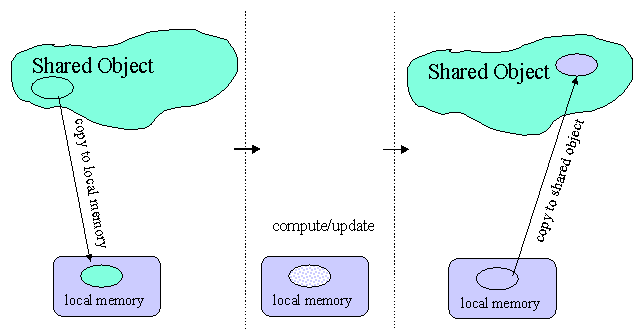
\includegraphics[width=4in]{mod}

The data distribution and locality control are provided to the programmer.  The
data locality information for the shared data is also available.  The library
offers a set of operations for management of its data structures, one-sided
data transfer operations, and supportive operations for data locality control
and queries. The GA shared memory consistency model is a result of a compromise
between the ease of use and a portable performance. The load and store
operations are guaranteed to be \emph{ordered} with respect to each other only
if they target overlapping memory locations. The store operations (\emph{put,
scatter}) and \emph{accumulate} complete locally before returning i.e., the
data in the user local buffer has been copied out but not necessarily completed
at the remote side. The memory consistency is only guaranteed for: 
\begin{itemize}
\item multiple read operations (as the data does not change), 
\item multiple accumulate operations (as addition is commutative), and 
\item multiple disjoint put operations (as there is only one writer for each
element). 
\end{itemize}
The application can manage consistency of its data structures in other cases by
using \emph{lock, barrier}, and \emph{fence} operations available in the
library. 

The data-parallel model is supported by a set of collective functions that
operate on global arrays or their portions. Underneath, if any interprocessor
communication is required, the library uses remote memory copy (most often) or
collective message-passing operations. 

\section{Application Guidelines}

These are some guidelines regarding suitability of the GA for different types
of applications. 

\subsection{When to use GA: }

Algorithmic Considerations 
\begin{itemize}
\item applications with dynamic and irregular communication patterns 
\item for calculations driven by dynamic load balancing 
\item need 1-sided access to shared data structures 
\item need high-level operations on distributed arrays and/or for out-of-core
array-based algorithms (GA + DRA) 
\end{itemize}
Useability Considerations
\begin{itemize}
\item data locality must be explicitly available 
\item when coding in message passing becomes too complicated 
\item when portable performance is important 
\item need object orientation without the overhead of C++ 
\end{itemize}

\subsection{When not to use GA}

Algorithmic Considerations 
\begin{itemize}
\item for systolic, or nearest neighbor communications with regular
communication patterns 
\item when synchronization associated with cooperative point-to-point message
passing is needed (e.g., Cholesky factorization in Scalapack) 
\end{itemize}
Usability Considerations 
\begin{itemize}
\item when interprocedural analysis and compiler parallelization is more
effective 
\item a parallel language support is sufficient and robust compilers available 
\end{itemize}


\chapter{Writing, Building and Running GA Programs}

\chapter{Writing, Building and Running GA Programs}

The GA build process has been improved by using the GNU autotools (autoconf,
automake, and libtool) as well as by combining all of the historic GA libraries
(\texttt{blacklinalg, armci, ma, pario}) into a single, monolithic
\texttt{libga}.  Details on configuring GA can be found by running
``\texttt{configure -{}-help}''. The following sections explain some of the
configure options a typical installation might require for configuring and
building \texttt{libga}, its test programs, and how packages can link to and
use GA. 

The web page \url{www.emsl.pnl.gov/docs/global/support.html} contains
information about using GA on different platforms. Please refer to this page
frequently for most recent updates and platform information.  Information on
building GA on older systems is available in Appendix C, Global Arrays on Older
Systems \ref{Appendix_C}.

\section{Platform and Library Dependencies}

The following platforms are supported by Global Arrays. 

\subsection{Supported Platforms}
\begin{itemize}
\item BlueGene/L 
\item BlueGene/P 
\item Cray XT 
\item Cray XE 
\item Fujitsu 
\item IBM SP
\item Linux Cluster with Ethernet, Myrinet, Infiniband, or Quadrics
\item MAC
\item NEC 
\item SGI Altix
\item Solaris
\item Windows (Cygwin) 
\end{itemize}

For most of the platforms, there are two versions available: 32-bit and 64-bit.
64-bit is preferred and will automatically be selected by the configure script
if the size of the C datatype \texttt{void{*}} is 8 bytes. 

To aid the development of fully portable applications, in 64-bit mode the
Fortran integer datatype is 64-bits. It is motivated by 1) the need of
applications to use very large data structures, and 2) Fortran INTEGER{*}8 not
being fully portable. The 64-bit representation of integer datatype is
accomplished by using the appropriate Fortran compiler flag. The configure
script will determine this flag as needed, but one can always override the
configure script by supplying the environment variable \texttt{FFLAG\_INT} e.g.
\texttt{FFLAG\_INT=-i8}. 

\textbf{Note}: configure almost always does the right thing, so overriding this
particular option is rarely needed. The best way to enforce the integer size of
your choosing is to use the configure options \texttt{-{}-enable-i4} or
\texttt{-{}-enable-i8}. These options will force the integer size to be 4 or 8
bytes in size, respectively. 

Because of limited interest in heterogeneous computing among known us GA users,
the Global Arrays library still does not support heterogeneous platforms. This
capability can be added if required by new applications. 

\subsection{Selection of the communication network for ARMCI}

Some cluster installations can be equipped with a high performance network
which offer instead, or in addition to, TCP/IP some special communication
protocol, for example GM on Myrinet network. To achieve high performance in
Global Arrays, \href{http://www.emsl.pnl.gov/docs/parsoft/armci}{ARMCI} must be
built to use these protocols in its implementation of one-sided communication.
Starting with GA 5.0, this is accomplished by passing an option to the
configure script. 

In addition, it might be necessary to provide a location for the header files
and library path corresponding to the location of software supporting the
appropriate protocol API. 

Our ability to automatically locate the required headers and libraries is
currently inadequate. Therefore, you will likely need to specify the optional
ARG pointing to the necessary directories and/or libraries.  Sockets is the
default ARMCI network if nothing else is specified to configure. Note that the
optional argument ARG takes a quoted string of any CPPFLAGS, LDFLAGS, or LIBS
necessary for locating the headers and libraries of the given ARMCI network. On
many systems it is simply necessary to specify the selected network: 
\begin{verbatim}
./configure --with-openib 
\end{verbatim}
On others, you may need to specify the path to the network's installation if it
is in a non-default location. The following will add
-I/path/to/portals/install/include and -L/path/to/portals/install/lib to the
CPPFLAGS and LDFLAGS if those directories are found to exist: 
\begin{verbatim}
./configure --with-portals="/path/to/portals/install"
\end{verbatim}
See section 2.3.1 for details of what you can pass as the quoted string to
configure options. 

\begin{tabular}{|c|c|>{\centering}p{3cm}|}
\hline 
Network & Protocol Name & Configure Option\tabularnewline
\hline
\hline 
IBM BG/L & BGML & -{}-with-bgml\tabularnewline
\hline 
Cray shmem & Cray shmem & -{}-with-cray-shmem\tabularnewline
\hline 
IBM BG/P & Deep Computing Message Framework & -{}-with-dcmf\tabularnewline
\hline 
IBM LAPI & LAPI & -{}-with-lapi\tabularnewline
\hline 
N/A & MPI Spawn - MPI-2 dynamic process management & -{}-with-mpi-spawn\tabularnewline
\hline 
Infiniband & OpenIB & -{}-with-openib\tabularnewline
\hline 
Cray XT & Portals & -{}-with-portals\tabularnewline
\hline 
Ethernet & TCP/IP & -{}-with-sockets (the default, so you don't need to specify this)\tabularnewline
\hline
\end{tabular}

\subsection{Selection of the message-passing library}
\label{sec:selection-of-the-message-passing-library}

As explained in Section \ref{sec:Initialization-and-Termination}, GA works with
either MPI or TCGMSG message-passing libraries. That means GA applications can
use either of these interfaces. Selection of the message-passing library takes
place when GA is configured.  Since the TCGMSG library is small and compiles
fast, it is included with the GA distribution package but as of GA 5.0 it is no
longer built by default. For GA 5.0, MPI is the default message-passing
library.  There are three possible configurations for running GA with the
message-passing libraries:

\begin{enumerate}

\item \underbar{GA with MPI} (\emph{recommended}): directly with MPI. In this
mode, GA program should contain MPI initialization calls. Example:
\texttt{./conifigure}

\item \underbar{GA with TCGMSG-MPI} (MPI and TCGMSG emulation library):
TCGMSG-MPI implements functionality of TCGMSG using MPI.  In this mode, the
message passing library can be initialized using either TCGMSG PBEGIN(F) or
MPI\_Init. Example: \texttt{./configure -{}-with-mpi -{}-with-tcgmsg}

\item \underbar{GA with TCGMSG}: directly with TCGMSG.  In this mode, GA
program should contain TCGMSG initialization calls.  Example:\texttt{
./configure -{}-with-tcgmsg}

\end{enumerate}

For the MPI versions (1 and 2 above), the \texttt{-{}-with-mpi} configure
option can take parameters. If no parameters are specified, configure will
search for the MPI compilers. Using the MPI compilers is the recommended way to
build GA. If the MPI compilers are not found, configure will exit with an
error. The configure script will attempt to determine the underlying Fortran
77, C, and C++ compilers wrapped by the MPI compilers. This is necessary for
other configure tests such as determining compiler-specific optimization flags
or determining the Fortran 77 libraries needed when linking using the C++
linker.

If an argument is specified to \texttt{-{}-with-mpi}, then configure will no
longer use the MPI compilers. Instead, configure will attempt to located the
MPI headers and libraries. The locations of the headers and the locations and
names of the one or more MPI libraries can differ wildly. The argument to
\texttt{-{}-with-mpi} can be a quoted string of any install paths, include
paths, library paths, and/or libraries required for compiling and linking MPI
programs. See section 2.3.1 for details of the possible arguments. 

\subsection{Dependencies on other software}

In addition to the message-passing library, GA requires (internally):

\begin{itemize}

\item \href{http://www.emsl.pnl.gov/docs/parsoft/ma/MAapi.html}{MA} (Memory
Allocator), a library for managment of local memory; 

\item \href{http://www.emsl.pnl.gov/docs/parsoft/armci}{ARMCI}, a one-sided
communication library that GA uses as its run-time system; 

\end{itemize}

GA optionally can use external: 

\begin{itemize}

\item BLAS library is required for the eigensolver and \texttt{ga\_dgemm}
(a subset is included with GA, which is built into \texttt{libga.a});

\item LAPACK library is required for the eigensolver (a subset is included
with GA, which is built into \texttt{libga.a}); 

\end{itemize}

GA may also depend on other software depending on the functions being
used.

\begin{itemize}

\item GA eigensolver, ga\_diag, is a wrapper for the eigensolver from the
PEIGS library; (Please contact \href{mailto:fanngi@ornl.gov}{George Fann}about
PEIGS) 

\item SCALAPACK, PBBLAS, and BLACS libraries are required for \emph{ga\_lu\_solve,
ga\_cholesky, ga\_llt\_solve, ga\_spd\_invert, ga\_solve}. If these
libraries are not installed, the named operations will not be available. 

\end{itemize}

\section{Writing GA Programs}

C programs that use Global Arrays should include files \emph{'ga.h'} and
\emph{`macdecls.h'}. Fortran programs should include the files
\emph{`mafdecls.fh'} and \emph{`global.fh'}. Fortran source must be
preprocessed as a part of compilation.

The GA program should look like:
\begin{itemize}
\item When GA runs with MPI
\end{itemize}
\input{mpif.tex}
\input{mpic.tex}
\begin{itemize}
\item When GA runs with TCGMSG or TCGMSG-MPI
\end{itemize}
\input{tcgmsgf.tex}
\input{tcgmsgc.tex}
{*}{*}The \emph{ma\_init} call looks like:
\begin{verbatim}
status = ma_init(type, stack_size, heap_size)
\end{verbatim}
and it basically just goes to the OS and gets \emph{stack\_size+heap\_size}
elements of size \emph{type}. The amount of memory MA allocates need to be
sufficient for storing global arrays on some platforms. Please refer to section
\ref{sub:Memory-Allocation} for the details and information on more advanced
usage of MA in GA programs. 

\section{Building GA}

GNU Autotools (autoconf, automake, and libtool) are used to help build the GA
library and example programs. GA follows the usual convention of:
\begin{verbatim}
./configure; make; make install 
\end{verbatim}
Before GA 5.0 the user was required to set a TARGET environment variable. This
is no longer required - the configure script will determine the TARGET for the
user. The configure script will also search for appropriate Fortran 77, C, and
C++ compilers. To override the compilers, set the F77, CC, and/or CXX
environment variables or specify them to configure:
\begin{verbatim}
./configure CC=gcc F77=ifort CFLAGS="-O2 -g -Wall"
\end{verbatim}
For the complete list of environment variables which configure recognizes, see
the output of running: 
\begin{verbatim}
./configure --help
\end{verbatim}

\subsection{Building and Running GA Test and Example Programs}

The GA distribution comes with a number of test and example programs located in
./global/testing and ./global/examples, respectively. To build these programs,
after running configure and make, run the additional make target: 
\begin{verbatim}
make checkprogs
\end{verbatim}
To run the GA test suite, you must tell the make program how to run parallel
programs. The following assumes either an interactive session on a queued
system or a workstation: 
\begin{verbatim}
make check MPIEXEC="mpirun -np 4"
\end{verbatim}
Of course, replace the value of MPIEXEC to the appropriate command for the MPI
implementation used to build GA. The test suite has not been tested with the
TCGMSG message-passing library's parallel.x invoker. 

\subsection{Configure Options which Take Arguments}

Certain configure options take arguments which help the configure script locate
the headers and libraries necessary for the particular software. For example,
when specifying the ARMCI network (see section 2.1.2), the location of the MPI
installation (see section 2.1.3), or specifying the location of other external
software such as BLAS, LAPACK, or ScaLAPACK. 

You can put almost anything into the quoted argument to these configure
options. For example,\texttt{ -I{*}, -L{*}, -l{*}, -Wl{*}, -WL{*}, {*}.a,
{*}.so} where the asterisk represents the usual arguments to those compiler and
linker flags or paths to static or shared libraries.  Here are some sample MPI
uses to illustrate our point:
\begin{verbatim}
--with-mpi="/usr/local"
--with-mpi="-I/usr/local/include -L/usr/local/lib -lmpi"
--with-mpi="-lmpichf90 -lmpich"
\end{verbatim}

\subsection{BLAS and LAPACK}

The GA distribution contains a subset of the BLAS and LAPACK routines necessary
for successfully linking GA programs. However, those routines are not
optimized. If optimized BLAS and LAPACK routines are available on your system,
we recommend using them. The configure script will automatically attempt to
locate external BLAS and LAPACK libraries. 

Correctly determining the size of the Fortran INTEGER used when compiling
external BLAS and LAPACK libraries is not automatic. Even on 64-bit platforms,
external BLAS libraries are often compiled using 4-byte Fortran INTEGERs. The
GA interface to the BLAS and LAPACK routines must match the Fortran INTEGER
size used in the external BLAS and LAPACK routines. There are three options to
configure: 
\begin{itemize}
\item \texttt{-{}-with-blas{[}=ARG{]}} is the default and will attempt to
detect the size of the INTEGER, but if it fails (and it often will since this
is no easy task), it will assume 4-byte INTEGERS. Automatic detection of the
INTEGER size may improve in the future.
\item \texttt{-{}-with-blas4{[}=ARG{]}} assumes 4-byte INTEGERs 
\item \texttt{-{}-with-blas8{[}=ARG{]}} assumes 8-byte INTEGERs 
\end{itemize}
If LAPACK is in a separate library, you may need to specify
\texttt{-{}-with-lapack=ARG} where ARG is the path to the LAPACK library. See
section 2.3.1 for details. 

\subsection{ScaLAPACK}

GA interface routines to ScaLAPACK are only available when GA is built with MPI
and ScaLAPACK. Before building GA, the user is required to configure
-{}-with-scalapack and pass the location of ScaLAPACK \& Co. libraries passed
as arguments to those configure options. See section 2.3.2 (Configure Options
which Take Arguments) for details. 

\subsection{GA C++ Bindings}

The configure script automatically determines the Fortran 77 libraries required
for linking a C++ application and places them in the FLIBS variable within the
generated Makefile. Building the C++ bindings is then as simple as specifying: 
\begin{verbatim}
./configure --enable-cxx
\end{verbatim}
Running make will then link the libga++.a library in addition to the libga.a
library. Both are then required for linking C++ GA applications, specifying
libga++.a first and then libga.a (typically as -lga++ -lga). 

\subsection{Disabling Fortran}

Fortran sources have typically been used by the GA and ARMCI distributions.
For GA 5.0 and beyond, Fortran sources have been deprecated in the ARMCI
distribution and are still used by default in the GA source.  Therefore, ARMCI
is free from Fortran dependencies while GA is not.  The GA dependencies can be
removed by specifying 
\begin{verbatim}
./configure --disable-f77
\end{verbatim}
Note that disabling Fortran 77 in GA is not well tested and doing so will also
likely disable the use of external Fortran 77 libraries such as Fortran-based
BLAS or ScaLAPACK. This also disables the use of the GA library in Fortran
applications since the MA sources will no longer be compiled with Fortran 77
support. Use this option with care and only if developing C and/or C++
applications exclusively. 

\subsection{Python Bindings}

GA 5.0 releases with Python bindings which were developed using the Cython
package (http://www.cython.org/). At a minimum, GA must be configured with
shared library support (which is disabled by default.) The configure script
will automatically search for a python interpreter in the PATH environment
variable, so make sure the appropriate Python interpreter can be found before
configuring. For example: 
\begin{verbatim}
./configure --enable-shared
\end{verbatim}
should be all that is required to enable Python bindings. The Python bindings
are not installed by default. You should run the following: 
\begin{verbatim}
make python
\end{verbatim}
in order to build and install the Python bindings. The python make target
depends on the install target (i.e. ``make install'') and will pass the
libga.so and ga.h library and header locations to the python setup.py
invocation. Optionally, you can navigate to the python source directory and
run: 
\begin{verbatim}
python setup.py build_ext
\end{verbatim}
or 
\begin{verbatim}
python setup.py build_ext --inplace
\end{verbatim}
to build the python bindings in a more manual way. The ``make python'' target
is not well tested since specifying dependent libraries can be a difficult
task. 

If GA was built with external BLAS and LAPACK, those libraries must be
specified when linking the Python shared library. Currently, users must edit
the setup.py script within the python source directory in order to add these
libraries to the standard distutils invocation of the linker. The BLAS and
LAPACK libraries on OSX are particularly difficult to find, so this is done
automatically for the user since the configure script will detect the vecLib
framework on OSX automatically.  Unforunately, at this time bulding the Python
bindings is often a manual process but those fluent in Python and Python's
\texttt{distutils} should have few problems editing the \texttt{setup.py}
script. 

\subsection{Writing and Building New GA Programs}

As of GA 5.0, the ability to place small single-file test programs into the
global/testing directory of the distribution is no longer supported. Instead,
you must install the GA headers and libraries using the ``make install''
target.

This will install the GA headers and libraries to the location specified by the
-{}-prefix configure option. If not specified, the default is
\texttt{/usr/local/include} and \texttt{/usr/local/lib}.  For our testing
purposes, we often install GA into the same location as the build. Recall, GA
can be configured from a separate build directory, keeping source and build
trees separate. For example, from the top-level GA source distribution: 
\begin{verbatim}
mkdir bld
cd bld
../configure --prefix=`pwd`
make
make install
\end{verbatim}
will configure, build, and install the GA headers and library into the separate
build directory ``bld''.

More specifically, you would find the GA library \texttt{libga} in
\texttt{./bld/lib} and the GA headers in \texttt{./bld/include}. For packages
using GA, you need to provide appropriate compiler and linker flags to indicate
the locations of the GA header files and libraries. 

\section{Running GA Programs}

Assume the GA program app.x had already been built. To run it,

\emph{Running on shared memory systems and clusters}: (i.e., network of
workstations/linux clusters)

If the app.x is built based on MPI, run the program the same way as any other
MPI programs. 

\emph{Example}: to run on four processes on clusters, use 
\begin{verbatim}
mpirun -np 4 app.x
\end{verbatim}
\emph{Example}: If you are using MPICH (or MPICH-like Implementations), and
mpirun requires a machinefile or hostfile, then run the GA program same as any
other MPI programs. \textit{The only change required is to make sure the
hostnames are specified in a consecutive manner in the machinefile}. Not doing
this will prevent SMP optimizations and would lead to poor resource
utilization.
\begin{verbatim}
mpirun -np 4 -machinefile machines.txt app.x
\end{verbatim}
\emph{Contents of machines.txt}: Let us say we have two 2-way SMP
nodes (host1 and host2, and correct formats for a 4-processor machinefile
is shown in the table below.

\begin{tabular}{|>{\centering}p{2cm}|>{\centering}p{2cm}|>{\raggedright}p{3cm}|}
\hline 
Correct & Correct & Incorrect\tabularnewline
\hline
\hline 
host1

host1

host2

host2 & host2

host2

host1

host1 & host1

host2

host1 (This is wrong, the same hosts should be specified together)

host2\tabularnewline
\hline
\end{tabular}

If app.x is built based on TCGMSG (not including Fujitsu, Cray J90, and
Windows, because there are no native ports of TCGMSG), to execute the program
on Unix workstations/servers, one should use the 'parallel.x' program. After
building the application, a file called 'app.x.p' would also be generated (If
there is not such a file, make it: 
\begin{verbatim}
make app.x.p
\end{verbatim}
This file can be edited to specify how many processors and tasks to use, and
how to load the executables. Make sure that 'parallel.x' is accessible (you
might copy it into your 'bin' directory). To execute, type:
\begin{verbatim}
parallel.x app.x
\end{verbatim}

\begin{enumerate}

\item On MPPs, such as Cray XT3/XT4, or IMB SPs, use the appropriate system
command to specify the number of processors, load and run the programs.
Example: 
\begin{itemize}
\item to run on IBM SP, run as any other parallel programs (i.e., using
\emph{poe}) 
\item to run on Cray XT3/XT4, use \emph{yod}.
\end{itemize}

\item On Microsoft NT, there is no support for TCGMSG, which means you can only
build your application based on MPI. Run the application program the same way
as any other MPI programs. For, WMPI you need to create the .pg file. Example:
\begin{verbatim}
R:\nt\g\global\testing> start /b test.x.exe
\end{verbatim}
\end{enumerate}

\section{Building Intel Trace Analyzer (VAMPIR) Instrumented Global Arrays}

Building GA for use with the intel trace analyzer is no loger supported. As of
GA 5.1 allows the GA functions to be intercepted by user code.

TODO TODO TODO describe new pnga\_ interfaces


\chapter{\label{sec:Initialization-and-Termination}Initialization and Termination}

\chapter{Initialization and Termination}
\label{sec:Initialization-and-Termination}

For historical reasons (the 2-dimensional interface was developed first), many
operations have two interfaces, one for two dimensional arrays and the other
for arbitrary dimensional (one- to seven- dimensional, to be more accurate)
arrays. The latter can definitely handle two dimensional arrays as well. The
supported data types are integer,double precision, and double complex. Global
Arrays provide C and Fortran interfaces in the same (mixed-language) program to
the same array objects. The underlying data layout is based on the Fortran
convention.

GA programs require message-passing and Memory Allocator (MA) libraries to
work. Global Arrays is an extension to the message-passing interface.  GA
internally does not allocate local memory from the operating system - all
dynamically allocated local memory comes from MA. We will describe the details
of memory allocation later in this section. 

\section{Message Passing}

The first version of Global Arrays was released in 1994 before robust MPI
implementations became available. At that time, GA worked only with TCGMSG, a
message-passing library that one of the GA authors (Robert Harrison) had
developed before. In 1995, support for MPI was added. At the present time, the
GA distribution still includes the TCGMSG library for backward compatibility
purposes, and because it is small, fast to comple, and provides a minimal
message-passing support required by GA programs. The MPI-compatible version of
GA became the default as of version 5.0. See
\ref{sec:selection-of-the-message-passing-library} for details.

The GA toolkit needs the following functionality from any message-passing
library it runs with:
\begin{itemize}
\item initialization and termination of processes in an SPMD
(single-program-multiple-data) program, 
\item synchronization, 
\item functions that return number of processes and calling process id, 
\item broadcast, 
\item reduction operation for integer and double datatypes, and 
\item a function to abort the running parallel job in case of an error.
\end{itemize}
The message-passing library has to be initialized before the GA library and
terminated after the GA library is terminated.

GA provides two functions \emph{ga\_nnodes} and \emph{ga\_nodeid} that return
the number of processes and the calling process id in a parallel program.
Starting with release 3.0, these functions return the same values as their
message-passing counterparts. In earlier releases of GA on clusters of
workstations, the mapping between GA and message-passing process ids were
nontrivial. In these cases, the \emph{ga\_list\_nodeid} function (now obsolete)
was used to describe the actual mapping.

Although message-passing libraries offer their own barrier (global
synchronization) function, this operation does not wait for completion of the
outstanding GA communication operations. The GA toolkit offers a
\emph{ga\_sync} operation that can be used for synchronization, and it has the
desired effect of waiting for all the outstanding GA operations to complete. 

\section{Memory Allocation}
\label{sub:Memory-Allocation}

GA uses a very limited amount of statically allocated memory to maintain its
data structures and state. Most of the memory is allocated dynamically as
needed, primarily to store data in newly allocated global arrays or as
temporary buffers internally used in some operations, and deallocated when the
operation completes.

There are two flavors of dynamically allocated memory in GA: shared memory and
local memory. Shared memory is a special type of memory allocated from the
operating system (UNIX and Windows) that can be shared between different user
processes (MPI tasks). A process that attaches to a shared memory segment can
access it as if it was local memory. All the data in shared memory is directly
visible to every process that attaches to that segment. On shared memory
systems and clusters of SMP (symmetritc multiprocessor) nodes, shared memory is
used to store global array data and is allocated by the Global Arrays run-time
system called ARMCI. ARMCI uses shared memory to optimize performance and avoid
explicit interprocessor communication within a single shared memory system or
an SMP node. ARMCI allocates shared memory from the operating system in large
segments and then manages memory in each segment in response to the GA
allocation and deallocation calls. Each segment can hold data in many small
global arrays. ARMCI does not return shared memory segments to the operating
system until the program terminates (calls \emph{ga\_terminate}).

On systems that do not offer shared-memory capabilities or when a program is
executed in a serial mode, GA uses local memory to store data in global arrays.

All of the dynamically allocated local memory in GA comes from its companion
library, the Memory Allocator (MA) library. MA allocates and manages local
memory using stack and heap disciplines. Any buffer allocated and deallocated
by a GA operation that needs temporary buffer space comes from the MA stack.
Memory to store data in global arrays comes from heap. MA has additional
features useful for program debugging such as:
\begin{itemize}
\item left and right guards: they are stamps that detect if a memory segment
was overwritten by the application, 
\item named memory segments, and 
\item memory usage statistics for the entire program.
\end{itemize}
Explicit use of MA by the application to manage its non-GA local data
structures is not necessary but encouraged. Because MA is used implicitly by
GA, it has to be initialized before the first global array is allocated.  The
\emph{MA\_init} function requires users to specify memory for heap and stack.
This is because MA:
\begin{itemize}
\item allocates from the operating system only one segment equal in size to the
sum of heap and stack, 
\item manages both allocation schemes using memory coming from opposite ends of
the same segment, and 
\item the boundary between free stack and heap memory is dynamic.
\end{itemize}
It is not important what the stack and heap size argument values are
as long as the aggregate memory consumption by a program does not
exceed their sum at any given time. 

MA is optional for C programs. You can replace GA's internal MA memory handling
with \texttt{malloc()} and \texttt{free()} by using the function
\texttt{GA\_Register\_stack\_memory()}.
\input{replace_ma.tex}

\subsection{Determining the Values of MA Stack and Heap Size}

How can I determine what the values of MA stack and heap size should be? 

The answer to this question depends on the run-time environment of the program
including the availability of shared memory. A part of GA initialization
involves initialization of the ARMCI run-time library.  ARMCI dynamically
determines if the program can use shared memory based on the architecture type
and current configuration of the SMP cluster. For example, on uniprocessor
nodes of the IBM SP shared memory is not used whereas on the SP with SMP nodes
it is. This decision is made at run-time. GA reports the information about the
type of memory used with the function \emph{ga\_uses\_ma()}. This function
returns false when shared memory is used and true when MA is used.

Based on this information, a programmer who cares about the efficient usage of
memory has to consider the amount of memory per single process (MPI task)
needed to store data in global arrays to set the heap size argument value in
ma\_init. The amount of stack space depends on the GA operations used by the
program (for example \emph{ga\_mulmat\_patch} or \emph{ga\_dgemm} need several
MB of buffer space to deliver good performance) but it probably should not be
less than 4MB.  The stack space is only used when a GA operaion is executing
and it is returned to MA when it completes. 

\section{GA Initialization}

The GA library is initialized after a message-passing library and before MA. It
is possible to initialize GA after MA but it is not recommended: GA must first
be initialized to determine if it needs shared or MA memory for storing
distributed array data. There are two alternative functions to initialize GA:

TODO
%\begin{verbatim}
%Fortran  subroutine GA_initialize()
%C        void GA_Initialize()
%C++      void GA::Initialize(int argc, char **argv)
%\end{verbatim}

and

TODO
%\begin{verbatim}
%Fortran  subroutine GA_Initialize_ltd(limit)
%C        void GA_Initialize_ltd(size_t limit) 
%C++      void GA::Initialize(int argc, char **argv, size_t limit)
%\end{verbatim}

The first interface allows GA to consume as much memory as the application
needs to allocate new arrays. The latter call allows the programmer to
establish and enforce a limit within GA on the memory usage.

\emph{Note}: In GA++, there is an additional functionality as follows: 

TODO 
%\begin{verbatim}
%C++      void GA::Initialize(int argc, char *argv[], 
%         unsigned long heapSize, unsigned long stackSize,
%         int type, size_t limit=0) 
%\end{verbatim}

\subsection{Limiting Memory Usage by Global Arrays}

GA offers an optional mechanism that allows a programmer to limit the aggregate
memory consumption used by GA for storing Global Array data. These limits apply
regardless of the type of memory used for storing global array data.They do not
apply to temporary buffer space GA might need to use to execute any particular
operation. The limits are given per process (MPI task) in bytes. If the limit
is set, GA would not allocate more memory in global arrays that would exceed
the specified value - any calls to allocate new arrays that would simply fail
(return false). There are two ways to set the limit:
\begin{enumerate}
\item at initialization time by calling ga\_initialize\_ltd, or 
\item after initialization by calling the function
\end{enumerate}

TODO
%\begin{verbatim}
%Fortran  subroutine ga_set_memory_limit(limit) 
%C        void GA_Set_memory_limit(size_t limit) 
%C++      void GA::GAServices::setMemoryLimit(size_t limit)
%\end{verbatim}

It is encouraged that the user choose the first option, even though the user
can intialize the GA normally and set the memory limit later.

\emph{Example}: Initialization of MA and setting GA memory limits
\begin{verbatim}
call ga_initialize() 
if (ga_uses_ma()) then
   status = ma_init(MT_DBL, stack, heap+global) 
else 
   status = ma_init(mt_dbl,stack,heap) 
call ga_set_memory_limit(ma_sizeof(MT_DBL,global,MT_BYTE)) 
endif 
if(.not. status) ... !we got an error condition here
\end{verbatim}
In this example, depending on the value returned from ga\_uses\_ma(), we either
increase the heap size argument by the amount of memory for global arrays or
set the limit explicitly through ga\_set\_memory\_limit().  When GA memory
comes from MA we do not need to set this limit through the GA interface since
MA enforces its memory limits anyway. In both cases, the maximum amount of
memory acquired from the operating system is capped by the value
\emph{stack+heap+global}. 

\section{Termination}

The normal way to terminate a GA program is to call the function

TODO
%\begin{verbatim}
%Fortran  subroutine ga_terminate() 
%C        void {GA_Terminate() 
%C++      void GA::Terminate()
%\end{verbatim}

The programmer can also abort a running program for example as part
of handling a programmatically detected error condition by calling
the function

TODO
%\begin{verbatim}
%Fortran  subroutine ga_error(message, code)
%C        void GA_Error(char *message, int code)
%C++      void GA::GAServices::error(char *message, int code)
%\end{verbatim}

\section{Creating Arrays - I}

There are three ways to create new arrays:
\begin{enumerate}
\item From scratch, for regular distribution, using

TODO
%\begin{verbatim}
%n-d Fortran  logical function nga_create(type, ndim, 
%                        dims, array_name, chunk, g_a) 
%2-d Fortran  logical function ga_create(type, dim1, 
%
%                        dim2, array\_name, chunk1, chunk2, g\_a) 
%
%{C}           int {NGA\_{}Create}(int type, int ndim, int dims{[}{]}, 
%
%                        char {*}array\_name, int chunk{[}{]}) 
%
%{C++}         GA::GlobalArray{*} GA::GAServices::createGA(int type, 
%
%                        int ndim, int dims{[}{]}, char {*}array\_name, 
%
%                        int chunk{[}{]})
%\end{verbatim}

or for regular distribution, using

TODO
%\begin{verbatim}
%{n-d} {Fortran} logical function {nga\_{}create\_{}irreg}(type, ndim, dims,
%
%                       array\_name, map, nblock, g\_a) 
%
%{2-d} {Fortran} logical function {ga\_{}create\_{}irreg}(type, dim1, dim2,
%
%                       array\_name, map1, nblock1, map2, nblock2, g\_a) 
%
%C           int {NGA\_{}Create\_{}irreg}(int type, int ndim, int dims{[}{]}, 
%
%C++         GA::GlobalArray{*} GA::GAServices::createGA(int type, 
%
%                       int ndim, int dims{[}{]}, char {*}array\_name, 
%
%                       int map{[}{]}, int block{[}{]})
%\end{verbatim}

\item Based on a template (an existing array) with the function

TODO
%\begin{verbatim}
%{Fortran} logical function {ga\_{}duplicate}(g\_a, g\_b, array\_name) 
%
%{C}       int {GA\_{}Duplicate}(int g\_a, char {*}array\_name) 
%
%{C++}     int {GA::GAServices::duplicate}(int g\_a, char {*}array\_name) 
%
%- or - 
%
%{C++}     GA::GlobalArray{*} GA::GAServices::createGA(int g\_a, char
%
%                         {*}array\_name)
%\end{verbatim}

\item Refer to the ``Creating Arrays - II'' section.
\end{enumerate}

In this case, the new array inherits all the properties such as distribution,
datatype and dimensions from the existing array.

With the regular distribution shown in Figure \ref{cap:RegularDistribution},
the programmer can specify block size for none or any dimension. If block size
is not specified the library will create a distribution that attempts to assign
the same number of elements to each processor (for static load balancing
purposes). The actual algorithm used is based on heuristics.

\begin{figure}
\begin{centering}
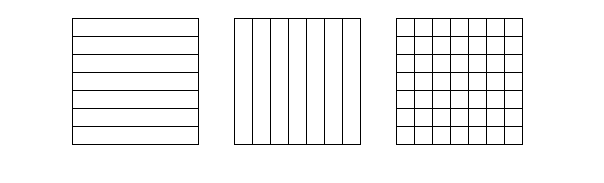
\includegraphics[width=0.9\columnwidth]{distr-1}
\caption{Regular Distribution}
\label{cap:RegularDistribution}
\end{centering}
\end{figure}

With the irregular distribution shown in Figure
\ref{cap:IrregularDistribution}, the programmer specifies distribution points
for every dimension using map array argument. The library creates an array with
the overall distribution that is a Cartesian product of distributions for each
dimension. A specific example is given in the documentation.

\begin{figure}
\begin{centering}
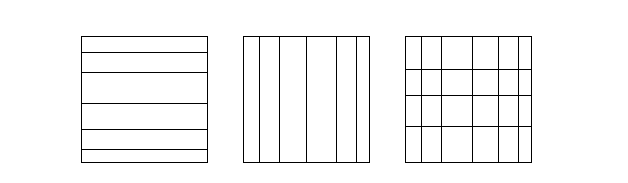
\includegraphics[width=0.9\columnwidth]{distr-2}
\caption{Irregular Distribution}
\label{cap:IrregularDistribution}
\end{centering}
\end{figure}

If an array cannot be created, for example due to memory shortages or an
enforced memory consumption limit, these calls return failure status. Otherwise
an integer handle is returned. This handle represents a global array object in
all operations involving that array. This is the only piece of information the
programmer needs to store for that array. All the properties of the object
(data type, distribution data, name, number of dimensions and values for each
dimension) can be obtained from the library based on the handle at any time,
see Section 7.4. It is not necessary to keep track of this information
explicitly in the application code.

Note that regardless of the distribution type at most one block can be
owned/assigned to a processor. 

\subsection{Creating Arrays with Ghost Cells}

Individual processors ordinarily only hold the portion of global array data
that is represent by the lo and hi index arrays returned by a call to
nga\_distribution or that have been set using the nga\_create\_irreg call.
However, it is possible to create global arrays where this data is padded by a
boundary region of array elements representing portions of the global array
residing on other processors. These boundary regions can be updated with data
from neighboring processors by a call to a single GA function. To create global
arrays with these extra data elements, referred to in the following as ghost
cells, the user needs to call either the functions:

TODO
%\begin{verbatim}
%{n-d} Fortran logical function {nga\_{}create\_{}ghosts}(type, dims, width,
%
%                            array\_name, chunk, g\_a)
%
%{C}           int int {NGA\_{}Create\_{}ghosts}(int type, int ndim, int dims{[}{]},
%
%                            int width{[}{]}, char {*}array\_name, int chunk{[}{]})
%
%{C++}         int GA::GAServices::createGA\_GhostsGA\_Ghosts(int type, int
%
%                            ndim, int dims{[}{]},int width{[}{]}, 
%
%                            char  {*}array\_name, int chunk{[}{]})
%
%{n-d Fortran} logical function {nga\_{}create\_{}ghosts\_{}irreg}(type, dims, width,
%
%                            array\_name, map, block, g\_a) 
%
%{C}           int int {NGA\_{}Create\_{}ghosts\_{}irreg}(int type, int ndim, 
%
%                            int dims{[}{]}, int width{[}{]}, char {*}array\_name,
%
%                            int map{[}{]}, int block{[}{]}) 
%
%{C++}         int GA::GAServices::createGA\_Ghosts(int type, int ndim, 
%
%                            int dims{[}{]}, int width{[}{]}, char {*}array\_name,
%
%                            int map{[}{]}, int block{[}{]}) 
%
%
%\end{verbatim}

These two functions are almost identical to the \texttt{nga\_create} and
\texttt{nga\_create\_irreg} functions described above. The only difference is
the parameter array width. This is used to control the width of the ghost cell
boundaries in each dimension of the global array. Different dimensions can be
padded with different numbers of ghost cells, although it is expected that for
most applications the widths will be the same for all dimensions. If the width
has been set to zero for all dimensions, then these two functions are
completely equivalent to the functions \texttt{nga\_create} and
\texttt{nga\_create\_irreg}. 

To illustrate the use of these functions, an ordinary global array is shown in
Figure \ref{cap:OrdinaryGlobalArray}. The boundaries represent the data that is
held on each processor.

\begin{figure}
\begin{centering}
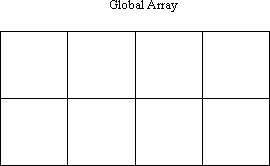
\includegraphics[width=0.9\columnwidth]{ghost003}
\caption{Ordinary Global Array}
\label{cap:OrdinaryGlobalArray}
\end{centering}
\end{figure}

For a global array with ghost cells, the data distribution can be visualized as
shown in Figure \ref{cap:GAwGhostCells}:

\begin{figure}
\begin{centering}
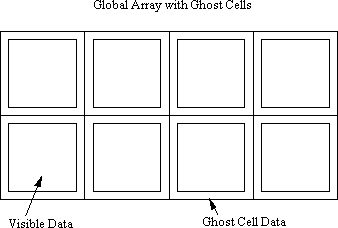
\includegraphics[width=0.9\columnwidth]{ghost006}
\caption{Global Array with Ghost Cells}
\label{cap:GAwGhostCells}
\end{centering}
\end{figure}

Each processor holds ``visible'' data, corresponding to the data held on each
processor of an ordinary global array, and ``ghost cell'' data, corresponding
to neighboring points in the global array that would ordinarily be held on
other processors. This data can be updated in a single call to
\texttt{nga\_update}, described under the collective operations section of the
user documentation. Note that the ghost cell data duplicates some portion of
the data in the visible portion of the global array. The advantage of having
the ghost cells is that this data ordinarily resides on other processors and
can only be retrieved using additional calls. To access the data in the ghost
cells, the user must use the \texttt{nga\_access\_ghosts} function described in
Section 6.1. 

\section{Creating Arrays - II}

As mentioned in the previous section (``Creating arrays - I''), there are 3
ways to create arrays. This section describes method \#3 to create arrays.
Because of the increasingly varied ways that global arrays can be configured, a
set of new interfaces for creating global arrays has been created. This
interface supports all the configurations that were accessible via the old
ga\_create\_XXX calls, as well as new options that can only be accessed using
the new interface. Creating global arrays using the new interface starts by a
call to ga\_create\_handle that returns the user a new global array handle. The
user then calls several ga\_set\_XXX calls to assign properties to this handle.
These properties include the dimension of the array, the data type, the size of
the array, and any other properties that may be relevant. At present, the
available ga\_set\_XXX calls largely reflect properties that are accessible via
the nga\_create\_XXX calls, however, it is anticipated that the range of
properties that can be set using these calls will expand considerably in the
future.  After all the properties have been set, the user calls ga\_allocate on
the array handle and memory is allocated for the array. The array can now be
used in exactly the same way as arrays created using the traditional
ga\_create\_XXX calls. The calls for obtaining a new global array handle are

TODO
%\begin{verbatim}
%{n-d Fortran} integer function {ga\_{}create\_{}handle}() 
%
%{C}           int {GA\_{}Create\_{}handle}()
%\end{verbatim}

Properties of the global arrays can be set using the ga\_set\_XXX
calls. Note that the only required call is to ga\_set\_data. The others
are all optional.

TODO
%\begin{verbatim}
%{n-d Fortran} subroutine {ga\_{}set\_{}data}(g\_a, ndim, dims, type) 
%
%{C}           void {GA\_{}Set\_{}data}(int g\_a, int ndim, int {*}dims, int type)
%\end{verbatim}

The argument \emph{g\_a} is the global array handle, \emph{ndim} is the
dimension of the array, \emph{dims} is an array of \emph{ndim} numbers
containing the dimensions of the array, and \emph{type} is the data type as
defined in either the macdecls.h or mafdecls.h files.  Other options that can
be set using these subroutines are:

TODO
%\begin{verbatim}
%{n-d Fortran} subroutine {ga\_{}set\_{}array\_{}name}(g\_a, array\_name) 
%
%{C}           void {GA\_{}Set\_{}array\_{}name}(int g\_a, char {*}array\_name)
%\end{verbatim}

This subroutine assigns a character string as an array name to the
global array.

TODO
%\begin{verbatim}
%{n-d Fortran} subroutine {ga\_{}set\_{}chunk}(g\_a, chunk) 
%
%C           void {GA\_{}Set\_{}chunk}(int g\_a, int {*}chunk)
%\end{verbatim}

The chunk array contains the minimum size dimensions that should be allocated
to a single processor. If the minimum size is set to -1 for some of the
dimensions, then the minimum size allocation is left to the GA toolkit. The
default setting of the chunk array is -1 along all dimensions.

TODO
%\begin{verbatim}
%{n-d Fortran} subroutine {ga\_{}set\_{}irreg\_{}distr}(g\_a, map, block) 
%
%{C}           void {GA\_{}Set\_{}irreg\_{}distr}(int g\_a, int {*}map, int {*}block)
%\end{verbatim}

The ga\_set\_irreg\_distr subroutine can be used to specify the distribution of
data among processors. The block array contains the processor grid used to lay
out the global array and the map array contains a list of the first indices of
each block along each of the array axes. If the first value in the block array
is M, then the first M values in the map array are the first indices of each
data block along the first axis in the processor grid. Similarly, if the second
value in the block array is N, then the values in the map array from M+1 to M+N
are the first indices of the each data block along the second axis and so on
through the D dimensions of the global array.

TODO
%\begin{verbatim}
%{n-d Fortran} subroutine {ga\_{}set\_{}ghosts}(g\_a, width) 
%
%{C}           void {GA\_{}Set\_{}ghosts}(int g\_a, int {*}width)
%\end{verbatim}

This call can be used to set the ghost cell width along each of the array
dimensions.

TODO
%\begin{verbatim}
%{n-d Fortran} subroutine {ga\_{}set\_{}pgroup}(g\_a, p\_group) 
%
%{C}           void {ga\_{}set\_{}pgroup}(int g\_a, int p\_group)
%\end{verbatim}

This call assigns a processor group to the global array. If no processor group
is assigned to the global array, it is assumed that the global array is created
on the default processor group.

After all the array properties have been set, memory for the global array is
allocated by a call to ga\_allocate. After this call, the global array is ready
for use inside the parallel application.

TODO
%\begin{verbatim}
%{n-d Fortran} logical function {ga\_{}allocate}(g\_a) 
%
%{C}           int {GA\_{}Allocate}(int g\_a)
%\end{verbatim}

This function returns a logical variable that is true if the global array was
successfully allocated and false otherwise. 

\section{Destroying Arrays}

Global arrays can be destroyed by calling the function

TODO
%\begin{verbatim}
%{Fortran} logical {ga\_{}destroy}(g\_a) 
%
%{C}       void {GA\_{}Destroy}(int g\_a) 
%
%{C++}     void GA::GlobalArray::destroy()
%\end{verbatim}

that takes as its argument a handle representing a valid global array.  It is a
fatal error to call ga\_destroy with a handle pointing to an invalid array.

All active global arrays are destroyed implicitly when the user calls
\texttt{ga\_terminate}.


\chapter{One-sided Communication Operations}

\chapter{One-sided Communication Operations}

Global Arrays provide one-sided, noncollective communication operations
that allow to access data in global arrays without cooperation with
the process or processes that hold the referenced data. These processes
do not know what data items in their own memory are being accessed
or updated by remote processes. Moreover, since the GA interface uses
global array indices to reference nonlocal data, the calling process
does not even have to know process ids and location in memory where
the refernenced data resides.

The one-sided operations that Global Arrays provide can be summarized
into three categories: 

\begin{tabular}{|>{\centering}p{4cm}|>{\centering}p{4cm}|}
\hline 
Operation & Process\tabularnewline
\hline
\hline 
Remote blockwise write/read & \texttt{ga\_put, ga\_get}\tabularnewline
\hline 
Remote atomic update & \texttt{ga\_acc, ga\_read\_inc, ga\_scatter\_acc}\tabularnewline
\hline 
Remote elementwise write/read & \texttt{ga\_scatter, ga\_gather}\tabularnewline
\hline
\end{tabular}


\section{Put/Get }

\emph{Put} and \emph{get} are two powerful operations for interprocess
communication, performing remote write and read. Because of their
one-sided nature, they don't need cooperation from the process(es)
that owns the data. The semantics of these operations do not require
the user to specify which remote process or processes own the accessed
portion of a global array. The data is simply accessed as if it were
in shared memory.

Put copies data from the local array to the global array section,
which is
\begin{verbatim}
\textcolor{green}{n-D}~\textcolor{blue}{Fortran}~subroutine~\href{http://www.emsl.pnl.gov/docs/global/ga_ops.html\#ga_put}{nga\_{}put}(g\_a,~lo,~hi,~buf,~ld)~

\textcolor{green}{2-D}~\textcolor{blue}{Fortran}~subroutine~\href{http://www.emsl.pnl.gov/docs/global/ga_ops.html\#ga_put}{ga\_{}put}(g\_a,~ilo,~ihi,~jlo,~jhi,~buf,~ld)~

\textcolor{blue}{C}~~~~~~~~~~~void~\href{http://www.emsl.pnl.gov/docs/global/c_nga_ops.html\#ga_put}{NGA\_{}Put}(int~g\_a,~int~lo{[}{]},~int~hi{[}{]},~void~{*}buf,~

~~~~~~~~~~~~~~~~~~~~~~~~~int~ld{[}{]})~

\textcolor{blue}{C++}~~~~~~~~~void~GA::GlobalArray::put(int~lo{[}{]},~int~hi{[}{]},~

~~~~~~~~~~~~~~~~~~~~~~~~~void~{*}buf,~int~ld{[}{]})
\end{verbatim}
All the arguments are provided in one call: \texttt{lo} and \texttt{\emph{hi}}
specify where the data should go in the global array; \texttt{\emph{ld}}
specifies the stride information of the local array \texttt{\emph{buf}}.
The local array should have the same number of dimensions as the global
array; however, it is really required to present the n-dimensional
view of the local memory buffer, that by itself might be one-dimensional.

The operation is transparent to the user, which means the user doesn't
have to worry about where the region defined by \texttt{\emph{lo}}
and \texttt{\emph{hi}} is located. It can be in the memory of one
or many remote processes, owned by the local process, or even mixed
(part of it belongs to remote processes and part of it belongs to
a local process).

\emph{Get} is the reverse operation of \emph{put}. It copies data
from a global array section to the local array. It is
\begin{verbatim}
\textcolor{green}{n-D}~\textcolor{blue}{Fortran}~subroutine~\href{http://www.emsl.pnl.gov/docs/global/ga_ops.html\#ga_get}{nga\_{}get}(g\_a,~lo,~hi,~buf,~ld)~

\textcolor{green}{2-D}~\textcolor{blue}{Fortran}~subroutine~\href{http://www.emsl.pnl.gov/docs/global/ga_ops.html\#ga_get}{ga\_{}get}(g\_a,~ilo,~ihi,~jlo,~jhi,~buf,~ld)~

\textcolor{blue}{C}~~~~~~~~~~~void~\href{http://www.emsl.pnl.gov/docs/global/c_nga_ops.html\#ga_get}{NGA\_{}get}(int~g\_a,~int~lo{[}{]},~int~hi{[}{]},~

~~~~~~~~~~~~~~~~~~~~~~~~~void~{*}buf,~int~ld{[}{]})~

\textcolor{blue}{C++}~~~~~~~~~void~GA::GlobalArray::get(int~lo{[}{]},~int~hi{[}{]},~

~~~~~~~~~~~~~~~~~~~~~~~~~~void~{*}buf,~int~ld{[}{]})
\end{verbatim}
Similar to \emph{put}, \texttt{\emph{lo}} and \texttt{\emph{hi}} specify
where the data should come from in the global array, and \texttt{\emph{ld}}
specifies the stride information of the local array \texttt{\emph{buf}}.
The local array is assumed to have the same number of dimensions as
the global array. Users don't need to worry about where the region
defined by \texttt{\emph{lo}} and \texttt{\emph{hi}} is physically
located.

\textit{\underbar{Example}}\textit{\emph{\underbar{:}}}

For a \texttt{\emph{ga\_get}} operation transferring data from the
(11:15,1:5) section of a 2-dimensional 15 x10 global array into a
local buffer 5 x10 array we have: (In Fortran notation)

\begin{center}
\emph{lo}=\{11,1\}, \emph{hi}=\{15,5\}, \emph{ld}=\{10\} 
\par\end{center}

\begin{center}
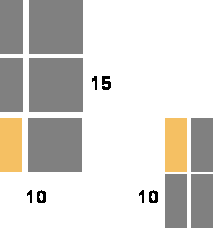
\includegraphics[width=0.4\columnwidth]{GA_get_example}
\par\end{center}


\section{Accumulate and Read-and-increment }

It is often useful in a put operation to combine the data moved to
the target process with the data that resides at that process, rather
then replacing the data there. \emph{Accumulate} and \emph{read\_inc}
perform an \emph{atomic} remote update to a patch (a section of the
global array) in the global array and an element in the global array,
respectively. They don't need the cooperation of the process(es) who
owns the data. Since the operations are atomic, the same portion of
a global array can be referenced by these operations issued by multiple
processes and the GA will assure the correct and consistent result
of the updates.

\emph{Accumulate} combines the data from the local array with data
in the global array section, which is
\begin{verbatim}
\textcolor{green}{n-D}~\textcolor{blue}{Fortran}~subroutine~\href{http://www.emsl.pnl.gov/docs/global/ga_ops.html\#ga_acc}{nga\_{}acc}(g\_a,~lo,~hi,~buf,~ld,~alpha)~

\textcolor{green}{2-D}~\textcolor{blue}{Fortran}~subroutine~\href{http://www.emsl.pnl.gov/docs/global/ga_ops.html\#ga_acc}{ga\_{}acc}(g\_a,~ilo,~ihi,~jlo,~jhi,~buf,~

~~~~~~~~~~~~~~~~~~~~~~~~~~~~~~ld,~alpha)~

\textcolor{blue}{C}~~~~~~~~~~~void~\href{http://www.emsl.pnl.gov/docs/global/c_nga_ops.html\#ga_acc}{NGA\_{}Acc}(int~g\_a,~int~lo{[}{]},~int~hi{[}{]},~void~{*}buf,~

~~~~~~~~~~~~~~~~~~~~~~~~~int~ld{[}{]},~void~{*}alpha)~

\textcolor{blue}{C++}~~~~~~~~~void~NGA::GlobalArray::acc(int~lo{[}{]},~int~hi{[}{]},~

~~~~~~~~~~~~~~~~~~~~~~~~~~~~~~~~~~~~~~~void~{*}buf,~int~ld{[}{]},~v

~~~~~~~~~~~~~~~~~~~~~~~~~~~~~~~~~~~~~~~oid~{*}alpha)
\end{verbatim}
The local array is assumed to have the same number of dimensions as
the global array. Users don't need to worry about where the region
defined by lo and hi is physically located. The function performs

\emph{global array section (lo{[}{]}, hi{[}{]})} += \emph{alpha {*}
buf}

Read\_inc remotely updates a particular element in the global array,
which is
\begin{verbatim}
\textcolor{green}{n-D}~\textcolor{blue}{Fortran}~subroutine~\href{http://www.emsl.pnl.gov/docs/global/ga_ops.html\#ga_read_inc}{nga\_{}read\_{}inc}(g\_a,~subscript,~inc)~

\textcolor{green}{2-D}~\textcolor{blue}{Fortran}~subroutine~\href{http://www.emsl.pnl.gov/docs/global/ga_ops.html\#ga_read_inc}{ga\_{}read\_{}inc}(g\_a,~i,~j,~inc)~

\textcolor{blue}{C}~~~~~~~~~~~long~\href{http://www.emsl.pnl.gov/docs/global/c_nga_ops.html\#ga_read_inc}{NGA\_{}Read\_{}inc}(int~g\_a,~int~subscript{[}{]},~long~inc)~

\textcolor{blue}{C++}~~~~~~~~~long~GA::GlobalArray::readInc(int~subscript{[}{]},~long~inc)
\end{verbatim}
This function applies to integer arrays only. It atomically reads
and increments an element in an integer array. It performs

\emph{a(subsripts)} += \emph{inc}

and returns the original value (before the update) of \emph{a(subscript)}. 


\section{Scatter/Gather }

\emph{Scatter} and \emph{gather} transfer a specified set of elements
to and from global arrays. They are one-sided: that is they don't
need the cooperation of the process(es) who own the referenced elements
in the global array.

Scatter puts array elements into a global array, which is
\begin{verbatim}
\textcolor{green}{n-D}~\textcolor{blue}{Fortran}~subroutine~\href{http://www.emsl.pnl.gov/docs/global/ga_ops.html\#ga_scatter}{nga\_{}scatter}(g\_a,~v,~subsarray,~n)~

\textcolor{green}{2-D}~\textcolor{blue}{Fortran}~subroutine~\href{http://www.emsl.pnl.gov/docs/global/ga_ops.html\#ga_scatter}{ga\_{}scatter}(g\_a,~v,~i,~j,~n)~

\textcolor{blue}{C}~~~~~~~~~~~void~\href{http://www.emsl.pnl.gov/docs/global/c_nga_ops.html\#ga_scatter}{NGA\_{}Scatter}(int~g\_a,~void~{*}v,~int~

~~~~~~~~~~~~~~~~~~~~~~~{*}subsarray{[}{]},~int~n)~

\textcolor{blue}{C++~}~~~~~~~~void~GA::GlobalArray::scatter(void~{*}v,~

~~~~~~~~~~~~~~~~~~~~~~~int~{*}subsarray{[}{]},~int~n)
\end{verbatim}
It performs (in C notation)
\begin{verbatim}
for(k=0;~k<=~n;~k++)~\{

a{[}subsArray{[}k{]}{[}0{]}{]}{[}subsArray{[}k{]}{[}1{]}{]}{[}subsArray{[}k{]}{[}2{]}{]}...~=~v{[}k{]};~

\}
\end{verbatim}
\emph{Example}:

Scatter the 5 elements into a 10x10 global array
\begin{verbatim}
Element~1~v{[}0{]}~=~5~subsArray{[}0{]}{[}0{]}~=~2~

~~~~~~~~~~~~~~~~~~~subsArray{[}0{]}{[}1{]}~=~3~

Element~2~v{[}1{]}~=~3~subsArray{[}1{]}{[}0{]}~=~3~

~~~~~~~~~~~~~~~~~~~subsArray{[}1{]}{[}1{]}~=~4~

Element~3~v{[}2{]}~=~8~subsArray{[}2{]}{[}0{]}~=~8~

~~~~~~~~~~~~~~~~~~~subsArray{[}2{]}{[}1{]}~=~5~

Element~4~v{[}3{]}~=~7~subsArray{[}3{]}{[}0{]}~=~3~

~~~~~~~~~~~~~~~~~~~subsArray{[}3{]}{[}1{]}~=~7~

Element~5~v{[}4{]}~=~2~subsArray{[}4{]}{[}0{]}~=~6~

~~~~~~~~~~~~~~~~~~~subsArray{[}4{]}{[}1{]}~=~3
\end{verbatim}
After the scatter operation, the five elements would be scattered
into the global array as shown in the following figure. 

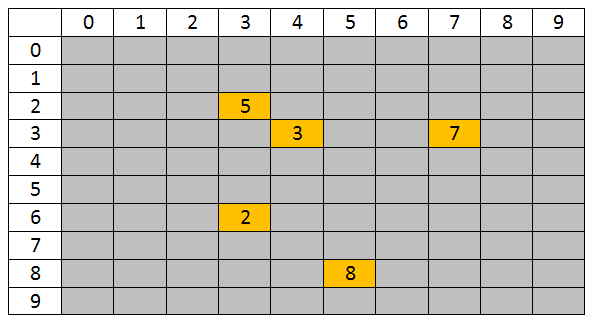
\includegraphics[scale=0.6]{scatter-GA}

\emph{Gather} is the reverse operation of scatter. It gets the array
elements from a global array into a local array.
\begin{verbatim}
\textcolor{green}{n-D}~\textcolor{blue}{Fortran}~subroutine~\href{http://www.emsl.pnl.gov/docs/global/ga_ops.html\#ga_gather}{nga\_{}gather}(g\_a,~v,~subsarray,~n)~

\textcolor{green}{2-D}~\textcolor{blue}{Fortran}~subroutine~\href{http://www.emsl.pnl.gov/docs/global/ga_ops.html\#ga_gather}{ga\_{}gather}ga\_gather(g\_a,~v,~i,~j,~n)~

\textcolor{blue}{C}~~~~~~~~~~~void~\href{http://www.emsl.pnl.gov/docs/global/c_nga_ops.html\#ga_gather}{NGA\_{}Gather}(int~g\_a,~void~{*}v,~

~~~~~~~~~~~~~~~~~~~~~~~~~~~~~int~{*}subsarray{[}{]},~int~n)~

\textcolor{blue}{C++}~~~~~~~~~void~GA::GlobalArray::gather(void~{*}v,~int~

~~~~~~~~~~~~~~~~~~~~~~~~~~~~~{*}subsarray{[}{]},~int~n)
\end{verbatim}
It performs (in C notation)
\begin{verbatim}
for(k=0;~k<=~n;~k++)\{~

~~~~~v{[}k{]}~=~a{[}subsArray{[}k{]}{[}0{]}{]}{[}subsArray{[}k{]}{[}1{]}{]}{[}subsArray{[}k{]}{[}2{]}{]}...;~

\}~
\end{verbatim}

\section{Periodic Interfaces }

Periodic interfaces to the one-sided operations have been added to
Global Arrays in version 3.1 to support some computational fluid dynamics
problems on multidimensional grids. They provide an index translation
layer that allows you to use put, get, and accumulate operations,
possibly extending beyond the boundaries of a global array. The references
that are outside of the boundaries are wrapped up inside the global
array. To better illustrate these operations, look at the following
example:

\emph{Example}: 

Assume a two dimensional global array g\_a with dimensions 5 X 5.

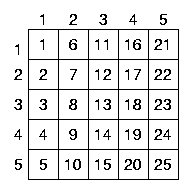
\includegraphics[width=7cm]{periodic1}

To access a patch {[}2:4,-1:3{]}, one can assume that the array is
wrapped over in the second dimension, as shown in the following figure 

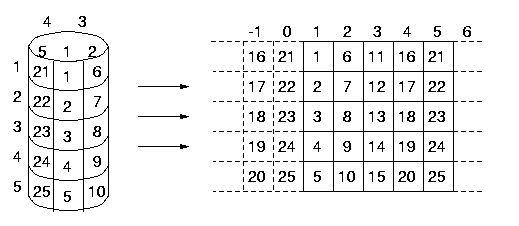
\includegraphics[scale=0.7]{periodic2}

Therefore the patch {[}2:4, -1:3{]} is
\begin{verbatim}
17~22~2~7~12~

18~23~3~8~13~

19~24~4~9~14
\end{verbatim}
Periodic operations extend the boudary of each dimension in two directions,
toward the lower bound and toward the upper bound. For any dimension
with lo(i) to hi(i), where 1 < i < ndim, it extends the range from 
\begin{verbatim}
{[}lo(i)~:~hi(i){]}~
\end{verbatim}
to 
\begin{verbatim}
{[}(lo(i)-1-(hi(i)-lo(i)+1))~:~(lo(i)-1){]},~{[}lo(i)~:~hi(i){]},~
\end{verbatim}
and 
\begin{verbatim}
{[}(hi(i)+1)~:~(hi(i)+1+(hi(i)-lo(i)+1)){]},~
\end{verbatim}
or 
\begin{verbatim}
{[}(lo(i)-1-(hi(i)-lo(i)+1))~:~(hi(i)+1+(hi(i)-lo(i)+1)){]}.
\end{verbatim}
Even though the patch spans in a much large range, the length must
always be less, or equal to (hi(i)-lo(i)+1)).

\emph{Example}: For a 2 x 2 array as shown in the following figure,
where the dimensions are {[}1:2, 1:2{]}, periodic operations would
look at the range of each of the dimensions as {[}-1:4, -1:4{]}.

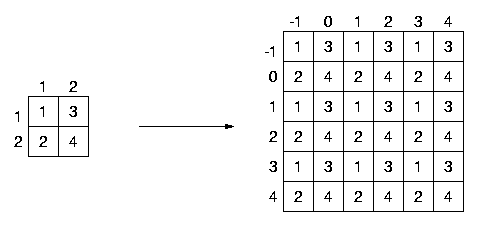
\includegraphics[scale=0.7]{periodic3}

Current version of GA supports three periodic operations. They are
\begin{itemize}
\item periodic get, 
\item periodic put, and 
\item periodic accumulate
\end{itemize}
\emph{Periodic Get }copies data from a global array section to a local
array, which is almost the same as regular get, except the indices
of the patch can be outside the boundaries of each dimension.
\begin{verbatim}
\textcolor{blue}{Fortran}~subroutine~\href{http://www.emsl.pnl.gov/docs/global/ga_ops.html\#ga_periodic_get}{nga\_{}periodic\_{}get}(g\_a,~lo,~hi,~buf,~ld)~

\textcolor{blue}{C}~~~~~~~void~\href{http://www.emsl.pnl.gov/docs/global/c_nga_ops.html\#ga_periodic_get}{NGA\_{}Periodic\_{}get}(int~g\_a,~int~lo{[}{]},~int~hi{[}{]},~

~~~~~~~~~~~~~void~{*}buf,~int~ld{[}{]})~

\textcolor{blue}{C++}~~~~~void~GA::GlobalArray::periodicGet(int~lo{[}{]},~

~~~~~~~~~~~~~int~hi{[}{]},~void~{*}buf,~int~ld{[}{]})
\end{verbatim}
Similar to regular \emph{get}, \texttt{\emph{lo}} and \texttt{\emph{hi}}
specify where the data should come from in the global array, and \texttt{\emph{ld}}
specifies the stride information of the local array \texttt{\emph{buf}}.

\emph{Example}: Let us look at the first example in this section.
It is 5 x 5 two dimensional global array. Assume that the local buffer
is an 4x3 array. 

Also assume that
\begin{verbatim}
1o{[}0{]}~=~-1,~hi{[}0{]}~=~2,~

lo{[}1{]}~=~4,~hi{[}1{]}~=~6,~and~

ld{[}0{]}~=~4.
\end{verbatim}
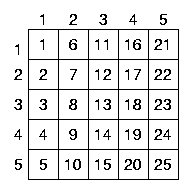
\includegraphics[width=7cm]{periodic1}

The local buffer \texttt{\emph{buf}} is
\begin{verbatim}
19~~~~24~~~~4~

20~~~~25~~~~5~~

16~~~~21~~~~1~

17~~~~22~~~~2~
\end{verbatim}
Periodic Put is the reverse operations of Periodic Get. It copies
data from the local array to the global array section, which is
\begin{verbatim}
\textcolor{blue}{Fortran}~subroutine~\href{http://www.emsl.pnl.gov/docs/global/ga_ops.html\#ga_periodic_put}{nga\_{}periodic\_{}put}(g\_a,~lo,~hi,~buf,~ld)~

\textcolor{blue}{C}~~~~~~~void~\href{http://www.emsl.pnl.gov/docs/global/c_nga_ops.html\#ga_periodic_put}{NGA\_{}Periodic\_{}put}(int~g\_a,~int~lo{[}{]},~int~hi{[}{]},~

~~~~~~~~~~~~~void~{*}buf,~int~ld{[}{]})~

\textcolor{blue}{C++}~~~~~void~GA::GlobalArray::periodicPut(int~lo{[}{]},~

~~~~~~~~~~~~~int~hi{[}{]},~void~{*}buf,~int~ld{[}{]})
\end{verbatim}
Similar to regular\emph{ put}, \texttt{\emph{lo}} and \texttt{\emph{hi}}
specify where the data should go in the global array; \texttt{\emph{ld}}
specifies the stride information of the local array \texttt{\emph{buf}}.

\emph{Periodic Put/Get} (also include the \emph{Accumulate}, which
will be discussed later in this section) divide the patch into several
smaller patches. For those smaller patches that are outside the global
aray, adjust the indices so that they rotate back to the original
array. After that call the regular \emph{Put/Get/Accumulate}, for
each patch, to complete the operations.

\emph{Example}: Look at the example for periodic get. Because it is
a 5 x 5 global array, the valid indices for each dimension are
\begin{verbatim}
dimension~0:~{[}1~:~5{]}~

dimension~1:~{[}1~:~5{]}
\end{verbatim}
The specified lo and hi are apparently out of the range of each dimension:
\begin{verbatim}
dimemsion~0:~{[}-1~:~2{]}~-{}->~{[}-1~:~0{]}~-{}-~wrap~back~-{}->~{[}4~:~5{]}~{[}~1~:~2{]}~ok

dimension~1:~{[}~4~:~6{]}~-{}->~{[}~4~:~5{]}~ok~{[}~6~:~6{]}~-{}-~wrap~back~-{}->~{[}1~:~1{]}
\end{verbatim}
Hence, there will be four smaller patches after the adjustment. They
are
\begin{verbatim}
patch~0:~{[}4~:~5,~4~:~5{]}~

patch~1:~{[}4~:~5,~1~:~1{]}~

patch~2:~{[}1~:~2,~4~:~5{]}~

patch~3:~{[}1~:~2,~1~:~1{]}
\end{verbatim}
as shown in the following figure

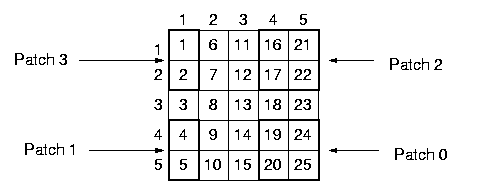
\includegraphics[width=0.7\paperwidth]{periodic4}

Of course the destination addresses of each samller patch in the local
buffer also need to be calculated.

Similar to regular \emph{Accumulate, Periodic Accumulate} combines
the data from the local array with data in the global array section,
which is
\begin{verbatim}
\textcolor{blue}{Fortran}~subroutine~\href{http://www.emsl.pnl.gov/docs/global/ga_ops.html\#ga_periodic_acc}{nga\_{}periodic\_{}acc}(g\_a,~lo,~hi,~buf,~ld,~alpha)~

\textcolor{blue}{C}~~~~~~~void~\href{http://www.emsl.pnl.gov/docs/global/c_nga_ops.html\#ga_periodic_acc}{NGA\_{}Periodic\_{}acc}(int~g\_a,~int~lo{[}{]},~int~hi{[}{]},~

~~~~~~~~~~~~~~~~~~~void~{*}buf,~int~ld{[}{]},~void~{*}alpha)~

\textcolor{blue}{C++~}~~~~void~GA::GlobalArray::periodicAcc(int~lo{[}{]},~int~hi{[}{]},~

~~~~~~~~~~~~~~~~~~~void~{*}buf,~int~ld{[}{]},~void~{*}alpha)
\end{verbatim}
The local array is assumed to have the same number of dimensions as
the global array. Users don't need to worry about where the region
defined by \texttt{\emph{lo}} and \texttt{\emph{hi}} is physically
located. The function performs

\emph{global array section (lo{[}{]}, hi{[}{]}) += alpha {*} buf}

\emph{Example}: Let us look at the same example as above. There is
a 5 x 5 two dimensional global array. Assume that the local buffer
is an 4x3 array. 

Also assume that
\begin{verbatim}
1o{[}0{]}~=~-1,~hi{[}0{]}~=~2,~

lo{[}1{]}~=~4,~hi{[}1{]}~=~6,~and~

ld{[}0{]}~=~4.
\end{verbatim}
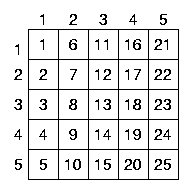
\includegraphics[width=7cm]{periodic1}

The local buffer buf is
\begin{verbatim}
1~~5~~9~

4~~6~~5~

3~~2~~1~

7~~8~~2
\end{verbatim}
and the \texttt{\emph{alpha = 2}}.

After the Periodic Accumulate operation, the global array will be

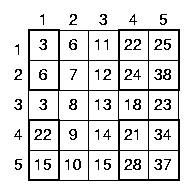
\includegraphics[width=7cm]{periodic5}


\section{Non-blocking operations}

The non-blocking operations (get/put/accumulate) are derived from
the blocking interface by adding a handle argument that identifies
an instance of the non-blocking request. Nonblocking operations initiate
a communication call and then return control to the application. A
return from a nonblocking operation call indicates a mere initiation
of the data transfer process and the operation can be completed locally
by making a call to the wait (e.g. nga\_nbwait) routine.

The wait function completes a non-blocking one-sided operation locally.
Waiting on a nonblocking put or an accumulate operation assures that
data was injected into the network and the user buffer can be now
be reused. Completing a get operation assures data has arrived into
the user memory and is ready for use. Wait operation ensures only
local completion. Unlike their blocking counterparts, the nonblocking
operations are not ordered with respect to the destination. Performance
being one reason, the other reason is that by ensuring ordering we
incur additional and possibly unnecessary overhead on applications
that do not require their operations to be ordered. For cases where
ordering is necessary, it can be done by calling a fence operation.
The fence operation is provided to the user to confirm remote completion
if needed.

\begin{tabular}{|>{\raggedright}p{13cm}|}
\hline 
\emph{Example}: Let us take a simple case for illustration. Say, there
are two global arrays i.e. one array stores pressure and the other
stores temperature. If there are two computation phases (first phase
computes pressure and second phase computes temperature), then we
can overlap communication with computation, thus hiding latency.\tabularnewline
\hline 
\begin{verbatim}
.~.~.~.~.~.~.~.~.~

nga\_get~(get\_pressure\_array)

nga\_nbget(initiates~data~transfer~to~get~temperature\_array,~

~~~~~and~returns~immediately)

compute\_pressure()~/{*}~hiding~latency~-~communication~

~~~~~is~overlapped~with~computation~{*}/

nga\_nbwait(temperature\_array~-~completes~data~transfer)

compute\_temperature()~

.~.~.~.~.~.~.~.
\end{verbatim}
\tabularnewline
\hline
\end{tabular}

The non-blocking APIs are derived from the blocking interface by adding
a handle argument that identifies an instance of the non-blocking
request.
\begin{verbatim}
\textcolor{green}{n-D}~\textcolor{blue}{Fortran}~subroutine~\href{http://www.emsl.pnl.gov/docs/global/ga_ops.html\#nga_nbput}{nga\_{}nbput}(g\_a,~lo,~hi,~buf,~ld,~nbhandle)~

\textcolor{green}{n-D}~Fortran~subroutine~\href{http://www.emsl.pnl.gov/docs/global/ga_ops.html\#nga_nbget}{nga\_{}nbget}(g\_a,~lo,~hi,~buf,~ld,~nbhandle)~

\textcolor{green}{n-D}~\textcolor{blue}{Fortran}~subroutine~\href{http://www.emsl.pnl.gov/docs/global/ga_ops.html\#nga_nbacc}{nga\_{}nbacc}(g\_a,~lo,~hi,~buf,~ld,~alpha,~

~~~~~~~~~~~~~~~~~~~~~nbhandle)~

\textcolor{green}{n-D}~\textcolor{blue}{Fortran}~subroutine~\href{http://www.emsl.pnl.gov/docs/global/ga_ops.html\#nga_nbwait}{nga\_{}nbwait}(nbhandle)

\textcolor{green}{2-D}~\textcolor{blue}{Fortran}~subroutine~\href{http://www.emsl.pnl.gov/docs/global/ga_ops.html\#ga_nbput}{ga\_{}nbput}(g\_a,~ilo,~ihi,~jlo,~jhi,~buf,

~~~~~~~~~~~~~~~~~~~~~ld,~nbhandle)~

\textcolor{green}{2-D}~\textcolor{blue}{Fortran}~subroutine~\href{http://www.emsl.pnl.gov/docs/global/ga_ops.html\#ga_nbget}{ga\_{}nbget}(g\_a,~ilo,~ihi,~jlo,~jhi,~buf,~

~~~~~~~~~~~~ld,~nbhandle)~

\textcolor{green}{2-D}~\textcolor{blue}{Fortran}~subroutine~\href{http://www.emsl.pnl.gov/docs/global/ga_ops.html\#ga_nbacc}{ga\_{}nbacc}(g\_a,~ilo,~ihi,~jlo,~jhi,~buf,~

~~~~~~~~~~~~ld,~alpha,~nbhandle)~

\textcolor{green}{2-D}~\textcolor{blue}{Fortran}~subroutine~\href{http://www.emsl.pnl.gov/docs/global/ga_ops.html\#ga_nbwait}{ga\_{}nbwait}(nbhandle)

\textcolor{blue}{C}~~~~~~~~~~~void~\href{http://www.emsl.pnl.gov/docs/global/c_nga_ops.html\#ga_nbput}{NGA\_{}NbPut}(int~g\_a,~int~lo{[}{]},~int~hi{[}{]},~

~~~~~~~~~~~~~~~~~~~~~void~{*}buf,~int~ld{[}{]},~ga\_nbhdl\_t{*}~nbhandle)~

\textcolor{blue}{C}~~~~~~~~~~~void~\href{http://www.emsl.pnl.gov/docs/global/c_nga_ops.html\#ga_nbget}{NGA\_{}NbGet}(int~g\_a,~int~lo{[}{]},~int~hi{[}{]},~

~~~~~~~~~~~~~~~~~~~~~void~{*}buf,~int~ld{[}{]},~ga\_nbhdl\_t{*}~nbhandle)~

\textcolor{blue}{C}~~~~~~~~~~~void~\href{http://www.emsl.pnl.gov/docs/global/c_nga_ops.html\#ga_nbacc}{NGA\_{}NbAcc}(int~g\_a,~int~lo{[}{]},~int~hi{[}{]},~

~~~~~~~~~~~~~~~~~~~~~void~{*}buf,~int~ld{[}{]},~void~{*}alpha,~

~~~~~~~~~~~~~~~~~~~~~ga\_nbhdl\_t{*}~nbhandle)~

\textcolor{blue}{C}~~~~~~~~~~~int~\href{http://www.emsl.pnl.gov/docs/global/c_nga_ops.html\#ga_nbwait}{NGA\_{}NbWait}(ga\_nbhdl\_t{*}~nbhandle)

\textcolor{blue}{C++}~~~~~~~~~void~GA::GlobalArray::nbPut(int~lo{[}{]},~int~hi{[}{]},~

~~~~~~~~~~~~~~~~~~~~~~~~~~~~~~~~~~~~~~~~void~{*}buf,~

~~~~~~~~~~~~~int~ld{[}{]},~ga\_nbhdl\_t{*}~nbhandle)~

\textcolor{blue}{C++}~~~~~~~~~void~GA::GlobalArray::nbGet(int~lo{[}{]},~int~hi{[}{]},~

~~~~~~~~~~~~~~~~~~~~~~~~~~~~~~~~~~~~~~~void~{*}buf,~

~~~~~~~~~~~~~int~ld{[}{]},~ga\_nbhdl\_t{*}~nbhandle)~

\textcolor{blue}{C++}~~~~~~~~~void~GA::GlobalArray::nbAcc(int~lo{[}{]},~int~hi{[}{]},~

~~~~~~~~~~~~~~~~~~~~~~~~~~~~~~~~~~~~~~~void~{*}buf,~

~~~~~~~~~~~~~int~ld{[}{]},~void~{*}alpha,~ga\_nbhdl\_t{*}~nbhandle)~

\textcolor{blue}{C++}~~~~~~~~~int~GA::GlobalArray::NbWait(ga\_nbhdl\_t{*}~nbhandle)
\end{verbatim}



\chapter{Interprocess Synchronization}

\chapter{Interprocess Synchronization}

Global Arrays provide three types of synchronization calls to support
different synchronization styles. 

\begin{tabular}{|>{\centering}p{3cm}|>{\raggedright}p{6cm}|}
\hline 
\emph{Lock with mutex:}  & is useful for a shared memory model. One can lock a mutex, to exclusively
access a critical section. \tabularnewline
\hline 
\emph{Fence:}  & guarantees that the Global Array operations issued from the calling
process are complete. The fence operation is local. \tabularnewline
\hline 
\emph{Sync:}  & is a barrier. It synchronizes processes and ensures that all Global
Array operations are completed. Sync operation is collective. \tabularnewline
\hline
\end{tabular}


\section{Lock and Mutex }

Lock works together with mutex. It is a simple synchronization mechanism
used to protect a critical section.To enter a critical section, typically,
one needs to do:
\begin{verbatim}
1.~~Create~mutexes~

2.~~Lock~on~a~mutex~

3.~~...~

~~~~Do~the~exclusive~operation~in~the~critical~section~~

~~~~...~

4.~~Unlock~the~mutex~

5.~~Destroy~mutexes
\end{verbatim}
The function
\begin{verbatim}
\textcolor{blue}{Fortran}~logical~function~\href{http://www.emsl.pnl.gov/docs/global/ga_ops.html\#ga_create_mutex}{ga\_{}create\_{}mutexes}(number)~

\textcolor{blue}{C}~~~~~~~int~\href{http://www.emsl.pnl.gov/docs/global/c_nga_ops.html\#ga_create_mutexes}{GA\_{}Create\_{}mutexes}(int~number)~

\textcolor{blue}{C++~}~~~~int~GA::GAServices::createMutexes(int~number)
\end{verbatim}
creates a set containing the number of mutexes. Only one set of mutexes
can exist at a time. Mutexes can be created and destroyed as many
times as needed. Mutexes are numbered: 0, ..., number-1.

The function
\begin{verbatim}
\textcolor{blue}{Fortran}~logical~function~\href{http://www.emsl.pnl.gov/docs/global/ga_ops.html\#ga_destroy_mutex}{ga\_{}destroy\_{}mutexes}()~

\textcolor{blue}{C}~~~~~~~int~\href{http://www.emsl.pnl.gov/docs/global/c_nga_ops.html\#ga_destroy_mutexes}{GA\_{}Destroy\_{}mutexes}()

\textcolor{blue}{C++}~~~~~int~GA::GAServices::destroyMutexes()
\end{verbatim}
destroys the set of mutexes created with ga\_create\_mutexes.

Both \texttt{\emph{ga\_create\_mutexes}} and \texttt{\emph{ga\_destroy\_mutexes}}
are collective operations.

The functions
\begin{verbatim}
\textcolor{blue}{Fortran}~subroutine~\href{http://www.emsl.pnl.gov/docs/global/ga_ops.html\#ga_lock}{ga\_{}lock}(int~mutex)~

~~~~~~~~subroutine~\href{http://www.emsl.pnl.gov/docs/global/ga_ops.html\#ga_unlock}{ga\_{}unlock}(int~mutex)~

\textcolor{blue}{C}~~~~~~~void~\href{http://www.emsl.pnl.gov/docs/global/c_nga_ops.html\#ga_lock}{GA\_{}lock}(int~mutex)~

~~~~~~~~void~\href{http://www.emsl.pnl.gov/docs/global/c_nga_ops.html\#ga_unlock}{GA\_{}unlock}(int~mutex)~

\textcolor{blue}{C++}~~~~~void~GA::GAServices::lock(int~mutex)~

~~~~~~~~void~GA::GAServices::unlock(int~mutex)
\end{verbatim}
lock and unlock a mutex object identified by the mutex number, respectively.
It is a fatal error for a process to attempt to lock a mutex which
has already been locked by this process, or unlock a mutex which has
not been locked by this process.

\emph{\underbar{Example}}\underbar{ }\emph{\underbar{1}}\underbar{:}

Use one mutex and the lock mechanism to enter the critical section.
\begin{verbatim}
status~=~ga\_create\_mutexes(1)~

if(.not.status)~then~

~~~call~ga\_error('ga\_create\_mutexes~failed~',0)~

endif~

call~ga\_lock(0)

~~~...~do~something~in~the~critical~section~

call~ga\_put(g\_a,~...)~

~~~...

call~ga\_unlock(0)~

if(.not.ga\_destroy\_mutexes())~then~

~~~call~ga\_error('mutex~not~destroyed',0)~
\end{verbatim}

\section{Fence }

Fence blocks the calling process until all the data transfers corresponding
to the Global Array operations initiated by this process complete.
The typical scenario that it is being used is
\begin{verbatim}
1.~~Initialize~the~fence~

2.~~...~

~~~~~~~~Global~array~operations~

~~~~...~

3.~~Fence
\end{verbatim}
This would guarantee the operations between step 1 and 3 are complete.

The function
\begin{verbatim}
\textcolor{blue}{Fortran}~subroutine~\href{http://www.emsl.pnl.gov/docs/global/ga_ops.html\#ga_init_fence}{ga\_{}init\_{}fence}()~

\textcolor{blue}{C}~~~~~~~void~\href{http://www.emsl.pnl.gov/docs/global/c_nga_ops.html\#ga_init_fence}{GA\_{}Init\_{}fence}()~

\textcolor{blue}{C++}~~~~~void~GA::GAServices::initFence()
\end{verbatim}
Initializes tracing of completion status of data movement operations.

The function
\begin{verbatim}
\textcolor{blue}{Fortran}~subroutine~\href{http://www.emsl.pnl.gov/docs/global/ga_ops.html\#ga_fence}{ga\_{}fence}()~

\textcolor{blue}{C}\textcolor{blue}{\underbar{~}}~~~~~~void~\href{http://www.emsl.pnl.gov/docs/global/c_nga_ops.html\#ga_fence}{GA\_{}Fence}()~

\textcolor{blue}{C++}~~~~~void~GA::GAServices::fence()
\end{verbatim}
blocks the calling process until all the data transfers corresponding
to GA operations called after \texttt{\emph{ga\_init\_fence}} complete.

\texttt{\emph{ga\_fence}} must be called after \texttt{\emph{ga\_init\_fence}}.
A barrier, \texttt{\emph{ga\_sync}}, assures completion of all data
transfers and implicitly cancels outstanding ga\_init\_fence. \texttt{\emph{ga\_init\_fence}}
and \texttt{\emph{ga\_fence}} must be used in pairs, multiple calls
to \texttt{\emph{ga\_fence}} require the same number of corresponding
\texttt{\emph{ga\_init\_fence}} calls. \texttt{\emph{ga\_init\_fence/ga\_fence}}
pairs can be nested.

\textit{\underbar{Example 1:}}

Since \texttt{\emph{ga\_put}} might return before the data reaches
the final destination \texttt{\emph{ga\_init\_fence}} and \texttt{\emph{ga\_fence}}
allow the process to wait until the data is actually moved:
\begin{verbatim}
call~ga\_init\_fence()~

call~ga\_put(g\_a,~...)~

call~ga\_fence()
\end{verbatim}
\textit{\underbar{Example 2:}}

\texttt{\emph{ga\_fence}} works for multiple GA operations.
\begin{verbatim}
call~ga\_init\_fence()~

call~ga\_put(g\_a,~...)~

call~ga\_scatter(g\_a,~...)~

call~ga\_put(g\_b,~...)~

call~ga\_fence()
\end{verbatim}
The calling process will be blocked until data movements initiated
by two calls to \texttt{ga\_put} and one \texttt{ga\_scatter} complete. 


\section{Sync }

Sync is a collective operation. It acts as a barrier, which synchronizes
all the processes and ensures that all the Global Array operations
are complete at the call.

The function is
\begin{verbatim}
\textcolor{blue}{Fortran}~subroutine~\href{http://www.emsl.pnl.gov/docs/global/ga_ops.html\#ga_sync}{ga\_{}sync}()~

\textcolor{blue}{C}~~~~~~~void~\href{http://www.emsl.pnl.gov/docs/global/c_nga_ops.html\#ga_sync}{GA\_{}Sync}()~

\textcolor{blue}{C++}~~~~~void~GA::GAServices::sync()
\end{verbatim}
Sync should be inserted as necessary. With many sync calls, the application
performance would suffer. 


\chapter{Collective Array Operations}

\chapter{Collective Array Operations}

Global Arrays provide functions for collective array operations, targeting
both whole arrays and patches (portions of global arrays). Collective
operations require all the processes to make the call. In the underlying
implementation, each process deals with its local data. These functions
include:
\begin{itemize}
\item basic array operations, 
\item linear algebra operations, and 
\item interfaces to third party software packages.
\end{itemize}

\section{Basic Array Operations }

Global Arrays provide several mechanisms to manipulate contents of
the arrays. One can set all the elements in an array/patch to a specific
value, or as a special case set to zero. Since GA does not explicitly
initialize newly created arrays, these calls are useful for initialization
of an array/patch. (To fill the array with different values for each
element, one can choose the one sided operation putor each process
can initialize its local portion of an array/patch like ordinary local
memory). One can also scale the array/patch by a certain factor, or
copy the contents of one array/patch to another. 


\subsection{Whole Arrays }

These functions apply to the entire array.

The function
\begin{verbatim}
\textcolor{blue}{Fortran}~subroutine~\href{http://www.emsl.pnl.gov/docs/global/ga_ops.html\#ga_zero}{ga\_{}zero}(g\_a)~

\textcolor{blue}{C}~~~~~~~void~\href{http://www.emsl.pnl.gov/docs/global/c_nga_ops.html\#ga_zero}{GA\_{}Zero}(int~g\_a)~

\textcolor{blue}{C++}~~~~~void~GA::GlobalArray::zero()
\end{verbatim}
sets all the elements in the array to zero.

To assign a single value to all the elements in an array, use the
function
\begin{verbatim}
\textcolor{blue}{Fortran}~subroutine~\href{http://www.emsl.pnl.gov/docs/global/ga_ops.html\#ga_fill}{ga\_{}fill}(g\_a,~val)~

\textcolor{blue}{C}~~~~~~~void~\href{http://www.emsl.pnl.gov/docs/global/c_nga_ops.html\#ga_fill}{GA\_{}Fill}(int~g\_a,~void~{*}val)~

\textcolor{blue}{C++}~~~~~void~GA::GlobalArray::fill(void~{*}val)
\end{verbatim}
It sets all the elements in the array to the value \emph{val}. The
\emph{val} must have the same data type as that of the array.

The function
\begin{verbatim}
\textcolor{blue}{Fortran}~subroutine~\href{http://www.emsl.pnl.gov/docs/global/ga_ops.html\#ga_scale}{ga\_{}scale}(g\_a,~val)~

\textcolor{blue}{C}~~~~~~~void~\href{http://www.emsl.pnl.gov/docs/global/c_nga_ops.html\#ga_scale}{GA\_{}scale}(int~g\_a,~void~{*}val)~

\textcolor{blue}{C++}~~~~~void~GA::GlobalArray::scale(void~{*}val)
\end{verbatim}
scales all the elements in the array by factor \emph{val}. Again the
val must be the same data type as that of the array itself.

The above three functions are dealing with one global array, to set
values or change all the elements together. The following functions
are for copying data between two arrays.

The function
\begin{verbatim}
\textcolor{blue}{Fortran}~subroutine~\href{http://www.emsl.pnl.gov/docs/global/ga_ops.html\#ga_copy}{ga\_{}copy}(g\_a,~g\_b)~

\textcolor{blue}{C}~~~~~~~void~\href{http://www.emsl.pnl.gov/docs/global/c_nga_ops.html\#ga_copy}{GA\_{}copy}(int~g\_a,~int~g\_b)~

\textcolor{blue}{C++}~~~~~void~GA::GlobalArray::copy

~~~~~~~~~~~~~(const~GA::GlobalArray~{*}~g\_a)
\end{verbatim}
copies the contents of one array to another. The arrays must be of
the same data type and have the same number of elements.

For global arrays containing ghost cells, the ghost cell data can
be filled in with the corresponding data from neighboring processors
using the command
\begin{verbatim}
\textcolor{blue}{n-d~Fortran}~subroutine~\href{http://www.emsl.pnl.gov/docs/global/ga_ops.html\#ga_copy}{ga\_{}copy}(g\_a,~g\_b)~

\textcolor{blue}{C~}~~~~~~~~~~void~\href{http://www.emsl.pnl.gov/docs/global/c_nga_ops.html\#ga_copy}{GA\_{}copy}(int~g\_a,~int~g\_b)~

\textcolor{blue}{C++}~~~~~~~~~void~GA::GlobalArray::

~~~~~~~~~~~~~~~~~~copy(const~GA::GlobalArray~{*}~g\_a)



\textcolor{blue}{n-d~Fortran}~subroutine~\href{http://www.emsl.pnl.gov/docs/global/ga_ops.html\#ga_update_ghosts}{ga\_{}update\_{}ghosts}(g\_a)~

\textcolor{blue}{C}~~~~~~~~~~~void~\href{http://www.emsl.pnl.gov/docs/global/c_nga_ops.html\#ga_update_ghosts}{ga\_{}update\_{}ghosts}(int~g\_a)~

\textcolor{blue}{C++}~~~~~~~~~void~GA::GlobalArray::updateGhosts()~
\end{verbatim}
This operation updates the ghost cell data by assuming periodic, or
wrap-around, boundary conditions similar to those described for the\texttt{
nga\_periodic\_get} operations described above. The wrap-around conditions
are always applied, it is up to the individual application to decide
whether or not the data in the ghost cells should be used. The update
operation is illustrated below for a simple 4x2 global array distributed
across two processors. The ghost cells are one element wide in each
dimension.

\begin{tabular}{|c|}
\hline 
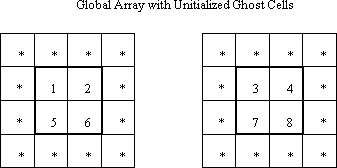
\includegraphics[width=10cm]{ghost012}\tabularnewline
\hline
\hline 
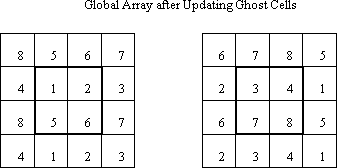
\includegraphics[width=10cm]{ghost015}\tabularnewline
\hline
\end{tabular}
\begin{verbatim}
\textcolor{blue}{n-d~Fortran}~logical~function~\href{http://www.emsl.pnl.gov/docs/global/ga_ops.html\#ga_update_ghost_dir}{nga\_{}update\_{}ghosts\_{}dir}(g\_a,~

~~~~~~~~~~~~~~~~~~~~~~~~dimension,~idir,~flag)~

\textcolor{blue}{C}~~~~~~~~~~~int~\href{http://www.emsl.pnl.gov/docs/global/c_nga_ops.html\#nga_update_ghost_dir}{NGA\_{}Update\_{}ghosts\_{}dir}(int~g\_a,~int~

~~~~~~~~~~~~~~~~~~~~~~~~dimension,~int~idir,~int~cflag)~

\textcolor{blue}{C++}~~~~~~~~~int~GA::GlobalArray::updateGhostsDir

~~~~~~~~~~~~~~~~~~~~~~~(int~dimension,~int~idir,~int~cflag)~
\end{verbatim}
This function can be used to update the ghost cells along individual
directions.

It is designed for algorithms that can overlap updates with computation.
The variable dimension indicates which coordinate direction is to
be updated (e.g. dimension = 1 would correspond to the y axis in a
two or three dimensional system), the variable idir can take the values
+/-1 and indicates whether the side that is to be updated lies in
the positive or negative direction, and cflag indicates whether or
not the corners on the side being updated are to be included in the
update. The following calls would be equivalent to a call to \texttt{GA\_Update\_ghosts}
for a 2-dimensional system:
\begin{verbatim}
status~=~NGA\_Update\_ghost\_dir(g\_a,0,-1,1);~

status~=~NGA\_Update\_ghost\_dir(g\_a,0,1,1);~

status~=~NGA\_Update\_ghost\_dir(g\_a,1,-1,0);~

status~=~NGA\_Update\_ghost\_dir(g\_a,1,1,0);
\end{verbatim}
The variable \emph{cflag} is set equal to 1 (or non-zero) in the first
two calls so that the corner ghost cells are update, it is set equal
to 0 in the second two calls to avoid redundant updates of the corners.
Note that updating the ghosts cells using several independent calls
to the \texttt{nga\_update\_ghost\_dir} functions is generally not
as efficient as using \texttt{GA\_Update\_ghosts} unless the individual
calls can be effectively overlapped with computation. This is a collective
operation. 


\subsection{Patches }

GA provides a set of operations on segments of the global arrays,
namely patch operations. These functions are more general, in a sense
they can apply to the entire array(s). As a matter of fact, many of
the Global Array collective operations are based on the patch operations,
for instance, the \texttt{GA\_Printis} only a special case of \texttt{NGA\_Print\_patch},
called by setting the bounds of the patch to the entire global array.
There are two interfaces for Fortran, one for two dimensional and
the other for n-dimensional (one to seven). The (n-dimensional) interface
can surely handle the two dimensional case as well. It is available
for backward compatibility purposes. The functions dealing with n-dimensional
patches use the \textquotedbl{}\texttt{nga}\textquotedbl{}prefix and
those dealing with two dimensional patches start with the \textquotedbl{}\texttt{ga}\textquotedbl{}
prefix.

The function
\begin{verbatim}
\textcolor{blue}{Fortran}~subroutine~\href{http://www.emsl.pnl.gov/docs/global/ga_ops.html\#ga_zero_patch}{nga\_{}zero\_{}patch}nga\_zero\_patch(g\_a,~alo,~ahi)~

\textcolor{blue}{C}~~~~~~~void~\href{http://www.emsl.pnl.gov/docs/global/c_nga_ops.html\#ga_zero_patch}{NGA\_{}Zero\_{}patch}(int~g\_a,~int~lo{[}{]}~int~hi{[}{]})~

\textcolor{blue}{C++}~~~~~void~GA::GlobalArray::zeroPatch(int~lo{[}{]}~int~hi{[}{]})
\end{verbatim}
is similar to \emph{ga\_zero}, except that instead of applying to
entire array, it sets only the region defined by \emph{lo} and \emph{hi}
to zero.

One can assign a single value to all the elements in a patch with
the function:
\begin{verbatim}
\textcolor{green}{n-D}\textcolor{blue}{Fortran}~subroutine~\href{http://www.emsl.pnl.gov/docs/global/ga_ops.html\#ga_fill_patch}{nga\_{}fill\_{}patch}(g\_a,~lo,~hi,~val)~

\textcolor{green}{2-D}\textcolor{blue}{Fortran}~subroutine~\href{http://www.emsl.pnl.gov/docs/global/ga_ops.html\#ga_fill_patch}{ga\_{}fill\_{}patch}(g\_a,~ilo,~ihi,~

~~~~~~~~~~~~~~~~~~~jlo,~jhi,~val)~

\textcolor{blue}{C}~~~~~~~~~~void~\href{http://www.emsl.pnl.gov/docs/global/c_nga_ops.html\#ga_fill_patch}{NGA\_{}Fill\_{}patch}(int~g\_a,~int~lo{[}{]}~

~~~~~~~~~~~~~~~~~~~int~hi{[}{]},~void~{*}val)~

\textcolor{blue}{C++}~~~~~~~~void~GA::GlobalArray::fillPatch(int~lo{[}{]}~

~~~~~~~~~~~~~~~~~~~int~hi{[}{]},~void~{*}val)
\end{verbatim}
The\texttt{ lo} and \texttt{hi} defines the patch and the \texttt{val}
is the value to set.

The function
\begin{verbatim}
\textcolor{green}{n-D}\textcolor{blue}{Fortran}~subroutine~\href{http://www.emsl.pnl.gov/docs/global/ga_ops.html\#ga_scale_patch}{nga\_{}scale\_{}patch}(g\_a,~lo,~hi,~val)~

\textcolor{green}{2-D}\textcolor{blue}{Fortran}~subroutine~\href{http://www.emsl.pnl.gov/docs/global/ga_ops.html\#ga_scale_patch}{ga\_{}scale\_{}patch}(g\_a,~ilo,~ihi,~jlo,~

~~~~~~~~~~~~~~~~~~jhi,~val)~

\textcolor{blue}{C}~~~~~~~~~~void~\href{http://www.emsl.pnl.gov/docs/global/c_nga_ops.html\#ga_scale_patch}{NGA\_{}Scale\_{}patch}(int~g\_a,~int~lo{[}{]}~int~

~~~~~~~~~~~~~~~~~~hi{[}{]},~void~{*}val)~

\textcolor{blue}{C++}~~~~~~~~void~GA::GlobalArray::scalePatch(int~lo{[}{]}~

~~~~~~~~~~~~~~~~~~int~hi{[}{]},~void~{*}val)
\end{verbatim}
scales the patch defined by \texttt{lo }and \texttt{hi} by the factor
\texttt{val}.

The copy patch operation is one of the fundamental and frequently
used functions. The function
\begin{verbatim}
\textcolor{green}{n-D}\textcolor{blue}{Fortran}~subroutine~\href{http://www.emsl.pnl.gov/docs/global/ga_ops.html\#ga_copy_patch}{nga\_{}copy\_{}patch}(trans,~g\_a,~alo,~

~~~~~~~~~~~~~~~~~~~~~~ahi,~g\_b,~blo,~bhi)~

\textcolor{green}{2-D}\textcolor{blue}{Fortran}~subroutine~\href{http://www.emsl.pnl.gov/docs/global/ga_ops.html\#ga_copy_patch}{ga\_{}copy\_{}patch}(trans,~g\_a,~ailo,~

~~~~~~~~~~~~~~~~~~~~~~aihi,~ajlo,~ajhi,~g\_b,~bilo,~bihi,~

~~~~~~~~~~~~~~~~~~~~~~bjlo,~bjhi)~

\textcolor{blue}{C~}~~~~~~~~~void~\href{http://www.emsl.pnl.gov/docs/global/c_nga_ops.html\#ga_copy_patch}{NGA\_{}Copy\_{}patch}(char~trans,~int~g\_a~,~

~~~~~~~~~~~~~~~~~~~~~~int~alo{[}{]},~int~ahi{[}{]},~int~g\_b,~

~~~~~~~~~~~~~~~~~~~~~~int~blo{[}{]},~int~bhi{[}{]})~

\textcolor{blue}{C++}~~~~~~~~voidGA::GlobalArray::copyPatch(char~trans,~

~~~~~~~~~~~~~~~~~~~~~~const~GA::GlobalArray{*}~g\_a,~int~alo{[}{]},~

~~~~~~~~~~~~~~~~~~~~~~int~ahi{[}{]},~int~blo{[}{]},~int~bhi{[}{]})
\end{verbatim}
copies one patch defined by \texttt{alo} and \texttt{ahi} in one global
array \texttt{g\_ato} another patch defined by \texttt{blo} and \texttt{bhi}
in another global array \texttt{g\_b}. The current implementation
requires that the source patch and destination patch must be on different
global arrays. They must also be the same data type. The patches may
be of different shapes, but the number of elements must be the same.
During the process of copying, the transpose operation can be performed
by specifying trans.

\emph{Example}: Assume that there two 8x6 Global Arrays, \texttt{g\_a}
and \texttt{g\_b},distributed on three processes. The operation of
\texttt{nag\_copy\_patch}(Fortran notation), from
\begin{verbatim}
g\_a:~alo~=~\{2,~2\},~ahi~=~\{4,~5\}
\end{verbatim}
to
\begin{verbatim}
g\_b:~blo~=~\{3,~4\},~bhi~=~\{6,~6\}
\end{verbatim}
and
\begin{verbatim}
trans~=~0
\end{verbatim}
involves reshaping. It is illustrated in the following figure. 

\begin{tabular}{|c|}
\hline 
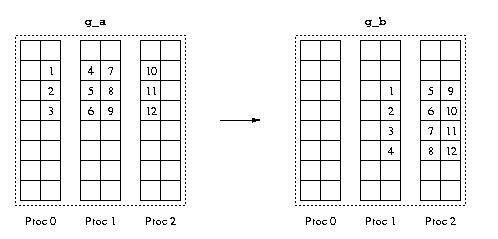
\includegraphics[width=10cm]{copy1}\tabularnewline
\hline
\end{tabular}

One step further, if one also want to perform the transpose operation
during the copying, i.e. set \texttt{\textcolor{black}{trans = 1}},
it will look like: 

\begin{tabular}{|c|}
\hline 
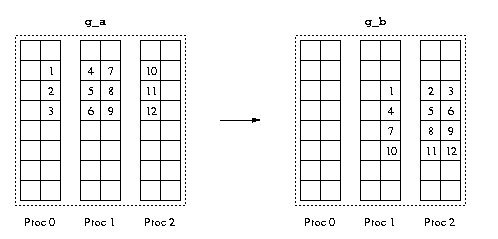
\includegraphics[width=10cm]{copy2}\tabularnewline
\hline
\end{tabular}

If there is no reshaping or transpose, the operation can be fast (internally
calling \texttt{nga\_put}). Otherwise, it would be slow (internally
calling \texttt{nga\_scatter}, where extra time is spent on preparing
the indices). Also note that extra memory is required to hold the
indices if the operation involves reshaping or transpose. 


\section{Linear Algebra }

Global arrays provide three linear algebra operations: addition, multiplication,
and dot product. There are two sets of functions, one for the whole
array and the other for the patches. 


\subsection{Whole Arrays }

The function
\begin{verbatim}
\textcolor{blue}{Fortran}~subroutine~\href{http://www.emsl.pnl.gov/docs/global/ga_ops.html\#ga_add}{ga\_{}add}(alpha,~g\_a,~beta,~g\_b,~g\_c)~

\textcolor{blue}{C}~~~~~~~void~\href{http://www.emsl.pnl.gov/docs/global/c_nga_ops.html\#ga_add}{GA\_{}Add}(void~{*}alpha,~int~g\_a,~

~~~~~~~~void~{*}beta,int~g\_b,~int~g\_c)~

\textcolor{blue}{C++}~void~GA::GlobalArray::add(void~{*}alpha,~~

~~~~~~~~const~GA::GlobalArray{*}~g\_a,~

~~~~~~~~void~{*}beta,~const~GA::GlobalArray{*}~g\_b)
\end{verbatim}
adds two arrays, \texttt{g\_a} and \texttt{g\_b}, and saves the results
to \texttt{g\_c}. The two source arrays can be scaled by certain factors.
This operation requires the two source arrays have the same number
of elements and the same data types, but the arrays can have different
shapes or distributions.\texttt{ g\_c} can also be \texttt{g\_a} or
\texttt{g\_b}. It is encouraged to use this function when the two
source arrays are identical in distributions and shapes, because of
its efficiency. It would be less efficient if the two source arrays
are different in distributions or shapes.

Matrix multiplication operates on two matrices, therefore the array
must be two dimensional. The function
\begin{verbatim}
\textcolor{blue}{Fortran}~subroutine~\href{http://www.emsl.pnl.gov/docs/global/ga_ops.html\#ga_dgemm}{ga\_{}dgemm}(transa,~transb,~m,~n,~k,~

~~~~~~~~~~~~~~alpha,~g\_a,~g\_b,~beta,~g\_c~)~

\textcolor{blue}{C}~~~~~~~void~\href{http://www.emsl.pnl.gov/docs/global/c_nga_ops.html\#ga_dgemm}{GA\_{}Dgemm}(char~ta,~char~tb,~int~m,~int~n,~

~~~~~~~~~~~~~~int~k,~double~alpha,~int~g\_a,~int~g\_b,~

~~~~~~~~~~~~~~double~beta,~int~g\_c~)~

\textcolor{blue}{C++}~~~~~void~GA::GlobalArray::dgemm(char~ta,~char~tb,~

~~~~~~~~~~~~~~int~m,~int~n,~int~k,~double~alpha,~

~~~~~~~~~~~~~~const~GA::GlobalArray{*}~g\_a,~const~GA::GlobalArray{*}~

~~~~~~~~~~~~~~g\_b,~double~beta)
\end{verbatim}
Performs one of the matrix-matrix operations:

\emph{C := alpha{*}op( A ){*}op( B ) + beta{*}C,}

where op( X ) is one of

\emph{op( X ) = X or op( X ) = X',}

alpha and beta are scalars, and \emph{A}, \emph{B,} and \emph{C} are
matrices, with \emph{op( A ) }an \emph{m} by \emph{k} matrix, \emph{op(
B )} a \emph{k} by \emph{n} matrix and \emph{C} an \emph{m} by \emph{n}
matrix.

On entry, transa specifies the form of \emph{op( A )} to be used in
the matrix multiplication as follows: 

\emph{ta = 'N'} or\emph{ 'n', op( A ) = A}. 

\emph{ta = 'T'} or \emph{'t', op( A ) = A'}.

The function
\begin{verbatim}
Fortran~integer~function~ga\_idot(g\_a,~g\_b)~

~~~~~~~~double~precision~function~\href{http://www.emsl.pnl.gov/docs/global/ga_ops.html\#ga_ddot}{ga\_{}ddot}(g\_a,~g\_b)

~~~~~~~~double~complex~function~\href{http://www.emsl.pnl.gov/docs/global/ga_ops.html\#ga_zdot}{ga\_{}zdot}(g\_a,~g\_b)~

C~~~~~~~long~\href{http://www.emsl.pnl.gov/docs/global/c_nga_ops.html\#ga_dot}{GA\_{}Idot}(int~g\_a,~int~g\_b)~

~~~~~~~~double~G\href{http://www.emsl.pnl.gov/docs/global/c_nga_ops.html\#ga_dot}{GA\_{}Ddot}A\_Ddot(int~g\_a,~int~g\_b)~

~~~~~~~~DoubleComplex~\href{http://www.emsl.pnl.gov/docs/global/c_nga_ops.html\#ga_dot}{GA\_{}Zdot}GA\_Zdot(int~g\_a,~int~g\_b)~

C++~~~~~long~GA::GlobalArray::idot

~~~~~~~~~~~~~~~~~(const~GA::GlobalArray{*}~g\_a)~

~~~~~~~~double~GA::GlobalArray::ddot

~~~~~~~~~~~~~~~~~(const~GA::GlobalArray{*}~g\_a)~

~~~~~~~~DoubleComplex~GA::GlobalArray::zdot

~~~~~~~~~~~~~~~~~(const~GA::GlobalArray{*}~g\_a)
\end{verbatim}
computes the element-wise dot product of two arrays. It is available
as three separate functions, corresponding to \emph{integer}, \emph{double
precision} and \emph{double complex} data types.

The following functions apply to the 2-dimensional whole arrays only.
There are no corresponding functions for patch operations.

The function
\begin{verbatim}
\textcolor{blue}{Fortran}~subroutine~\href{http://www.emsl.pnl.gov/docs/global/ga_ops.html\#ga_symmetrize}{ga\_{}symmetrize}(g\_a)~

\textcolor{blue}{C}~~~~~~~void~\href{http://www.emsl.pnl.gov/docs/global/c_nga_ops.html\#ga_symmetrize}{GA\_{}Symmetrize}(int~g\_a)~

\textcolor{blue}{C++}~~~~~void~GA::GlobalArray::symmetrize()
\end{verbatim}
symmetrizes matrix A represented with handle \texttt{g\_a}:\emph{A
= .5 {*} (A+A')}.

The function
\begin{verbatim}
\textcolor{blue}{Fortran}~subroutine~\href{http://www.emsl.pnl.gov/docs/global/ga_ops.html\#ga_transpose}{ga\_{}transpose}(g\_a,~g\_b)~

\textcolor{blue}{C}~~~~~~~void~\href{http://www.emsl.pnl.gov/docs/global/c_nga_ops.html\#ga_transpose}{GA\_{}Transpose}(int~g\_a,~int~g\_b)~

\textcolor{blue}{C++}~~~~~void~GA::GlobalArray::transpose

~~~~~~~~~~~~~(const~GA::GlobalArray{*}~g\_a)
\end{verbatim}
transposes a matrix: B = A'.


\subsection{Patches }

The functions
\begin{verbatim}
\textcolor{green}{n-D}\textcolor{blue}{Fortran}~subroutine~\href{http://www.emsl.pnl.gov/docs/global/ga_ops.html\#ga_add_patch}{nga\_{}add\_{}patch}(alpha,~g\_a,~

~~~~~~~~~~~~~~~~~~~~~~alo,~ahi,~beta,~g\_b,~blo,~

~~~~~~~~~~~~~~~~~~~~~~bhi,~g\_c,~clo,~chi)~

\textcolor{green}{2-D}\textcolor{blue}{Fortran}~subroutine~\href{http://www.emsl.pnl.gov/docs/global/ga_ops.html\#ga_add_patch}{ga\_{}add\_{}patch}(alpha,~g\_a,~

~~~~~~~~~~~~~~~~~~~~~~ailo,~aihi,~ajlo,~ajhi,~

~~~~~~~~~~~~~~~~~~~~~~beta,~g\_b,~bilo,~bihi,~bjlo,~

~~~~~~~~~~~~~~~~~~~~~~bjhi,~g\_c,~cilo,~cihi,~cjlo,~cjhi)~

\textcolor{blue}{C}~~~~~~~~~~void~\href{http://www.emsl.pnl.gov/docs/global/c_nga_ops.html\#ga_add_patch}{NGA\_{}Add\_{}patch}(void~{*}alpha,~int~g\_a,~int~

~~~~~~~~~~~~~~~~~~~~~~alo{[}{]},~int~ahi{[}{]},~void~{*}beta,~

~~~~~~~~~~~~~~~~~~~~~~int~g\_b,~int~blo{[}{]},~int~bhi{[}{]},~

~~~~~~~~~~~~~~~~~~~~~~int~g\_c,~int~clo{[}{]},~int~chi{[}{]})~

\textcolor{blue}{C++}~~~~~~~~void~GA::GlobalArray::addPatch(void~{*}alpha,~

~~~~~~~~~~~~~~~~~~~~~~const~GA::GlobalArray{*}~g\_a,~

~~~~~~~~~~~~~~~~~~~~~~int~alo{[}{]},~int~ahi{[}{]},~void~{*}beta,~

~~~~~~~~~~~~~~~~~~~~~~const~GA::GlobalArray{*}~g\_b,~int~blo{[}{]},~

~~~~~~~~~~~~~~~~~~~~~~int~bhi{[}{]},~int~clo{[}{]},~int~chi{[}{]})~
\end{verbatim}
add element-wise two patches and save the results into another patch.
Even though it supports the addition of two patches with different
distributions or different shapes (the number of elements must be
the same), the operation can be expensive, because there can be extra
copies which effect memory consumption. The two source patches can
be scaled by a factor for the addition. The function is smart enough
to detect the case that the patches are exactly the same but the global
arrays are different in shapes. It handles the case as if for the
arrays were identically distributed, thus the performance will not
suffer.

The matrix multiplication is the only operation on array patches that
is restricted to the two dimensional domain, because of its nature.
It works for\emph{ double} and \emph{double complex} data types. The
prototype is
\begin{verbatim}
\textcolor{blue}{Fortran}~subroutine~\href{http://www.emsl.pnl.gov/docs/global/ga_ops.html\#ga_matmul_patch}{ga\_{}matmul\_{}patch}(transa,~transb,~

~~~~~~~~~~~~~~~~~~~alpha,~beta,~g\_a,~ailo,~aihi,~

~~~~~~~~~~~~~~~~~~~ajlo,~ajhi,~g\_b,~bilo,~bihi,~bjlo,~

~~~~~~~~~~~~~~~~~~~bjhi,~g\_c,~cilo,~cihi,~cjlo,~cjhi)~

\textcolor{blue}{C}~~~~~~~void~\href{http://www.emsl.pnl.gov/docs/global/c_nga_ops.html\#ga_matmul_patch}{GA\_{}Matmul\_{}patch}(char~{*}transa,~char{*}~transb,

~~~~~~~~~~~~~~~~~~~void{*}~alpha,~void~{*}beta,~int~g\_a,~

~~~~~~~~~~~~~~~~~~~int~ailo,~int~aihi,~int~ajlo,~int~ajhi,~

~~~~~~~~~~~~~~~~~~~int~g\_b,~int~bilo,~int~bihi,~int~bjlo,~

~~~~~~~~~~~~~~~~~~~int~bjhi,~int~g\_c,~int~cilo,~int~cihi,~

~~~~~~~~~~~~~~~~~~~int~cjlo,~int~cjhi)~

\textcolor{blue}{C++}~~~~~void~GA::GlobalArray::matmulPatch(char~{*}transa,

~~~~~~~~~~~~~~~~~~~char{*}~transb,~void{*}~alpha,~void~{*}beta,~

~~~~~~~~~~~~~~~~~~~const~GlobalArray~{*}~g\_a,~int~ailo,~

~~~~~~~~~~~~~~~~~~~int~aihi,~int~ajlo,~int~ajhi,~const~

~~~~~~~~~~~~~~~~~~~GlobalArray~{*}~g\_b,~int~bilo,~int~bihi,~

~~~~~~~~~~~~~~~~~~~int~bjlo,~int~bjhi,~int~cilo,~int~cihi,~

~~~~~~~~~~~~~~~~~~~int~cjlo,~int~cjhi)
\end{verbatim}
It performs
\begin{verbatim}
C{[}cilo:cihi,cjlo:cjhi{]}~:=~alpha{*}~AA{[}ailo:aihi,ajlo:ajhi{]}~{*}

~~~~~BB{[}bilo:bihi,bjlo:bjhi{]}~)~+~beta{*}C{[}cilo:cihi,cjlo:cjhi{]}
\end{verbatim}
where \emph{AA = op(A), BB = op(B),} and \emph{op( X )} is one of

\emph{op( X ) = X or op( X ) = X',}

Valid values for transpose argument:\emph{ 'n', 'N', 't', 'T'}.

The dot operation computes the element-wise dot product of two (possibly
transposed) patches. It is implemented as three separate functions,
corresponding to integer, double precision and double complex data
types. They are
\begin{verbatim}
\textcolor{green}{n-D}\textcolor{blue}{Fortran}~integer~function~nga\_idot\_patch(g\_a,~ta,~

~~~~~~~~~~~~~~~~~alo,~ahi,~g\_b,~tb,~blo,~bhi)~

~~~~~~~~~~~double~precision~functionn~\href{http://www.emsl.pnl.gov/docs/global/ga_ops.html\#ga_ddot_patch}{ga\_{}ddot\_{}patch}

~~~~~~~~~~~~~~~~~(g\_a,~ta,~alo,~ahi,~g\_b,~tb,~blo,~bhi)~

~~~~~~~~~~~double~complex~functionn~\href{http://www.emsl.pnl.gov/docs/global/ga_ops.html\#ga_zdot_patch}{ga\_{}zdot\_{}patch}

~~~~~~~~~~~~~~~~~(g\_a,~ta,~alo,~ahi,~g\_b,~tb,~blo,~bhi)



\textcolor{green}{2-D}\textcolor{blue}{Fortran}~integer~function~ga\_idot\_patch(g\_a,~ta,~ailo,~aihi,

~~~~~~~~~~~~~~~~~ajlo,~ailo,~g\_b,~tb,~bilo,~bihi,~bjlo,~bjhi)~

~~~~~~~~~~~double~precision~function~\href{http://www.emsl.pnl.gov/docs/global/ga_ops.html\#ga_ddot_patch}{ga\_{}ddot\_{}patch}(g\_a,~ta,~

~~~~~~~~~~~~~~~~~ailo,~aihi,~ajlo,~ailo,~g\_b,~tb,~bilo,~bihi,~

~~~~~~~~~~~~~~~~~bjlo,~bjhi)~

~~~~~~~~~~~double~complex~function~\href{http://www.emsl.pnl.gov/docs/global/ga_ops.html\#ga_zdot_patch}{ga\_{}zdot\_{}patch}(g\_a,~ta,~ailo,~

~~~~~~~~~~~~~~~~~aihi,~ajlo,~ailo,~g\_b,~tb,~bilo,~bihi,~bjlo,~bjhi)



\textcolor{blue}{C}~~~~~~~~~~Integer~\href{http://www.emsl.pnl.gov/docs/global/c_nga_ops.html\#ga_dot_patch}{NGA\_{}Idot\_{}patch}(int~g\_a,~char{*}~ta,~int~alo{[}{]},~

~~~~~~~~~~~~~~~~~int~ahi{[}{]},~int~g\_b,~char{*}~tb,~int~blo{[}{]},~

~~~~~~~~~~~~~~~~~int~bhi{[}{]})~

~~~~~~~~~~~double~\href{http://www.emsl.pnl.gov/docs/global/c_nga_ops.html\#ga_dot_patch}{NGA\_{}Ddot\_{}patch}(int~g\_a,~char{*}~ta,~int~alo{[}{]},~

~~~~~~~~~~~~~~~~~int~ahi{[}{]},~int~g\_b,~char{*}~tb,~int~blo{[}{]},~

~~~~~~~~~~~~~~~~~int~bhi{[}{]})~

~~~~~~~~~~~DoubleComplex~\href{http://www.emsl.pnl.gov/docs/global/c_nga_ops.html\#ga_dot_patch}{NGA\_{}Zdot\_{}patch}(int~g\_a,~char{*}~ta,~

~~~~~~~~~~~~~~~~~int~alo{[}{]},~int~ahi{[}{]},~int~g\_b,~char{*}~tb,~

~~~~~~~~~~~~~~~~~int~blo{[}{]},~int~bhi{[}{]})



\textcolor{blue}{C++~}~~~~~~~IntegerGA::GlobalArray::idotPatch(const~GA::GlobalArray{*}

~~~~~~~~~~~~~~~~~g\_a,~char{*}~ta,~int~alo{[}{]},~int~ahi{[}{]},~char{*}~

~~~~~~~~~~~~~~~~~tb,~int~blo{[}{]},~int~bhi{[}{]})~

~~~~~~~~~~~double~GA::GlobalArray::ddotPatch(const~GA::GlobalArray{*}

~~~~~~~~~~~~~~~~~g\_a,~char{*}~ta,~int~alo{[}{]},~int~ahi{[}{]},~char{*}~tb,~

~~~~~~~~~~~~~~~~~int~blo{[}{]},~int~bhi{[}{]})~

~~~~~~~~~~~DoubleComplex~GA::GlobalArray::zdotPatch

~~~~~~~~~~~~~~~~~(const~GA::GlobalArray{*}~g\_a,~char{*}~ta,~int~alo{[}{]},~

~~~~~~~~~~~~~~~~~int~ahi{[}{]},~char{*}~tb,~int~blo{[}{]},~int~bhi{[}{]})
\end{verbatim}
The patches should be of the same data types and have the same number
of elements. Like the array addition, if the source patches have different
distributions/shapes, or it requires transpose, the operation would
be less efficient, because there could be extra copies and/or memory
consumption. 


\subsection{Element-wise operations }

These operations work on individual array elements rather than arrays
as matrices in the sense of linear algebra operations. For example
multiplication of elements stored in arrays is a completely different
operation than matrix multiplication.
\begin{verbatim}
\textcolor{blue}{Fortran}~subroutine~\href{http://www.emsl.pnl.gov/docs/global/ga_ops.html\#ga_abs_value}{ga\_{}abs\_{}value}(g\_a)~

\textcolor{blue}{C}~~~~~~void~\href{http://www.emsl.pnl.gov/docs/global/c_nga_ops.html\#ga_abs_value}{GA\_{}Abs\_{}value}(int~g\_a)

\textcolor{blue}{C++}~~~~void~GA::GlobalArray::absValue(int~g\_a)
\end{verbatim}
Take element-wise absolute value of the array. 
\begin{verbatim}
\textcolor{blue}{Fortran}~subroutine~\href{http://www.emsl.pnl.gov/docs/global/ga_ops.html\#ga_abs_value_patch}{ga\_{}abs\_{}value\_{}patch}(g\_a,~lo,~hi)~

\textcolor{blue}{C}~~~~~~~void~\href{http://www.emsl.pnl.gov/docs/global/c_nga_ops.html\#ga_abs_value_patch}{GA\_{}Abs\_{}value\_{}patch}(int~g\_a,~int~lo{[}{]},~int~hi{[}{]})~

\textcolor{blue}{C++}~~~~~void~GA::GlobalArray::absValuePatch

~~~~~~~~~~~~~(int~lo{[}{]},~int~hi{[}{]})
\end{verbatim}
Take element-wise absolute value of the patch.
\begin{verbatim}
\textcolor{blue}{Fortran}~subroutine~\href{http://www.emsl.pnl.gov/docs/global/ga_ops.html\#ga_add_constant}{ga\_{}add\_{}constant}(g\_a,~alpha)~

\textcolor{blue}{C}~~~~~~~void~\href{http://www.emsl.pnl.gov/docs/global/c_nga_ops.html\#ga_add_constant}{GA\_{}Add\_{}constant}(int~g\_a,~void{*}~alpha)~

\textcolor{blue}{C++}~~~~~void~GA::GlobalArray::addConstant(void{*}~alpha)
\end{verbatim}
Add the contant pointed by alpha to each element of the array. 
\begin{verbatim}
\textcolor{blue}{Fortran}~subroutine~\href{http://www.emsl.pnl.gov/docs/global/ga_ops.html\#ga_add_constant_patch}{ga\_{}add\_{}constant\_{}patch}(g\_a,~lo,~hi,~alpha)~

\textcolor{blue}{C}~~~~~~~void~\href{http://www.emsl.pnl.gov/docs/global/c_nga_ops.html\#ga_add_constant_patch}{GA\_{}Add\_{}constant\_{}patch}(int~g\_a,~int~lo{[}{]},~

~~~~~~~~~~~~~int~hi{[}{]},~void{*}alpha)~

\textcolor{blue}{C++}~~~~~void~GA::GlobalArray::addConstantPatch(void{*}~alpha)
\end{verbatim}
Add the contant pointed by alpha to each element of the patch. 
\begin{verbatim}
\textcolor{blue}{Fortran~}subroutine~\href{http://www.emsl.pnl.gov/docs/global/ga_ops.html\#ga_recip}{ga\_{}recip}(g\_a)

\textcolor{blue}{C}~~~~~~~void~\href{http://www.emsl.pnl.gov/docs/global/c_nga_ops.html\#ga_recip}{GA\_{}Recip}(int~g\_a)

\textcolor{blue}{C++}~~~~~void~GA::GlobalArray::recip()
\end{verbatim}
Take element-wise reciprocal of the array.
\begin{verbatim}
\textcolor{blue}{Fortran}~subroutine~\href{http://www.emsl.pnl.gov/docs/global/ga_ops.html\#ga_recip_patch}{ga\_{}recip\_{}patch}(g\_a,~lo,~hi)~

\textcolor{blue}{C}~~~~~~~void~\href{http://www.emsl.pnl.gov/docs/global/c_nga_ops.html\#ga_recip_patch}{GA\_{}Recip\_{}patch}(int~g\_a,~int~lo{[}{]},~int~hi{[}{]})

\textcolor{blue}{C++~}~~~~void~GA::GlobalArray::recipPatch(int~lo{[}{]},~int~hi{[}{]})
\end{verbatim}
Take element-wise reciprocal of the patch.
\begin{verbatim}
\textcolor{blue}{Fortran}~subroutine~\href{http://www.emsl.pnl.gov/docs/global/ga_ops.html\#ga_elem_multiply}{ga\_{}elem\_{}multiply}(g\_a,~g\_b,~g\_c)

\textcolor{blue}{C}~~~~~~~void~\href{http://www.emsl.pnl.gov/docs/global/c_nga_ops.html\#ga_elem_multiply}{GA\_{}Elem\_{}multiply}(int~g\_a,~int~g\_b,~int~g\_c)~

\textcolor{blue}{C++}~~~~~void~GA::GlobalArray::elemMultiply(const~

~~~~~~~~~~~~~~~~~GA::GlobalArray~{*}~g\_a,~

~~~~~~~~~~~~~~~~~const~GA::GlobalArray~{*}~g\_b)
\end{verbatim}
Computes the element-wise product of the two arrays which must be
of the same types and same number of elements. For two-dimensional
arrays,

c(i, j) = a(i,j){*}b(i,j)

The result (c) may replace one of the input arrays (a/b). 
\begin{verbatim}
\textcolor{blue}{Fortra}n~subroutine~\href{http://www.emsl.pnl.gov/docs/global/ga_ops.html\#ga_elem_multiply_patch}{ga\_{}elem\_{}multiply\_{}\_{}patch}(g\_a,~alo,~

~~~~~~~~~~~~~~~ahi,~g\_b,~blo,~bhi,~g\_c,~clo,chi)~

\textcolor{blue}{C}~~~~~~~void~\href{http://www.emsl.pnl.gov/docs/global/c_nga_ops.html\#ga_elem_multiply_patch}{GA\_{}Elem\_{}multiply\_{}\_{}patch}(int~g\_a,~int~alo{[}{]},~

~~~~~~~~~~~~~~~int~ahi{[}{]},~int~g\_b,~int~blo{[}{]},~int~bhi{[}{]},

~~~~~~~~~~~~~~~int~g\_c,~int~clo{[}{]},~int~chi{[}{]})~

\textcolor{blue}{C++~}~~~~void~GA::GlobalArray::elemMultiplyPatch

~~~~~~~~~~~~~~~(~const~GA::GlobalArray~{*}~g\_a,~int~alo{[}{]},~

~~~~~~~~~~~~~~~int~ahi{[}{]},~const~GA::GlobalArray~{*}~g\_b,~

~~~~~~~~~~~~~~~int~blo{[}{]},~int~bhi{[}{]},~int~clo{[}{]},~int~chi{[}{]})
\end{verbatim}
Computes the element-wise product of the two patches which must be
of the same types and same number of elements. For two-dimensional
arrays,

c(i, j) = a(i,j){*}b(i,j)

The result (c) may replace one of the input arrays (a/b).
\begin{verbatim}
\textcolor{blue}{Fortran}~subroutine~\href{http://www.emsl.pnl.gov/docs/global/ga_ops.html\#ga_elem_divide}{ga\_{}elem\_{}divide}(g\_a,~g\_b,~g\_c)~

\textcolor{blue}{C}~~~~~~~void~\href{http://www.emsl.pnl.gov/docs/global/c_nga_ops.html\#ga_elem_divide}{GA\_{}Elem\_{}divide}(Integer~g\_a,~Integer~

~~~~~~~~~~~~~~~~~~~~~~~g\_b,~Integer~g\_c)

\textcolor{blue}{C++}~~~~~void~GA::GlobalArray::elemDivide(const~GA::GlobalArray~{*}~

~~~~~~~~~~~~~~~~~~~~~~~g\_a,~const~GA::GlobalArray~{*}~g\_b)
\end{verbatim}
Computes the element-wise quotient of the two arrays which must be
of the same types and same number of elements. For two-dimensional
arrays,

c(i, j) = a(i,j)/b(i,j)

The result (c) may replace one of the input arrays (a/b). If one of
the elements of array g\_b is zero, the quotient for the element of
g\_c will be set to GA\_NEGATIVE\_INFINITY. 
\begin{verbatim}
\textcolor{blue}{Fortran}~subroutine~\href{http://www.emsl.pnl.gov/docs/global/ga_ops.html\#ga_elem_divide_patch}{ga\_{}elem\_{}divide\_{}\_{}patch}(g\_a,~alo,~

~~~~~~~~~~~~~~~~~~~ahi,~g\_b,~blo,~bhi,~g\_c,~clo,~chi)~

\textcolor{blue}{C}~~~~~~~void~\href{http://www.emsl.pnl.gov/docs/global/c_nga_ops.html\#ga_elem_divide_patch}{GA\_{}Elem\_{}divide\_{}\_{}patch}(int~g\_a,~int~alo{[}{]},

~~~~~~~~~~~~~~~~~~~int~ahi{[}{]},~int~g\_b,~int~blo{[}{]},~int~bhi{[}{]},~

~~~~~~~~~~~~~~~~~~~int~g\_c,~int~clo{[}{]},~int~chi{[}{]})~

\textcolor{blue}{C++}~~~~~void~GA::GlobalArray::elemDividePatch(~const~

~~~~~~~~~~~~~~~~~~~GA::GlobalArray~{*}~g\_a,~int~alo{[}{]},~

~~~~~~~~~~~~~~~~~~~int~ahi{[}{]},~const~GA::GlobalArray~{*}~g\_b,~

~~~~~~~~~~~~~~~~~~~int~blo{[}{]},~int~bhi{[}{]},~int~clo{[}{]},~int~chi{[}{]})
\end{verbatim}
Computes the element-wise quotient of the two patches which must be
of the same types and same number of elements. For two-dimensional
arrays,

c(i, j) = a(i,j)/b(i,j)

The result (c) may replace one of the input arrays (a/b). 
\begin{verbatim}
\textcolor{blue}{Fortran}~subroutine~\href{http://www.emsl.pnl.gov/docs/global/ga_ops.html\#ga_elem_maximum}{ga\_{}elem\_{}maximum}(g\_a,~g\_b,~g\_c)~

\textcolor{blue}{C}~~~~~~~void~\href{http://www.emsl.pnl.gov/docs/global/c_nga_ops.html\#ga_elem_maximum}{GA\_{}Elem\_{}maximum}(Integer~g\_a,~Integer~g\_b,~

~~~~~~~~~~~~~~~~~~~Integer~g\_c)

\textcolor{blue}{C++}~~~~~void~GA::GlobalArray::elemMaximum(const~GA::GlobalArray~

~~~~~~~~~~~~~~~~~~~{*}~g\_a,~const~GA::GlobalArray~{*}~g\_b)
\end{verbatim}
Computes the element-wise maximum of the two arrays which must be
of the same types and same number of elements. For two dimensional
arrays,

c(i, j) = max\{a(i,j), b(i,j)\}

The result (c) may replace one of the input arrays (a/b). 
\begin{verbatim}
\textcolor{blue}{Fortran}~subroutine~\href{http://www.emsl.pnl.gov/docs/global/ga_ops.html\#ga_elem_maximum_patch}{ga\_{}elem\_{}maximum\_{}\_{}patch}(g\_a,~alo,

~~~~~~~~~~~~~~~~~~~ahi,~g\_b,~blo,~bhi,~g\_c,~clo,~chi)~

\textcolor{blue}{C}~~~~~~~void~\href{http://www.emsl.pnl.gov/docs/global/c_nga_ops.html\#ga_elem_maximum_patch}{GA\_{}Elem\_{}maximum\_{}\_{}patch}(int~g\_a,~int~alo{[}{]},

~~~~~~~~~~~~~~~~~~~int~ahi{[}{]},~int~g\_b,~int~blo{[}{]},~int~bhi{[}{]},~

~~~~~~~~~~~~~~~~~~~int~g\_c,~int~clo{[}{]},~int~chi{[}{]})

\textcolor{blue}{C++}~~~~~void~GA::GlobalArray::elemMaximumPatch(const~

~~~~~~~~~~~~~~~~~~~GA::GlobalArray~{*}~g\_a,~int~alo{[}{]},~int~ahi{[}{]},~

~~~~~~~~~~~~~~~~~~~const~GA::GlobalArray~{*}~g\_b,~int~blo{[}{]},~

~~~~~~~~~~~~~~~~~~~int~bhi{[}{]},~int~clo{[}{]},~int~chi{[}{]})
\end{verbatim}
Computes the element-wise maximum of the two patches which must be
of the same types and same number of elements. For two-dimensional
of noncomplex arrays,

c(i, j) = max\{a(i,j), b(i,j)\}

If the data type is complex, then c(i, j).real = max\{ |a(i,j)|, |b(i,j)|\}
while c(i,j).image = 0.

The result (c) may replace one of the input arrays (a/b). 
\begin{verbatim}
\textcolor{blue}{Fortran}~subroutine~\href{http://www.emsl.pnl.gov/docs/global/ga_ops.html\#ga_elem_minimum}{ga\_{}elem\_{}minimum}(g\_a,~g\_b,~g\_c)~

\textcolor{blue}{C}~~~~~~~void~\href{http://www.emsl.pnl.gov/docs/global/c_nga_ops.html\#ga_elem_minimum}{GA\_{}Elem\_{}minimum}(Integer~g\_a,~Integer~g\_b,~Integer~g\_c);

\textcolor{blue}{C++~}~~~~void~GA::GlobalArray::elemMinimum(const~GA::GlobalArray~{*}

~~~~~~~~~~~~~~~~~g\_a,~const~GA::GlobalArray~{*}~g\_b)
\end{verbatim}
Computes the element-wise minimum of the two arrays which must be
of the same types and same number of elements. For two dimensional
arrays,

c(i, j) = min\{a(i,j), b(i,j)\}

The result (c) may replace one of the input arrays (a/b). 
\begin{verbatim}
\textcolor{blue}{Fortran}~subroutine~\href{http://www.emsl.pnl.gov/docs/global/ga_ops.html\#ga_elem_minimum_patch}{ga\_{}elem\_{}minimum\_{}\_{}patch}(g\_a,~alo,~ahi,

~~~~~~~~~~~~~~~~~~~g\_b,~blo,~bhi,~g\_c,~clo,~chi)~

\textcolor{blue}{C}~~~~~~~void~\href{http://www.emsl.pnl.gov/docs/global/c_nga_ops.html\#ga_elem_minimum_patch}{GA\_{}Elem\_{}minimum\_{}\_{}patch}(int~g\_a,~int~alo{[}{]},~

~~~~~~~~~~~~~~~~~~~int~ahi{[}{]},~int~g\_b,~int~blo{[}{]},~int~bhi{[}{]},~

~~~~~~~~~~~~~~~~~~~int~g\_c,~int~clo{[}{]},~int~chi{[}{]})

\textcolor{blue}{C++}~~~~~void~GA::GlobalArray::elemMinimumPatch~~

~~~~~~~~~~~~~~~~~~~(const~GA::GlobalArray~{*}~g\_a,~int~alo{[}{]},~

~~~~~~~~~~~~~~~~~~~int~ahi{[}{]},~const~GA::GlobalArray~{*}~g\_b,~

~~~~~~~~~~~~~~~~~~~int~blo{[}{]},~int~bhi{[}{]},~int~clo{[}{]},~int~chi{[}{]})
\end{verbatim}
Computes the element-wise minimum of the two patches which must be
of the same types and same number of elements. For two-dimensional
of noncomplex arrays,

c(i, j) = min\{a(i,j), b(i,j)\}

If the data type is complex, then

c(i, j).real = min\{ |a(i,j)|, |b(i,j)|\} while c(i,j).image = 0.

The result (c) may replace one of the input arrays (a/b). 
\begin{verbatim}
\textcolor{blue}{Fortran}~subroutine~\href{http://www.emsl.pnl.gov/docs/global/ga_ops.html\#ga_shift_diagonal}{ga\_{}shift\_{}diagonal}(g\_a,~c)~

\textcolor{blue}{C}~~~~~~~void~\href{http://www.emsl.pnl.gov/docs/global/c_nga_ops.html\#ga_shift_diagonal}{GA\_{}Shift\_{}diagonal}(int~g\_a,~void~{*}c)~

\textcolor{blue}{C++}~~~~~void~GA::GlobalArray::shiftDiagonal(void~{*}c)
\end{verbatim}
Adds this constant to the diagonal elements of the matrix.
\begin{verbatim}
\textcolor{blue}{Fortran}~subroutine~\href{http://www.emsl.pnl.gov/docs/global/ga_ops.html\#ga_set_diagonal}{ga\_{}set\_{}diagonal}(g\_a,~g\_v)~

\textcolor{blue}{C}~~~~~~~void~\href{http://www.emsl.pnl.gov/docs/global/c_nga_ops.html\#ga_set_diagonal}{GA\_{}Set\_{}diagonal}(int~g\_a,~int~g\_v)

\textcolor{blue}{C++}~~~~~void~GA::GlobalArray::setDiagonal~

~~~~~~~~~~~~~(const~GA::GlobalArray~{*}~g\_v)
\end{verbatim}
Sets the diagonal elements of this matrix g\_a with the elements of
the vector g\_v.
\begin{verbatim}
Fortran~subroutine~\href{http://www.emsl.pnl.gov/docs/global/ga_ops.html\#ga_zero_diagonal}{ga\_{}zero\_{}diagonal}(~g\_a)~

C~~~~~~~void~\href{http://www.emsl.pnl.gov/docs/global/c_nga_ops.html\#ga_zero_diagonal}{GA\_{}Zero\_{}diagonal}(int~g\_a)~

C++~~~~~void~GA::GlobalArray::zeroDiagonal()
\end{verbatim}
Sets the diagonal elements of this matrix g\_a with zeros. 
\begin{verbatim}
\textcolor{blue}{Fortran}~subroutine~\href{http://www.emsl.pnl.gov/docs/global/ga_ops.html\#ga_add_diagonal}{ga\_{}add\_{}diagonal}(g\_a,~g\_v)~

\textcolor{blue}{C}~~~~~~~void~\href{http://www.emsl.pnl.gov/docs/global/c_nga_ops.html\#ga_add_diagonal}{GA\_{}Add\_{}diagonal}(int~g\_a,~int~g\_v)

\textcolor{blue}{C++}~~~~~void~GA::GlobalArray::addDiagonal(const~

~~~~~~~~~~~~~~~~~~~~GA::GlobalArray~{*}~g\_v)
\end{verbatim}
Adds the elements of the vector g\_v to the diagonal of this matrix
g\_a. 
\begin{verbatim}
\textcolor{blue}{Fortran}~subroutine~\href{http://www.emsl.pnl.gov/docs/global/ga_ops.html\#ga_get_diag}{ga\_{}get\_{}diag}(g\_a,~g\_v)~

\textcolor{blue}{C}~~~~~~~void~\href{http://www.emsl.pnl.gov/docs/global/c_nga_ops.html\#ga_get_diag}{GA\_{}Get\_{}diag}(int~g\_a,~int~g\_v)

\textcolor{blue}{C++~}~~~~void~GA::GlobalArray::getDiagonal

~~~~~~~~~~~~~~~~~~~~(const~GA::GlobalArray~{*}~g\_v)
\end{verbatim}
Inserts the diagonal elements of this matrix g\_a into the vector
g\_v. 
\begin{verbatim}
\textcolor{blue}{Fortran}~subroutine~\href{http://www.emsl.pnl.gov/docs/global/ga_ops.html\#ga_scale_rows}{ga\_{}scale\_{}rows}(~g\_a,~g\_v)

\textcolor{blue}{C}~~~~~~~void~\href{http://www.emsl.pnl.gov/docs/global/c_nga_ops.html\#ga_scale_rows}{GA\_{}Scale\_{}rows}(int~g\_a,~int~g\_v)~

\textcolor{blue}{C++}~~~~~void~GA::GlobalArray::scaleRows

~~~~~~~~~~~~~~~~~~~~(const~GA::GlobalArray~{*}~g\_v)
\end{verbatim}
Scales the rows of this matrix g\_a using the vector g\_v. 
\begin{verbatim}
\textcolor{blue}{Fortran}~subroutine~\href{http://www.emsl.pnl.gov/docs/global/ga_ops.html\#ga_scale_cols}{ga\_{}scale\_{}cols}(g\_a,~g\_v)~

\textcolor{blue}{C}~~~~~~~void~\href{http://www.emsl.pnl.gov/docs/global/c_nga_ops.html\#ga_scale_cols}{GA\_{}Scale\_{}cols}(int~g\_a,~int~g\_v)~

\textcolor{blue}{C++}~~~~~void~GA::GlobalArray::scaleCols

~~~~~~~~~~~~~~~~~~~~(const~GA::GlobalArray~{*}~g\_v)
\end{verbatim}
Scales the columns of this matrix g\_a using the vector g\_v. 
\begin{verbatim}
\textcolor{blue}{Fortran}~subroutine~\href{http://www.emsl.pnl.gov/docs/global/ga_ops.html\#ga_norm1}{ga\_{}norm1}(g\_a,~nm)

\textcolor{blue}{C}~~~~~~~void~\href{http://www.emsl.pnl.gov/docs/global/c_nga_ops.html\#ga_norm1}{GA\_{}Norm1}(int~g\_a,~double~{*}nm)

\textcolor{blue}{C++}~~~~~void~GA::GlobalArray::norm1(double~{*}nm)
\end{verbatim}
Computes the 1-norm of the matrix or vector g\_a. 
\begin{verbatim}
\textcolor{blue}{Fortran}~subroutine~\href{http://www.emsl.pnl.gov/docs/global/ga_ops.html\#ga_norm_infinity}{ga\_{}norm\_{}infinity}(g\_a,~nm)~

\textcolor{blue}{C}~~~~~~~void~\href{http://www.emsl.pnl.gov/docs/global/c_nga_ops.html\#ga_norm_infinity}{GA\_{}Norm\_{}infinity}(int~g\_a,~double~{*}nm)~

\textcolor{blue}{C++}~~~~~void~GA::GlobalArray::normInfinity(double~{*}nm)
\end{verbatim}
Computes the 1-norm of the matrix or vector g\_a. 
\begin{verbatim}
\textcolor{blue}{Fortran}~subroutine~\href{http://www.emsl.pnl.gov/docs/global/ga_ops.html\#ga_median}{ga\_{}median}(~g\_a,~g\_b,~g\_c,~g\_m)

\textcolor{blue}{C}~~~~~~~void~\href{http://www.emsl.pnl.gov/docs/global/c_nga_ops.html\#ga_median}{GA\_{}Median}(int~g\_a,~int~g\_b,~int~g\_c,~int~g\_m)

\textcolor{blue}{C++}~~~~~void~GA::GlobalArray::median(const~GA::GlobalArray~

~~~~~~~~~~~~~~~~~~~~{*}~g\_a,~const~GA::GlobalArray~

~~~~~~~~~~~~~~~~~~~~{*}~g\_b,~const~GA::GlobalArray~{*}~g\_c)
\end{verbatim}
Computes the componentwise Median of three arrays \texttt{g\_a}, \texttt{g\_b},
and \texttt{g\_c}, and stores the result in this array \texttt{g\_m}.
The result (m) may replace one of the input arrays (a/b/c). 
\begin{verbatim}
\textcolor{blue}{Fortran}~subroutine~\href{http://www.emsl.pnl.gov/docs/global/ga_ops.html\#ga_median_patch}{ga\_{}median\_{}patch}(g\_a,~alo,~ahi,~g\_b,~

~~~~~~~~~~~~~~~~~~~~blo,~bhi,~g\_c,~clo,~chi,~g\_m,mlo,~mhi)~

\textcolor{blue}{C}~~~~~~~void~\href{http://www.emsl.pnl.gov/docs/global/c_nga_ops.html\#ga_median_patch}{GA\_{}Median\_{}patch}(int~g\_a,~int~alo{[}{]},~int~ahi{[}{]},~

~~~~~~~~~~~~~~~~~~~~int~g\_b,~int~blo{[}{]},~int~bhi{[}{]},~int~g\_c,~

~~~~~~~~~~~~~~~~~~~~int~clo{[}{]},~int~chi{[}{]},~int~g\_m,~int~mlo{[}{]},

~~~~~~~~~~~~~~~~~~~~int~mhi{[}{]})~

\textcolor{blue}{C++}~~~~~void~GA::GlobalArray::medianPatch(const~GA::GlobalArray

~~~~~~~~~~~~~~~~~~~~{*}~g\_a,~int~alo{[}{]},~int~ahi{[}{]},~const~

~~~~~~~~~~~~~~~~~~~~GA::GlobalArray~{*}~g\_b,~int~blo{[}{]},~int~bhi{[}{]},~

~~~~~~~~~~~~~~~~~~~~const~GA::GlobalArray~{*}~g\_c,~int~clo{[}{]},~

~~~~~~~~~~~~~~~~~~~~int~chi{[}{]},~int~mlo{[}{]},int~mhi{[}{]})
\end{verbatim}
Computes the componentwise Median of three patches g\_a, g\_b, and
g\_c, and stores the result in this patch g\_m. The result (m) may
replace one of the input patches (a/b/c). 
\begin{verbatim}
\textcolor{blue}{Fortran}~subroutine~\href{http://www.emsl.pnl.gov/docs/global/ga_ops.html\#ga_step_max}{ga\_{}step\_{}max}(g\_a,~g\_b,~step)~

\textcolor{blue}{C}~~~~~~~void~\href{http://www.emsl.pnl.gov/docs/global/c_nga_ops.html\#ga_step_max}{GA\_{}Step\_{}max}(int~g\_a,~int~g\_b,~double~{*}step)~

\textcolor{blue}{C++~}~~~~void~GA::GlobalArray::stepMax(const~

~~~~~~~~~~~~~~~~~~~~GA::GlobalArray~{*}g\_a,~double~{*}step)
\end{verbatim}
Calculates the largest multiple of a vector g\_b that can be added
to this vector g\_a while keeping each element of this vector nonnegative. 
\begin{verbatim}
\textcolor{blue}{Fortran}~subroutine~\href{http://www.emsl.pnl.gov/docs/global/ga_ops.html\#ga_step_max2}{ga\_{}step\_{}max2}(~g\_xx,~g\_vv,~g\_xxll,~g\_xxuu,~step2)~

\textcolor{blue}{C}~~~~~~~void~\href{http://www.emsl.pnl.gov/docs/global/c_nga_ops.html\#ga_step_max2}{GA\_{}Step\_{}max2}(int~g\_xx,~int~g\_vv,~int~g\_xxll,

~~~~~~~~~~~~~~~~~~~~~int~g\_xxuu,~double~{*}step2)

\textcolor{blue}{C++}~~~~~void~GA::GlobalArray::stepMax2(const~GA::GlobalArray~{*}g\_vv,~

~~~~~~~~~~~~~~~~~~~~~const~GA::GlobalArray~{*}g\_xxll,~

~~~~~~~~~~~~~~~~~~~~~const~GA::GlobalArray~{*}g\_xxuu,~double~{*}step2)
\end{verbatim}
Calculates the largest step size that should be used in a projected
bound line search. 
\begin{verbatim}
\textcolor{blue}{Fortran}~subroutine~\href{http://www.emsl.pnl.gov/docs/global/ga_ops.html\#ga_step_max_patch}{ga\_{}step\_{}max\_{}patch}(g\_a,~alo,~ahi,~g\_b,~blo,

~~~~~~~~~~~~~~~~~~~~~bhi,~step)~

\textcolor{blue}{C}~~~~~~~void~\href{http://www.emsl.pnl.gov/docs/global/c_nga_ops.html\#ga_step_max_patch}{GA\_{}Step\_{}max\_{}patch}(int~g\_a,~int~{*}alo,~int~{*}ahi,~

~~~~~~~~~~~~~~~~~~~~~int~g\_b,~int~{*}blo,~int~{*}bhi,~double~{*}step)

\textcolor{blue}{C++}~~~~~void~GA::GlobalArray::stepMaxPatch(int~{*}alo,~

~~~~~~~~~~~~~~~~~~~~~int~{*}ahi,~const~GA::GlobalArray~{*}~

~~~~~~~~~~~~~~~~~~~~~g\_b,~int~{*}blo,~int~{*}bhi,~double~{*}step)
\end{verbatim}
Calculates the largest multiple of a vector g\_b that can be added
to this vector g\_a while keeping each element of this vector nonnegative. 
\begin{verbatim}
\textcolor{blue}{Fortran}~subroutine~\href{http://www.emsl.pnl.gov/docs/global/ga_ops.html\#ga_step_max2_patch}{ga\_{}step\_{}max2\_{}patch}(~g\_xx,~xxlo,~xxhi,~

~~~~~~~~~~~~~~~~~~~~~g\_vv,vvlo,~vvhi,~g\_xxll,~xxlllo,~xxllhi,~

~~~~~~~~~~~~~~~~~~~~~g\_xxuu,~xxuulo,~xxuuhi,~step2)~

\textcolor{blue}{C}~~~~~~~void~\href{http://www.emsl.pnl.gov/docs/global/c_nga_ops.html\#ga_step_max2_patch}{GA\_{}Step\_{}max2\_{}patch}(int~g\_xx,~int~{*}xxlo,~

~~~~~~~~~~~~~~~~~~~~~int~{*}xxhi,

~~~~~~~~~~~~~~~~~~~~~int~g\_vv,~int~{*}vvlo,~int~{*}vvhi,~int~g\_xxll,~

~~~~~~~~~~~~~~~~~~~~~int~{*}xxlllo,~int~{*}xxllhi,~int~g\_xxuu,~

~~~~~~~~~~~~~~~~~~~~~int~{*}xxuulo,~int~{*}xxuuhi,~double~{*}step2)~

\textcolor{blue}{C++}~~~~~void~GA::GlobalArray::stepMax2Patch(int~{*}xxlo,~int~{*}xxhi,

~~~~~~~~~~~~~~~~~~~~~const~GA::GlobalArray~{*}~g\_vv,~int~{*}vvlo,~

~~~~~~~~~~~~~~~~~~~~~~~~~~~~~~~int~{*}vvhi,~

~~~~~~~~~~~~~~~~~~~~~const~GA::GlobalArray~{*}~g\_xxll,~

~~~~~~~~~~~~~~~~~~~~~~~~~~~~~~~int~{*}xxlllo,~int~{*}xxllhi,~

~~~~~~~~~~~~~~~~~~~~~const~GA::GlobalArray~{*}~g\_xxuu,~int~{*}xxuulo,~

~~~~~~~~~~~~~~~~~~~~~~~~~~~~~~~int~{*}xxuuhi,~double~{*}step2)
\end{verbatim}
Calculates the largest step size that should be used in a projected
bound line search. 


\section{Interfaces to Third Party Software Packages }

There are many existing software packages designed for solving engineering
problems. They are specialized in one or two problem domains, such
as solving linear systems, eigen-vectors, and differential equations,
etc. Global Arrays provide interfaces to several of these packages. 


\subsection{Scalapack }

\href{http://www.netlib.org/scalapack/index.html}{Scalapack} is a
well known software library for linear algebra computations on distributed
memory computers. Global Arrays uses this library to solve systems
of linear equations and also to invert matrices.

The function
\begin{verbatim}
\textcolor{blue}{Fortran}~integer~function~\href{http://www.emsl.pnl.gov/docs/global/ga_ops.html\#ga_solve}{ga\_{}solve}(g\_a,~g\_b)

\textcolor{blue}{C}~~~~~~~int~\href{http://www.emsl.pnl.gov/docs/global/c_nga_ops.html\#ga_solve}{GA\_{}Solve}(int~g\_a,~int~g\_b)~

\textcolor{blue}{C++}~~~~~int~GA::GlobalArray::solve(const~GA::GlobalArray~{*}~g\_a)
\end{verbatim}
solves a system of linear equations \emph{A {*} X = B}. It first will
call the Cholesky factorization routine and, if successful, will solve
the system with the Cholesky solver. If Cholesky is not able to factorizeA,
then it will call the LU factorization routine and will solve the
system with forward/backward substitution. On exit \emph{B} will contain
the solution \emph{X}.

The function
\begin{verbatim}
\textcolor{blue}{Fortran}~integer~function~\href{http://www.emsl.pnl.gov/docs/global/ga_ops.html\#ga_llt_solve}{ga\_{}llt\_{}solve}(g\_a,~g\_b)

\textcolor{blue}{C}~~~~~~~int~\href{http://www.emsl.pnl.gov/docs/global/c_nga_ops.html\#ga_llt_solve}{GA\_{}Llt\_{}solve}(int~g\_a,~int~g\_b)

\textcolor{blue}{C++}~~~~~int~GA::GlobalArray::lltSolve(const~GA::GlobalArray~{*}~g\_a)
\end{verbatim}
also solves a system of linear equations \emph{A {*} X = B}, using
the Cholesky factorization of an \emph{NxN} double precision symmetric
positive definite matrix \emph{A} (handle \texttt{g\_a}). On successful
exit \emph{B} will contain the solution \emph{X}.

The function
\begin{verbatim}
\textcolor{blue}{Fortran}~subroutine~\href{http://www.emsl.pnl.gov/docs/global/ga_ops.html\#ga_lu_solve}{ga\_{}lu\_{}solve}(trans,~g\_a,~g\_b)~

\textcolor{blue}{C}~~~~~~~void~\href{http://www.emsl.pnl.gov/docs/global/c_nga_ops.html\#ga_lu_solve}{GA\_{}Lu\_{}solve}(char~trans,~int~g\_a,~int~g\_b)~

\textcolor{blue}{C++}~~~~~void~GA::GlobalArray::luSolve(char~trans,~const~

~~~~~~~~~~~~~~~~~GA::GlobalArray~{*}~g\_a)
\end{verbatim}
solves the system of linear equations\emph{ op(A)X = B} based on the
LU factorization. \emph{op(A) = A or A'} depending on the parameter
\texttt{trans}. Matrix\emph{ A} is a general real matrix. Matrix \emph{B}
contains possibly multiple \emph{rhs} vectors. The array associated
with the handle \texttt{g\_b} is overwritten by the solution matrix
\emph{X}.

The function
\begin{verbatim}
\textcolor{blue}{Fortran}~integer~function~\href{http://www.emsl.pnl.gov/docs/global/ga_ops.html\#ga_spd_invert}{ga\_{}spd\_{}invert}(g\_a)~

\textcolor{blue}{C}~~~~~~~int~\href{http://www.emsl.pnl.gov/docs/global/c_nga_ops.html\#ga_spd_invert}{GA\_{}Spd\_{}invert}(int~g\_a)~

\textcolor{blue}{C++}~~~~~int~GA::GlobalArray::spdInvert()
\end{verbatim}
computes the inverse of a double precision matrix using the Cholesky
factorization of a \emph{NxN }double precision symmetric positive
definite matrix \emph{A} stored in the global array represented by
\texttt{g\_a}. On successful exit, \emph{A} will contain the inverse. 


\subsection{PeIGS }

The PeIGS library contains subroutines for solving standard and generalized
real symmetric eigensystems. All eigenvalues and eigenvectors can
be computed. The library is implemented using a message-passing model
and is portable across many platforms. For more information and availability
send a message to \href{mailto:fanngi@ornl.gov}{fanngi@ornl.gov}.
Global Arrays use this library to solve eigenvalue problems.

The function
\begin{verbatim}
\textcolor{blue}{Fortran}~subroutine~\href{http://www.emsl.pnl.gov/docs/global/ga_ops.html\#ga_diag}{ga\_{}diag}(ga\_diag(g\_a,~g\_s,~g\_v,~eval)~

\textcolor{blue}{C}~~~~~~~void~\href{http://www.emsl.pnl.gov/docs/global/c_nga_ops.html\#ga_diag}{GA\_{}Diag}(int~g\_a,~int~g\_s,~int~g\_v,~void~{*}eval)

\textcolor{blue}{C++}~~~~~void~GA::GlobalArray::diag~(const~GA::GlobalArray{*}g\_s,~

~~~~~~~~~~~~~~~~~~~const~GA::GlobalArray{*}~g\_v,~void~{*}eval)
\end{verbatim}
solves the generalized eigenvalue problem returning all eigenvectors
and values in ascending order. The input matrices are not overwritten
or destroyed.

The function
\begin{verbatim}
\textcolor{blue}{Fortran}~subroutine~\href{http://www.emsl.pnl.gov/docs/global/ga_ops.html\#ga_diag_reuse}{ga\_{}diag\_{}reuse}~(control,~g\_a,~g\_s,~g\_v,~eval)~

\textcolor{blue}{C}~~~~~~~void~\href{http://www.emsl.pnl.gov/docs/global/c_nga_ops.html\#ga_diag_reuse}{GA\_{}Diag\_{}reuse}~(int~control,~int~g\_a,~int~g\_s,

~~~~~~~~~~~~~~~~~~~int~g\_v,void~{*}eval)~

\textcolor{blue}{C++}~~~~~void~GA::GlobalArray::diagReuse~(int~control,~const

~~~~~~~~~~~~~~~~~~~~~~~~~~~~~~~~~GA::GlobalArray{*}~g\_s,~~~~~

~~~~~~~~~~~~~~~~~~~const~GA::GlobalArray{*}g\_v,~void~{*}eval)
\end{verbatim}
solves the generalized eigen-value problem returning all eigenvectors
and values in ascending order. Recommended for REPEATED calls if \texttt{g\_s}
is unchanged.

The function
\begin{verbatim}
\textcolor{blue}{Fortran}~subroutine~\href{http://www.emsl.pnl.gov/docs/global/ga_ops.html\#ga_diag_std}{ga\_{}diag\_{}std}(g\_a,~g\_v,~eval)~

\textcolor{blue}{C}~~~~~~~void~\href{http://www.emsl.pnl.gov/docs/global/c_nga_ops.html\#ga_diag_std}{GA\_{}Diag\_{}std}(int~g\_a,~int~g\_v,~void~{*}eval)

\textcolor{blue}{C++}~~~~~void~GA::GlobalArray::diagStd(~const~GA::GlobalArray{*}~

~~~~~~~~~~~~~~~~~~~g\_v,~void~{*}eval)
\end{verbatim}
solves the standard (non-generalized) eigenvalue problem returning
all eigenvectors and values in the ascending order. The input matrix
is neither overwritten nor destroyed. 


\subsection{Interoperability with Others }

Global Arrays are interoperable with several other libraries, but
do not provide direct interfaces for them. For example, one can make
calls to and link with these libraries:

\href{http://www.mcs.anl.gov/petsc/petsc-as/}{PETSc} (the Portable,
Extensible Toolkit for Scientific Computation) is developed by \href{http://www.anl.gov/}{Argonne National Laboratory}.
PETSc is a suite of data structures and routines for the scalable
(parallel) solution of scientific applications modeled by partial
differential equations. It employs the MPI standard for all message-passing
communication, and is written in a data-structure-neutral manner to
enable easy reuse and flexibility. Here are the \href{http://www.emsl.pnl.gov/docs/global/petsc.html}{instructions}for
using PETSc with GA. 

\href{http://www.csm.ornl.gov/cs/cumulvs.html}{CUMULVS}(Collaborative
User Migration User Library for Visualization and Steering) is developed
by the \href{http://www.ornl.gov/}{Oak Ridge National Laboratory}.
CUMULVS is a software framework that enables programmers to incorporate
fault-tolerance, interactive visualization and computational steering
into existing parallel programs. Here are the\href{http://www.emsl.pnl.gov/docs/global/cumulvs.html}{instructions}
for using CUMULVS with GA. 


\section{Synchronization Control in Collective Operations }

GA collective array operations are implemented by exploiting locality
information to minimize or even completely avoid interprocessor communication
or data copying. Before each processor accesses its own portion of
the GA data we must assure that the data is in a consistent state.
That means that there are no outstanding communication operations
targeting that given global array portion pending while the data owner
is accessing it. To accomplish that the GA collective array operations
have implicit synchronization points: at the beginning and at the
end of the operation. However, in many cases when collective array
operations are called back-to-back or if the user does an explicit
sync just before a collective array operation, some of the internal
synchronization points could be merged or even removed if user can
guarantee that the global array data is in the consistent state. The
library offers a call for the user to eliminate the redundant synchronization
points based on his/her knowledge of the application.

The function
\begin{verbatim}
\textcolor{blue}{Fortran}~subroutine~\href{http://www.emsl.pnl.gov/docs/global/ga_ops.html\#ga_mask_sync}{ga\_{}mask\_{}sync}(prior\_sync\_mask,post\_sync\_mask)

\textcolor{blue}{C}~~~~~~~void~\href{http://www.emsl.pnl.gov/docs/global/c_nga_ops.html\#ga_mask_sync}{GA\_{}Mask\_{}sync}(int~prior\_sync\_mask,int~post\_sync\_mask)

\textcolor{blue}{C++}~~~~~void~GA::GlobalArray::maskSync(int~prior\_sync\_mask,

~~~~~~~~~~~~~~~~~int~post\_sync\_mask)
\end{verbatim}
This operation should be used with a lot of care and only when the
application code has been debugged and the user wishes to tune its
performance. Making a call to this function with prior\_sync\_mask
parameter set to false disables the synchronization done at the beginning
of first collective array operation called after a call to this function.
Similarly, making a call to this function by setting the post\_sync\_mask
parameter to false disables the synchronization done at the ending
of the first collective array operation called after a call to this
function.


\chapter{Utility Operations}

\chapter{Utility Operations}

Global Arrays includes some utility functions to provide process,
data locality, information, check the memory availability, etc. There
are also several handy functions that print array distribution information,
or summarize array usage information. 


\section{Locality Information}

For a given global array element, or a given patch, sometimes it is
necessary to find out who owns this element or patch. The function
\begin{verbatim}
\textcolor{green}{n-D}\textcolor{blue}{Fortran}~logical~function~\href{http://www.emsl.pnl.gov/docs/global/ga_ops.html\#ga_locate}{nga\_{}locate}(g\_a,~subscript,~owner)~

\textcolor{green}{2-D}\textcolor{blue}{Fortran}~logical~function~\href{http://www.emsl.pnl.gov/docs/global/ga_ops.html\#ga_locate}{ga\_{}locate}(g\_a,~i,~j,~owner)~

\textcolor{blue}{C}~~~~~~~~~~int~\href{http://www.emsl.pnl.gov/docs/global/c_nga_ops.html\#ga_locate}{NGA\_{}Locate}(int~g\_a,~int~subscript{[}{]})~

\textcolor{blue}{C++}~~~~~~~~int~GA::GlobalArray::locate(int~subscript{[}{]})
\end{verbatim}
tells who (process id) owns the elements defined by the array subscripts.

The function
\begin{verbatim}
\textcolor{green}{n-D}\textcolor{blue}{Fortran}~logical~function~\href{http://www.emsl.pnl.gov/docs/global/ga_ops.html\#ga_locate_region}{nga\_{}locate\_{}region}(g\_a,~lo,~

~~~~~~~~~~~~~~~~~~~hi,~map,proclist,~np)~

\textcolor{green}{2-D}\textcolor{blue}{Fortran}~logical~function~\href{http://www.emsl.pnl.gov/docs/global/c_nga_ops.html\#ga_locate_region}{ga\_{}locate\_{}region}(g\_a,~ilo,~ihi,~

~~~~~~~~~~~~~~~~~~~jlo,jhi,~map,~np)~

\textcolor{blue}{C}~~~~~~~~~~int~\href{http://www.emsl.pnl.gov/docs/global/c_nga_ops.html\#ga_locate_region}{NGA\_{}Locate\_{}region}(int~g\_a,~int~lo{[}{]},~

~~~~~~~~~~~~~~~~~~~int~hi{[}{]},int~{*}map{[}{]},~int~procs{[}{]})~

\textcolor{blue}{C++}~~~~~~~~int~GA::GlobalArray::locateRegion(int~lo{[}{]},~

~~~~~~~~~~~~~~~~~~~int~hi{[}{]},int~{*}map{[}{]},~int~procs{[}{]})
\end{verbatim}
returns a list of GA process IDs that 'own' the patch.

The Global Arrays support an abstraction of a distributed array object.
This object is represented by an integer handle. A process can access
its portion of the data in the global array. To do this, the following
steps need to be taken:
\begin{enumerate}
\item find the distribution of an array, which part of the data the calling
process own 
\item access the data 
\item operate on the date: read/write 
\item release the access to the data
\end{enumerate}
The function
\begin{verbatim}
n-D\textcolor{blue}{Fortran}~subroutine~\href{http://www.emsl.pnl.gov/docs/global/ga_ops.html\#ga_distribute}{nga\_{}distribution}(g\_a,~iproc,~lo,~hi)~

2-D\textcolor{blue}{Fortran}~subroutine~\href{http://www.emsl.pnl.gov/docs/global/ga_ops.html\#ga_distribute}{ga\_{}distribution}(g\_a,~iproc,~ilo,~ihi,~jlo,~jhi)

\textcolor{blue}{C}~~~~~~~~~~void~\href{http://www.emsl.pnl.gov/docs/global/c_nga_ops.html\#ga_distribute}{NGA\_{}Distribution}(int~g\_a,~int~iproc,~int~lo{[}{]},~

~~~~~~~~~~~~~~~~~~~int~hi{[}{]})

\textcolor{blue}{C++}~~~~~~~~void~GA::GlobalArray::distribution(int~iproc,~

~~~~~~~~~~~~~~~~~~~int~lo{[}{]},~int~hi{[}{]})
\end{verbatim}
finds out the range of the global array \texttt{g\_a} that process
\texttt{iproc} owns and \texttt{iproc} can be any valid process ID.

The function
\begin{verbatim}
\textcolor{green}{n-D}\textcolor{blue}{Fortran}~subroutine~\href{http://www.emsl.pnl.gov/docs/global/ga_ops.html\#ga_access}{nga\_{}access}(g\_a,~lo,~hi,~index,~ld)~

\textcolor{green}{2-D}\textcolor{blue}{Fortran}~subroutine~\href{http://www.emsl.pnl.gov/docs/global/ga_ops.html\#ga_access}{ga\_{}access}(g\_a,~ilo,~ihi,~jlo,~jhi,~index,~ld)

\textcolor{blue}{C}~~~~~~~~~~void~\href{http://www.emsl.pnl.gov/docs/global/c_nga_ops.html\#ga_access}{NGA\_{}Access}(int~g\_a,~int~lo{[}{]},~int~hi{[}{]},

~~~~~~~~~~~~~~~~~~~void~{*}ptr,~int~ld{[}{]})~

\textcolor{blue}{C++~}~~~~~~~void~GA::GlobalArray::access(int~lo{[}{]},~int~hi{[}{]},~

~~~~~~~~~~~~~~~~~~~void~{*}ptr,~int~ld{[}{]})
\end{verbatim}
provides access to local data in the specified patch of the array
owned by the calling process. The C interface gives the pointer to
the patch. The Fortran interface gives the patch address as the index
(distance) from the reference address (the appropriate MA base addressing
array).

The function
\begin{verbatim}
\textcolor{green}{n-D}\textcolor{blue}{Fortran}~subroutine~\href{http://www.emsl.pnl.gov/docs/global/ga_ops.html\#ga_release}{nga\_{}release}(g\_a,~lo,~hi)~

\textcolor{green}{2-D}\textcolor{blue}{Fortran~}subroutine~\href{http://www.emsl.pnl.gov/docs/global/ga_ops.html\#ga_release}{ga\_{}release}(g\_a,~ilo,~ihi,~jlo,~jhi)~

\textcolor{blue}{C}~~~~~~~~~~void~\href{http://www.emsl.pnl.gov/docs/global/c_nga_ops.html\#ga_release}{NGA\_{}Release}(int~g\_a,~lo{[}{]},~int~hi{[}{]})

\textcolor{blue}{C++~}~~~~~~~void~GA::GlobalArray::release(lo{[}{]},~int~hi{[}{]})
\end{verbatim}
and
\begin{verbatim}
\textcolor{green}{n-D}\textcolor{blue}{Fortran}~subroutine~\href{http://www.emsl.pnl.gov/docs/global/ga_ops.html\#ga_release_update}{nga\_{}release\_{}update}(g\_a,~lo,~hi)~

\textcolor{green}{2-D}\textcolor{blue}{Fortran}~subroutine~\href{http://www.emsl.pnl.gov/docs/global/ga_ops.html\#ga_release_update}{ga\_{}release\_{}update}(g\_a,~ilo,~ihi,~jlo,~jhi)

\textcolor{blue}{C}~~~~~~~~~~void~\href{http://www.emsl.pnl.gov/docs/global/c_nga_ops.html\#ga_release_update}{NGA\_{}Release\_{}update}(int~g\_a,~int~lo{[}{]},~int~hi{[}{]})~

\textcolor{blue}{C++~}~~~~~~~void~GA::GlobalArray::releaseUpdate(int~lo{[}{]},~int~hi{[}{]})
\end{verbatim}
releases access to a global array. The former set is used when the
data was read only and the latter set is used when the data was accessed
for writing.

Global Arrays also provide a function to compare distributions of
two arrays. It is
\begin{verbatim}
\textcolor{blue}{Fortran}~subroutine~\href{http://www.emsl.pnl.gov/docs/global/ga_ops.html\#ga_compare_distr}{ga\_{}compare\_{}distr}(g\_a,~g\_b)

\textcolor{blue}{C}~~~~~~~void~\href{http://www.emsl.pnl.gov/docs/global/c_nga_ops.html\#ga_compare_distr}{NGA\_{}Compare\_{}distr}(int~g\_a,~int~g\_b)~

\textcolor{blue}{C++}~~~~~void~GA::GlobalArray::compareDistr(const~

~~~~~~~~~~~~~~~~~~GA::GlobalArray~{*}~g\_a)
\end{verbatim}
The only method currently available for accessing the ghost cell data
for global arrays that have ghost cell data is to use the \texttt{nga\_access\_ghosts}
funtion. This function is similar to the\texttt{ nga\_access} function
already described, except that it returns an index (pointer) to the
origin of the locally held patch of global array data. This local
patch includes the ghost cells so the index (pointer) will be pointing
to a ghost cell. The \texttt{nga\_access\_ghosts} function also returns
the physical dimensions of the local data patch, which includes the
additional ghost cells, so it is possible to access both the visible
data of the global array and the ghost cells using this information.
The\texttt{ nga\_access\_ghosts }functions have the format
\begin{verbatim}
\textcolor{blue}{n-d~Fortran}~subroutine~\href{http://www.emsl.pnl.gov/docs/global/ga_ops.html\#ga_access_ghosts}{nga\_{}access\_{}ghosts}(g\_a,~dims,~index,~ld)~

\textcolor{blue}{C}~~~~~~~~~~~void~\href{http://www.emsl.pnl.gov/docs/global/c_nga_ops.html\#nga_access_ghosts}{NGA\_{}access\_{}ghosts }(int~g\_a,~int~dims{[}{]},~

~~~~~~~~~~~~~~~~~~void~{*}ptr,~int~ld{[}{]})~

\textcolor{blue}{C++~}~~~~~~~~void~GA::GlobalArray::accessGhosts(int~dims{[}{]},

~~~~~~~~~~~~~~~~~~void~{*}ptr,~int~ld{[}{]})~
\end{verbatim}
The array \texttt{dims} comes back with the dimensions of the local
data patch, including the ghost cells, for each dimension of the global
array, \texttt{ptr} is an index (pointer) identifying the beginning
of the local data patch, and \texttt{ld} is any array of leading dimensions
\texttt{fpr} the local data patch, which also includes the ghost cells.
The array \texttt{ld} is actually redundant since the information
in \texttt{ld} is also contained in \texttt{dims}, but is included
to maintain continuity with other GA functions.


\subsection{Process Information }

When developing a program, one needs to use charateristics of its
parallel environment: process ID, how many processes are working together
and what their IDs are, and what the topology of processes look like.
To answer these questions, the following functions can be used.

The function
\begin{verbatim}
\textcolor{blue}{Fortran}~integer~function~\href{http://www.emsl.pnl.gov/docs/global/ga_ops.html\#ga_nodeid}{ga\_{}nodeid}()~

\textcolor{blue}{C}~~~~~~~int~\href{http://www.emsl.pnl.gov/docs/global/c_nga_ops.html\#ga_nodeid}{GA\_{}Nodeid}()~

\textcolor{blue}{C++~}~~~~int~GA::GAServices::nodeid()
\end{verbatim}
returns the GA process ID of the current process, and the function
\begin{verbatim}
\textcolor{blue}{Fortran}~integer~function~\href{http://www.emsl.pnl.gov/docs/global/ga_ops.html\#ga_nnodes}{ga\_{}nnodes}()~

\textcolor{blue}{C}~~~~~~~int~\href{http://www.emsl.pnl.gov/docs/global/c_nga_ops.html\#ga_nnodes}{GA\_{}Nnodes}()~

\textcolor{blue}{C++~}~~~~int~GA::GAServices::nodes()
\end{verbatim}
tells the number of computing processes.

The function
\begin{verbatim}
\textcolor{blue}{Fortran~}subroutine~\href{http://www.emsl.pnl.gov/docs/global/ga_ops.html\#ga_proc_topology}{ga\_{}proc\_{}topology}(ga,~proc,~prow,~pcol)

\textcolor{blue}{C}~~~~~~~void~\href{http://www.emsl.pnl.gov/docs/global/c_nga_ops.html\#ga_proc_topology}{NGA\_{}Proc\_{}topology}(int~g\_a,~int~proc,~

~~~~~~~~~~~~~~~~~~int~coordinates)

\textcolor{blue}{C++~}~~~~void~GA::GlobalArray::procTopology(int~proc,~

~~~~~~~~~~~~~~~~~~int~coordinates)
\end{verbatim}
determines the coordinates of the specified processor in the virtual
processor grid corresponding to the distribution of array g\_a.

\textit{\textcolor{black}{\underbar{Example:}}}\textit{\textcolor{black}{{}
}}A global array is distributed on 9 processors. The processors are
numbered from 0 to 8 as shown in the following figure. If one wants
to find out the coordinates of processor 7 in the virtual processor
grid, by calling the fuction \texttt{ga\_proc\_topology}, the coordinates
of (\texttt{2,1}) will be returned.

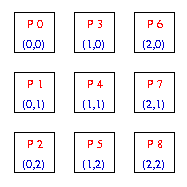
\includegraphics{topo}


\subsection{Cluster Information }

The following functions can be used to obtain information like number
of nodes that the program is running on, node ID of the process, and
other cluster information as discussed below:

The function
\begin{verbatim}
\textcolor{blue}{Fortran}~integer~function~\href{http://www.emsl.pnl.gov/docs/global/ga_ops.html\#ga_cluster_nnodes}{ga\_{}cluster\_{}nnodes}()~

\textcolor{blue}{C}~~~~~~~int~\href{http://www.emsl.pnl.gov/docs/global/c_nga_ops.html\#ga_cluster_nnodes}{GA\_{}Cluster\_{}nnodes}()~

\textcolor{blue}{C++}~~~~~int~GA::GAServices::clusterNnodes()
\end{verbatim}
returns the total number of nodes that the program is running on.
On SMP architectures, this will be less than or equal to the total
number of processors.

The function
\begin{verbatim}
\textcolor{blue}{Fortran}~integer~function~\href{http://www.emsl.pnl.gov/docs/global/ga_ops.html\#ga_cluster_nodeid}{ga\_{}cluster\_{}nodeid}()~

\textcolor{blue}{C}~~~~~~~int~\href{http://www.emsl.pnl.gov/docs/global/c_nga_ops.html\#ga_cluster_nodeid}{GA\_{}Cluster\_{}nodeid}()~

\textcolor{blue}{C++}~~~~~int~GA::GAServices::clusterNodeid()
\end{verbatim}
returns the node ID of the process. On SMP architectures with more
than one processor per node, several processes may return the same
node id.

The function
\begin{verbatim}
\textcolor{blue}{Fortran}~integer~function~\href{http://www.emsl.pnl.gov/docs/global/ga_ops.html\#ga_cluster_nprocs}{ga\_{}cluster\_{}nprocs}(inode)

\textcolor{blue}{C}~~~~~~~int~\href{http://www.emsl.pnl.gov/docs/global/c_nga_ops.html\#ga_cluster_nprocs}{GA\_{}Cluster\_{}nprocs}(int~inode)~

\textcolor{blue}{C++~~~~}~int~GA::GAServices::clusterNprocs(int~inode)
\end{verbatim}
returns the number of processors available on node inode.

The function
\begin{verbatim}
\textcolor{blue}{Fortran}~integer~function~\href{http://www.emsl.pnl.gov/docs/global/ga_ops.html\#ga_cluster_procid}{ga\_{}cluster\_{}procid}(inode,~iproc)~

\textcolor{blue}{C}~~~~~~~int~\href{http://www.emsl.pnl.gov/docs/global/c_nga_ops.html\#ga_cluster_procid}{GA\_{}Cluster\_{}procid}(int~inode,~int~iproc)~

\textcolor{blue}{C++}~~~~~int~GA::GAServices::clusterProcid(int~inode,~int~iproc)
\end{verbatim}
returns the processor id associated with node inode and the local
processor id iproc. If node inode has N processors, then the value
of iproc lies between 0 and N-1.

\textit{\underbar{Example:}} 2 nodes with 4 processors each. Say,
there are 7 processes created. Assume 4 processes on node 0 and 3
processes on node 1. In this case: number of nodes=2, node id is either
0 or 1 (for example, nodeid of process 2 is 0), number of processes
in node 0 is 4 and node 1 is 3. The global rank of each process is
shown in the figure and also the local rank (rank of the process within
the node.i.e., \texttt{cluster\_procid}) is shown in the parenthesis.

\begin{flushleft}
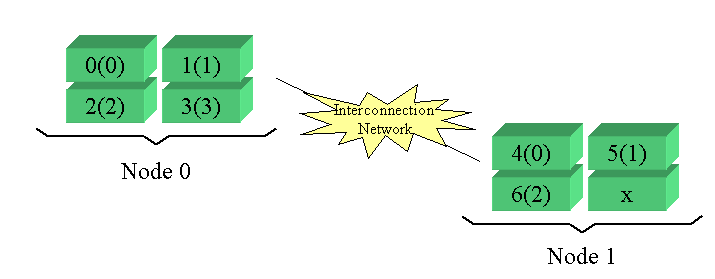
\includegraphics[width=4in]{cluster}
\par\end{flushleft}


\section{Memory Availability }

Even though the memory management does not have to be performed directly
by the user, Global Arrays provide functions to verify the memory
availability. Global Arrays provide the following information:
\begin{enumerate}
\item How much memory has been used by the allocated global arrays. 
\item How much memory is left for allocation of new the global arrays. 
\item Whether the memory in global arrays comes from the \href{http://www.emsl.pnl.gov/docs/parsoft/ma/MAapi.html}{Memory Allocator (MA)}. 
\item Is there any limitation for the memory usage by the Global Arrays.
\end{enumerate}
The function
\begin{verbatim}
\textcolor{blue}{Fortran~}integer~function~\href{http://www.emsl.pnl.gov/docs/global/ga_ops.html\#ga_inquire_memory}{ga\_{}inquire\_{}memory}()~

\textcolor{blue}{C}~~~~~~~size\_t~\href{http://www.emsl.pnl.gov/docs/global/c_nga_ops.html\#ga_inquire_memory}{GA\_{}Inquire\_{}memory}()~

\textcolor{blue}{C++~}~~~~size\_t~GA::GAServices::inquireMemory()
\end{verbatim}
answers the first question. It returns the amount of memory (in bytes)
used in the allocated global arrays on the calling processor.

The function
\begin{verbatim}
\textcolor{blue}{Fortran}~integer~function~\href{http://www.emsl.pnl.gov/docs/global/ga_ops.html\#ga_memory_avail}{ga\_{}memory\_{}avail}()~

\textcolor{blue}{C}~~~~~~~size\_t~\href{http://www.emsl.pnl.gov/docs/global/c_nga_ops.html\#ga_memory_avail}{GA\_{}Memory\_{}avail}()~

\textcolor{blue}{C++}~~~~~size\_t~GA::GAServices::memoryAvailable()
\end{verbatim}
answers the second question. It returns the amount of memory (in bytes)
left for allocation of new global arrays on the calling processor.

\href{http://www.emsl.pnl.gov/docs/parsoft/ma/MAapi.html}{Memory Allocator (MA)}
is a library of routines that comprises a dynamic memory allocator
for use by C, Fortran, or mixed-language applications. Fortran- 77
applications require such a library because the language does not
support dynamic memory allocation. C (and Fortran-90) applications
can benefit from using MA instead of the ordinary malloc() and free()
routines because of the extra features MA provides. The function
\begin{verbatim}
\textcolor{blue}{Fortran}~logical~function~\href{http://www.emsl.pnl.gov/docs/global/ga_ops.html\#ga_uses_ma}{ga\_{}uses\_{}ma}()~

\textcolor{blue}{C}~~~~~~~int~\href{http://www.emsl.pnl.gov/docs/global/c_nga_ops.html\#ga_uses_ma}{GA\_{}Uses\_{}ma}()~

\textcolor{blue}{C++}~~~~~int~GA::GAServices::usesMA()
\end{verbatim}
tells whether the memory in Global Arrays comes from the Memory Allocator
(MA) or not.

The function
\begin{verbatim}
\textcolor{blue}{Fortran}~logical~function~\href{http://www.emsl.pnl.gov/docs/global/ga_ops.html\#ga_memory_limited}{ga\_{}memory\_{}limited}()~

\textcolor{blue}{C}~~~~~~~int~\href{http://www.emsl.pnl.gov/docs/global/c_nga_ops.html\#ga_memory_limited}{GA\_{}Memory\_{}limited}()~

\textcolor{blue}{C++}~~~~~int~GA::GAServices::memoryLimited()
\end{verbatim}
Indicates if a limit is set on memory usage in Global Arrays on the
calling processor. 


\section{Message-Passing Wrappers to Reduce/Broadcast Operations }

Global Arrays provide convenient operations for broadcast/reduce regardless
of the message-passing library the process is running with.

The function
\begin{verbatim}
\textcolor{blue}{Fortran}~subroutine~\href{http://www.emsl.pnl.gov/docs/global/ga_ops.html\#ga_brdcst}{ga\_{}brdcst}(type,~buf,~lenbuf,~root)~

\textcolor{blue}{C}~~~~~~~void~\href{http://www.emsl.pnl.gov/docs/global/c_nga_ops.html\#ga_brdcst}{GA\_{}Brdcst}(void~{*}buf,~int~lenbuf,~int~root)~

\textcolor{blue}{C++}~~~~~void~GA::GAServices::brdcst(void~{*}buf,~int~lenbuf,~int~root)
\end{verbatim}
broadcasts from process root to all other processes a message buffer
of length lenbuf.

The functions
\begin{verbatim}
\textcolor{blue}{Fortran}~subroutine~\href{http://www.emsl.pnl.gov/docs/global/ga_ops.html\#ga_igop}{ga\_{}igop}(type,~x,~n,~op)~

~~~~~~~~subroutine~\href{http://www.emsl.pnl.gov/docs/global/ga_ops.html\#ga_igop}{ga\_{}dgop}(type,~x,~n,~op)~

\textcolor{blue}{C}~~~~~~~void~\href{http://www.emsl.pnl.gov/docs/global/c_nga_ops.html\#ga_igop}{GA\_{}Igop}(long~x{[}{]},~int~n,~char~{*}op)~

~~~~~~~~void~\href{http://www.emsl.pnl.gov/docs/global/c_nga_ops.html\#ga_dgop}{GA\_{}Dgop}(double~x{[}{]},~int~n,~char~{*}op)~

\textcolor{blue}{C++}~~~~~void~GA::GAServices::igop(long~x{[}{]},~int~n,~char~{*}op)~

~~~~~~~~void~GA::GAServices::dgop(double~x{[}{]},~int~n,~char~{*}op)
\end{verbatim}
'sum' elements of \emph{X(1:N)} (a vector present on each process)
across all nodes using the communicative operator \texttt{op}, The
result is broadcasted to all nodes. Supported operations include
\begin{verbatim}
\textbf{+,~{*},~Max,~min,~Absmax,~absmin}
\end{verbatim}
The integer version also includes the \texttt{\textbf{bitwise OR }}operation.

These operations unlike \texttt{ga\_sync}, do not include embedded
\texttt{ga\_gence} operations. 


\section{Others }

There are some other useful functions in Global Arrays. One group
is about inquiring the array attributes. Another group is about printing
the array or part of the array. 


\subsection{Inquire }

A global array is represented by a handle. Given a handle, one can
get the array information, such as the array name, memory used, array
data type, and array dimension information, with the help of the following
functions.

The functions
\begin{verbatim}
\textcolor{green}{n-D}~\textcolor{blue}{Fortran}~subroutine~\href{http://www.emsl.pnl.gov/docs/global/ga_ops.html\#ga_inquire}{nga\_{}inquire}(g\_a,~type,~ndim,~dims)~

\textcolor{green}{2-D}~\textcolor{blue}{Fortran}~subroutine~\href{http://www.emsl.pnl.gov/docs/global/ga_ops.html\#ga_inquire}{nga\_{}inquire}(g\_a,~type,~dim1,~dim2)~

\textcolor{blue}{C}~~~~~~~~~~~void~\href{http://www.emsl.pnl.gov/docs/global/c_nga_ops.html\#ga_inquire}{NGA\_{}Inquire}(int~g\_a,~int~{*}type,~int~

~~~~~~~~~~~~~~~~~~~~{*}ndim,~int~dims{[}{]})~

\textcolor{blue}{C++}~~~~~~~~~void~GA::GlobalArray::inquire(int~{*}type,~int~

~~~~~~~~~~~~~~~~~~~~{*}ndim,~int~dims{[}{]})
\end{verbatim}
return the data type of the array, and also the dimensions of the
array.

The function
\begin{verbatim}
\textcolor{blue}{Fortran}~subroutine~\href{http://www.emsl.pnl.gov/docs/global/ga_ops.html\#ga_inquire_name}{ga\_{}inquire\_{}name}(g\_a,~array\_name)~

\textcolor{blue}{C}~~~~~~~char{*}~\href{http://www.emsl.pnl.gov/docs/global/c_nga_ops.html\#ga_inquire_name}{GA\_{}Inquire\_{}name}(int~g\_a)~~

\textcolor{blue}{C++}~~~~~char{*}~GA::GlobalArray::inquireName()
\end{verbatim}
finds out the name of the array.

One can also inquire the memory being used with \texttt{ga\_inquire\_memory}
(discussed above). 


\subsection{Print }

Global arrays provide functions to print
\begin{enumerate}
\item content of the global array 
\item content of a patch of global array 
\item the status of array operations 
\item a summary of allocated arrays
\end{enumerate}
The function
\begin{verbatim}
\textcolor{blue}{Fortran}~subroutine~\href{http://www.emsl.pnl.gov/docs/global/ga_ops.html\#ga_print}{ga\_{}print}(g\_a)~

\textcolor{blue}{C}~~~~~~~void~\href{http://www.emsl.pnl.gov/docs/global/c_nga_ops.html\#ga_print}{GA\_{}Print}(int~g\_a)~

\textcolor{blue}{C++}~~~~~void~GA::GlobalArray::print()
\end{verbatim}
prints the entire array to the standard output. The output is formatted.

A utility function is provided to print data in the patch, which is
\begin{verbatim}
\textcolor{blue}{Fortran}~subroutine~\href{http://www.emsl.pnl.gov/docs/global/ga_ops.html\#ga_print_patch}{nga\_{}print\_{}patch}(g\_a,~lo,~hi,~pretty)~

\textcolor{blue}{C}~~~~~~~void~\href{http://www.emsl.pnl.gov/docs/global/c_nga_ops.html\#ga_print_patch}{NGA\_{}Print\_{}patch}(int~g\_a,~int~lo{[}{]},~

~~~~~~~~~~~~~~~~~~~int~hi{[}{]},~int~pretty)~

\textcolor{blue}{C++}~~~~~void~GA::GlobalArray::printPatch(int~lo{[}{]},~

~~~~~~~~~~~~~~~~~~~int~hi{[}{]},~int~pretty)
\end{verbatim}
One can either specify a formatted output (set \texttt{pretty} to
one) where the output is formatted and rows/ columns are labeled,
or (set \texttt{pretty} to zero) just dump all the elements of this
patch to the standard output without any formatting.

The function
\begin{verbatim}
\textcolor{blue}{Fortran}~subroutine~\href{http://www.emsl.pnl.gov/docs/global/ga_ops.html\#ga_print_stats}{ga\_{}print\_{}stats}()~

\textcolor{blue}{C}~~~~~~~void~\href{http://www.emsl.pnl.gov/docs/global/c_nga_ops.html\#ga_print_stats}{GA\_{}Print\_{}stats}()~

\textcolor{blue}{C++}~~~~~void~GA::GAServices::printStats()
\end{verbatim}
prints the global statistics information about array operations for
the calling process, including
\begin{itemize}
\item number of calls to the GA create/duplicate, destroy, get, put, scatter,
gather, and read\_and\_inc operations 
\item total amount of data moved in the GA primitive operations 
\item amount of data moved in GA primitive operations to logically remote
locations 
\item maximum memory consumption in global arrays, the \textquotedbl{}high-water
mark\textquotedbl{}
\end{itemize}
The function
\begin{verbatim}
\textcolor{blue}{Fortran}~subroutine~\href{http://www.emsl.pnl.gov/docs/global/ga_ops.html\#ga_print_distribution}{ga\_{}print\_{}distribution}(g\_a)~

\textcolor{blue}{C~}~~~~~~void~\href{http://www.emsl.pnl.gov/docs/global/c_nga_ops.html\#ga_print_distribution}{GA\_{}Print\_{}distribution}(int~g\_a)

\textcolor{blue}{C}~~~~~~~void~GA::GlobalArray::printDistribution()
\end{verbatim}
prints the global array distribution. It shows mapping array data
to the processes.

The function
\begin{verbatim}
\textcolor{blue}{Fortran}~subroutine~\href{http://www.emsl.pnl.gov/docs/global/ga_ops.html\#ga_summarize}{ga\_{}summarize}(verbose)~

\textcolor{blue}{C~}~~~~~~void~\href{http://www.emsl.pnl.gov/docs/global/c_nga_ops.html\#ga_summarize}{GA\_{}Summarize}(int~verbose)~

\textcolor{blue}{C++}~~~~~void~GA::GAServices::summarize(int~verbose)
\end{verbatim}
prints info about allocated arrays. verbose can be either one or zero. 


\subsection{Miscellaneous }

The function
\begin{verbatim}
\textcolor{blue}{Fortran}~subroutine~\href{http://www.emsl.pnl.gov/docs/global/ga_ops.html\#ga_check_handle}{ga\_{}check\_{}handle}(g\_a,~string)~

\textcolor{blue}{C~~}~~~~~void~\href{http://www.emsl.pnl.gov/docs/global/c_nga_ops.html\#ga_check_handle}{GA\_{}Check\_{}handle}(int~g\_a,~char~{*}string)

\textcolor{blue}{C++}~~~~~void~GA::GlobalArray::checkHandle(char~{*}string)
\end{verbatim}
checks if the global array handle \texttt{g\_a} represents a valid
array. The \texttt{string} is the message to be printed when the handle
is invalid.


\chapter{GA++: C++ Bindings for Global Arrays}

\chapter{GA++: C++ Bindings for Global Arrays}

\section{Overview }

GA++ provides a C++ interface to global arrays (GA) libraries. The
doxygen documentation of GA++ is located here: \href{http://www.emsl.pnl.gov/docs/global/ga++/index.html}{http://www.emsl.pnl.gov/docs/global/ga++/index.html}.
The GA C++ bindings are a layer built directly on top of the GA C
bindings. GA++ provides new names for the C bindings of GA functions
(For example, GA\_Add\_patch() is renamed as addPatch()). 


\section{GA++ Classes }

All GA classes (GAServices, GlobalArray) are declared within the scope
of GA namespace.

\textbf{\textcolor{black}{Namespace issue: }}Although namespace is
part of the ANSI C++ standard, not all C++ compilers support namespaces
(A non-instantiable GA class is provided for implementations using
compilers without namespace). \textbf{Note}: define the variable \_GA\_USENAMESPACE\_
as 0 in ga++.h if your compiler does not support namespaces. 
\begin{verbatim}
namespace~GA~\{

~~~~~~class~GAServices;~

~~~~~~class~GlobalArray;~

\};
\end{verbatim}
The current implementation has no derived classes (no (virtual) inheritance),
templates, or exception handling. Eventually, more object oriented
functionalities will be added, and standard library facilities will
be used without affecting the performance. 


\section{Initialization and Termination: }

GA namespace has the following static functions for initialization
and termination of Global Arrays.

GA::Initialize(): Initialize Global Arrays, allocates and initializes
internal data structures in Global Arrays. This is a collective operation.

GA::Terminate(): Delete all active arrays and destroy internal data
structures. This is a collective operation.

namespace GA \{ \_GA\_STATIC\_ void Initialize(int argc, char {*}argv{[}{]},
size\_t limit = 0); \_GA\_STATIC\_ void Initialize(int argc, char
{*}argv{[}{]}, unsigned long heapSize, unsigned long stackSize, int
type, size\_t limit = 0); \_GA\_STATIC\_ void Terminate(); \};

\emph{\underbar{Example}}: 

\#include <iostream.h> \#include \textquotedbl{}ga++.h\textquotedbl{}

int main(int argc, char {*}{*}argv) \{ GA::Initialize(argc, argv,
0); cout <\textcompwordmark{}< \textquotedbl{}Hello World\textbackslash{}n\textquotedbl{};
GA::Terminate(); \} 


\section{GAServices}

GAServices class has member functions that does all the global operations
(non-array operations) like Process Information (number of processes,
process id, ..), Inter-process Synchronization (sync, lock, broadcast,
reduce,..), etc,.

SERVICES Object: GA namespace has a global \textquotedbl{}SERVICES\textquotedbl{}
object (of type \textquotedbl{}GAServices\textquotedbl{}), which can
be used to invoke the non-array operations. To call the functions
(for example, sync()), we invoke them on this SERVICES object (for
example, GA::SERVICES.sync()). As this object is in the global address
space, the functions can be invoked from anywhere inside the program
(provided the ga++.h is included in that file/program). 


\section{Global Array}

GlobalArray class has member functions that perform:

{*} Array operations {*} One-sided (get/put), {*} Collective array
operations, {*} Utility operations, etc,. 


\chapter{Mirrored Arrays}


\section{Overview}

Mirrored arrays use a hybrid approach to replicate data across cluster
nodes and distribute data within each node. It uses shared memory
for caching latency sensitive distributed data structures on Symmetric
Multi-Processor nodes of clusters connected with commodity networks
as illustrated in Figure~\ref{cap:2-D-Array}. The user is responsible
for managing consistency of the data cached within the mirrored arrays.
Instead of applying mirroring to all distributed arrays, the user
can decide, depending on the nature of the algorithm and the communication
requirements (number and size of messages), which arrays can or should
use mirroring and which should be left fully distributed and accessed
without the shared memory cache. 

This hybrid approach is particularly useful for problems where it
is important to solve a moderate sized problem many times, such as
an ab initio molecular dynamics simulation of a moderate size molecule.
A single calculation of the energy and forces that can be run in a
few minutes may be suitable for a geometry optimization, where a few
tens of calculations are required, but is still too long for a molecular
dynamics trajectory, which can require tens of thousands of separate
evaluations. For these problems, it is still important to push scalability
to the point where single energy and force calculations can be performed
on the order of seconds. Similar concerns exist for problems involving
Monte Carlo sampling or sensitivity analysis where it is important
to run calculations quickly so that many samples can be taken.

Mirrored arrays differ from traditional replicated data schemes in
two ways. First, mirrored arrays can be used in conjunction with distributed
data and there are simple operations that support conversion back
and forth from mirrored to distributed arrays. This allows developers
maximum flexibility in incorporating mirrored arrays into their algorithms.
Second, mirrored arrays are distributed within an SMP node (see the
above figure). For systems with a large number of processors per node,
e.g., 32 in the current generation IBM SP, this can result in significant
distribution of the data. Even for systems with only 2 nodes per processor,
this will result in an immediate savings of 50\% over a conventional
replicated data scheme.

%
\begin{figure}
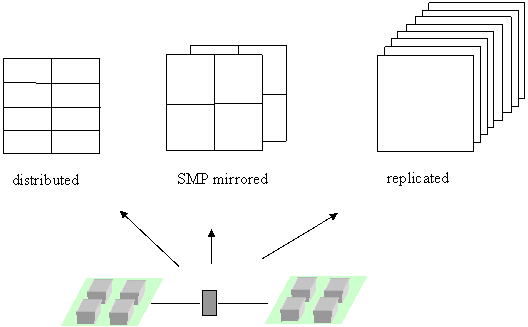
\includegraphics[width=0.9\columnwidth]{mirrored}

\caption{\label{cap:2-D-Array}Example of a two-dimensional array fully distributed,
SMP mirrored, and replicated on two 4-way SMP cluster nodes. }

\end{figure}


The disadvantage of using mirrored arrays is that problems are limited
in size by what can fit onto a single SMP node. This can be partially
offset by the fact that almost all array operations can be supported
on both mirrored and distributed arrays, so that it is easy to develop
code that can switch between using mirrored arrays and conventional
distributed arrays, depending on problem size and the number of available
processors.


\section{Mirrored Array Operations}
\begin{lyxcode}
Fortran~integer~\href{http://www.emsl.pnl.gov/docs/global/ga_ops.html\#GA_PGROUP_GET_MIRROR}{ga\_{}pgroup\_{}get\_{}mirror}()~

C~~~~~~~int~\href{http://www.emsl.pnl.gov/docs/global/c_nga_ops.html\#GA_PGROUP_GET_MIRROR}{ga\_{}pgroup\_{}get\_{}mirror}()~

C++~~~~~int~GA::GAServices::pgroupGetMirror()
\end{lyxcode}
This function returns a handle to the mirrored processor list, which
can then be used to create a mirrored global array using one of the
NGA\_Create\_{*}\_config calls.
\begin{lyxcode}
Fortran~integer~\href{http://www.emsl.pnl.gov/docs/global/ga_ops.html\#GA_MERGE_MIRRORED}{ga\_{}merge\_{}mirrored}(g\_a)~

C~~~~~~~int~\href{http://www.emsl.pnl.gov/docs/global/c_nga_ops.html\#GA_MERGE_MIRRORED}{GA\_{}Merge\_{}mirrored}(int~g\_a)~

C++~~~~~int~GA::GlobalArray::mergeMirrored()
\end{lyxcode}
This subroutine merges mirrored arrays by adding the contents of each
array across nodes. The result is that the each mirrored copy of the
array represented by g\_a is the sum of the individual arrays before
the merge operation. After the merge, all mirrored arrays are equal.
This is a collective operation.
\begin{lyxcode}
Fortran~integer~\href{http://www.emsl.pnl.gov/docs/global/ga_ops.html\#GA_MERGE_DISTR_PATCH}{nga\_{}merge\_{}distr\_{}patch}(g\_a,~alo,~ahi,~

~~~~~~~~~~~~~~~~g\_b,~blo,~bhi)~

C~~~~~~~int~\href{http://www.emsl.pnl.gov/docs/global/c_nga_ops.html\#GA_MERGE_DISTR_PATCH}{NGA\_{}Merge\_{}distr\_{}patch}(int~g\_a,~int~alo{[}{]},~

~~~~~~~~~~~~~~~~int~ahi{[}{]},~int~g\_b,~int~blo{[}{]},~int~bhi{[}{]})~

C++~~~~~int~GA::GlobalArray::mergeDistrPatch(int~alo{[}{]},~

~~~~~~~~~~~~~~~~int~ahi{[}{]},~int~g\_b,~int~blo{[}{]},~int~bhi{[}{]})
\end{lyxcode}
This function merges all copies of a patch of a mirrored array (g\_a)
into a patch in a distributed array (g\_b). This is same as GA\_merge\_mirrored,
except, this function is operated on a patch rather than the whole
array. This is a collective operation.
\begin{lyxcode}
Fortran~integer~\href{http://www.emsl.pnl.gov/docs/global/ga_ops.html\#ga_is_mirrored}{ga\_{}is\_{}mirrored}(g\_a)~

C~~~~~~~int~\href{http://www.emsl.pnl.gov/docs/global/c_nga_ops.html\#ga_is_mirrored}{GA\_{}Is\_{}mirrored}(int~g\_a)~

C++~~~~~int~GA::GlobalArray::isMirrored()
\end{lyxcode}
This subroutine checks if the array is mirrored array or not. Returns
1 if it is a mirrored array, else it returns 0. This is a local operation. 


\chapter{Processor Groups}

\chapter{Processor Groups}

\section{Overview}

The Global Arrays toolkit has recently been extended to support global
arrays defined on processor groups. The processor groups in GA programs
follow the MPI approach. The MPI processor groups can be used in GA
programs. However, since the MPI standard does not support fault tolerance,
GA provides a set of APIs for process group managment which offers
some opportunities for supporting environments with hardware faults.

In general, processor groups allow the programmer to subdivide the
domain containing the complete set of processors (\textquotedblleft{}the
world group\textquotedblright{}) into subsets of processors that can
act more or less independently of one another. Global arrays that
are created on processor groups are only distributed amongst the processors
in the group and not on all processors in the system. Collective operations
executed on specific groups are also restricted to processors in the
group and do not require any action from processors outside the group.
A simple example is a synchronization operation. If the synchronization
operation is executed on a group that is a subgroup of the world group,
then only those processors in the subgroup are blocked until completion
of the synchronization operation. Processors outside the subgroup
can continue their operations without interruption.

The Global Arrays toolkit contains a collection of library calls that
can be used to explicitly create groups, assign specific groups to
global arrays, and execute global operations on groups. There is also
a mechanism for setting the \textquotedblleft{}default\textquotedblright{}
group for the calculation. This is a powerful way of converting large
amounts of parallel code that has already been written using the Global
Arrays library to run as a subroutine on a processor group. Normally,
the default group for a parallel calculation is the world group, but
a call is available that can be used to change the default group to
something else. This call must be executed by all processors in the
subgroup. Furthermore, although it is not required, it is probably
a very good idea to make sure that the default groups for all processors
in the system (i.e., all processors contained in the original world
group) represent a complete non-overlapping covering of the original
world group (see figure). Once the default group has been set, all
operations are implicitly assumed to occur on the default processor
group unless explicitly stated otherwise. Global Arrays are only created
on the default processor group and global operations, such as synchronizations,
broadcasts, and other operations, are restricted to the default group.
Inquiry functions, such as the number of nodes and the node ID, return
values relative to the default processor group. Thus, a call to the
ga\_nodeid function will return a value of 0 for each processor designated
as the zero processor within each default group. The number of processors
returning 0 will be equal to the number of default groups (assuming
the complete non-overlapping coverage suggested above is implemented).

\begin{tabular}{|>{\centering}p{10cm}|}
\hline 
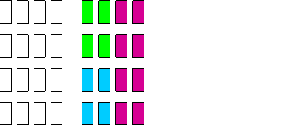
\includegraphics{groups}\tabularnewline
\hline
\hline 
Original set of 16 processors decomposed into 3 non-overlapping groups.\tabularnewline
\hline
\end{tabular}

At present there are not many function calls that support operations
between groups. The only calls that can be used to copy data from
one group to another are the \texttt{nga\_copy} and \texttt{nga\_copy\_patc}h
calls. These can be used to copy global arrays between two groups,
provided that one group is completely contained in the other (this
will always be the case if one of the groups is the world group).
These commands will work correctly as long as they are executed only
by processors contained in the smaller group. The \texttt{nga\_put}
and \texttt{nga\_get} commands can also be used to communicate between
Global Arrays on different groups (using an intermediate buffer),
provided that the two groups share at least one processor (again,
this will always be the case if one group is the world group).

The new functions included in the Global Arrays library are described
below. 


\section{Creating New Groups}
\begin{verbatim}
\textcolor{blue}{Fortran}~integer~function~\href{http://www.emsl.pnl.gov/docs/global/ga_ops.html\#GA_PGROUP_CREATE}{ga\_{}pgroup\_{}create}(list,~size)

\textcolor{blue}{C}~~~~~~~int~\href{http://www.emsl.pnl.gov/docs/global/c_nga_ops.html\#GA_PGROUP_CREATE}{GA\_{}Pgroup\_{}create}(int~{*}list,~int~size)
\end{verbatim}
This call can be used to create a processor group of size \texttt{size}
containing the processors in the array \texttt{list}. This call must
be executed on all processors in the group. It returns an integer
handle (for the processors group) that can be used to reference the
processor group in other library calls.

Assigning groups:
\begin{verbatim}
\textcolor{blue}{Fortran}~subroutine~\href{http://www.emsl.pnl.gov/docs/global/ga_ops.html\#GA_SET_PGROUP}{ga\_{}set\_{}pgroup}(g\_a,~p\_handle)

\textcolor{blue}{C}~~~~~~~void~\href{http://www.emsl.pnl.gov/docs/global/c_nga_ops.html\#GA_SET_PGROUP}{GA\_{}Set\_{}pgroup}(int~g\_a,~int~p\_handle)
\end{verbatim}
This call can be used to assign the processor group \texttt{p\_handle}
to a global array handle \texttt{g\_a} that has been previously created
using the \texttt{ga\_create\_handle} call. The processor group associated
with a global array can also be set by creating the global array with
one of the \texttt{nga\_create\_XXX\_config} calls. 


\section{Setting the Default Group}
\begin{verbatim}
\textcolor{blue}{Fortran}~subroutine~\href{http://www.emsl.pnl.gov/docs/global/ga_ops.html\#GA_PGROUP_SET_DEFAULT}{ga\_{}pgroup\_{}set\_{}default}(p\_handle)

\textcolor{blue}{C}~~~~~~~void~\href{http://www.emsl.pnl.gov/docs/global/c_nga_ops.html\#GA_PGROUP_SET_DEFAULT}{GA\_{}Pgroup\_{}set\_{}default}(int~p\_handle)
\end{verbatim}
This call can be used to set the default group to something besides
the world group. This call must be made on all processors contained
in the group represented by \texttt{p\_handle}. Once the default group
has been set, all operations are restricted to the default group unless
explicitly stated otherwise. 


\section{Inquiry functions}
\begin{verbatim}
\textcolor{blue}{Fortran}~integer~function~\href{http://www.emsl.pnl.gov/docs/global/ga_ops.html\#GA_PGROUP_NNODES}{ga\_{}pgroup\_{}nnodes}(p\_handle)

\textcolor{blue}{C}~~~~~~~int~\href{http://www.emsl.pnl.gov/docs/global/c_nga_ops.html\#GA_PGROUP_NNODES}{GA\_{}Pgroup\_{}nnodes}(int~p\_handle)

\textcolor{blue}{Fortran}~integer~function~\href{http://www.emsl.pnl.gov/docs/global/ga_ops.html\#GA_PGROUP_NODEID}{ga\_{}pgroup\_{}nodeid}(p\_handle)

\textcolor{blue}{C}~~~~~~~int~\href{http://www.emsl.pnl.gov/docs/global/c_nga_ops.html\#GA_PGROUP_NODEID}{GA\_{}Pgroup\_{}nodeid}(int~p\_handle)
\end{verbatim}
These functions can be used to access information about the group.
The \texttt{ga\_pgroup\_nnodes} function returns the number of processors
in the group specified by the handle \texttt{p\_handle}, \texttt{ga\_pgroup\_nodeid}
returns the local node ID of the processor within the group.
\begin{verbatim}
\textcolor{blue}{Fortran}~integer~function~\href{http://www.emsl.pnl.gov/docs/global/ga_ops.html\#GA_PGROUP_GET_DEFAULT}{ga\_{}pgroup\_{}get\_{}default}()

\textcolor{blue}{C}~~~~~~~int~\href{http://www.emsl.pnl.gov/docs/global/c_nga_ops.html\#GA_PGROUP_GET_DEFAULT}{GA\_{}Pgroup\_{}get\_{}default}()

\textcolor{blue}{Fortran}~integer~function~\href{http://www.emsl.pnl.gov/docs/global/ga_ops.html\#GA_PGROUP_GET_MIRROR}{ga\_{}pgroup\_{}get\_{}mirror}()

\textcolor{blue}{C}~~~~~~~int~\href{http://www.emsl.pnl.gov/docs/global/c_nga_ops.html\#GA_PGROUP_GET_MIRROR}{GA\_{}Pgroup\_{}get\_{}mirror}()

\textcolor{blue}{Fortran}~integer~function~\href{http://www.emsl.pnl.gov/docs/global/ga_ops.html\#GA_PGROUP_GET_WORLD}{ga\_{}pgroup\_{}get\_{}world}()

\textcolor{blue}{C}~~~~~~~int~\href{http://www.emsl.pnl.gov/docs/global/c_nga_ops.html\#GA_PGROUP_GET_WORLD}{GA\_{}Pgroup\_{}get\_{}world}()
\end{verbatim}
These functions can be used to get the handles for some standard groups
at any point in the program. This is particularly useful for gaining
access to the world group if the default group has been reset to a
subgroup and also for gaining access to the handle for the mirror
group (see section on mirrored arrays). Note that the mirror group
is actually a group defined on the complete set of processors. 


\section{Collective operations on groups}
\begin{verbatim}
\textcolor{blue}{Fortran}~subroutine~\href{http://www.emsl.pnl.gov/docs/global/ga_ops.html\#GA_PGROUP_SYNC}{ga\_{}pgroup\_{}sync}(p\_handle)

\textcolor{blue}{C}~~~~~~~void~\href{http://www.emsl.pnl.gov/docs/global/ga_ops.html\#GA_PGROUP_SYNC}{ga\_{}pgroup\_{}sync}(p\_handle)

\textcolor{blue}{Fortran}~subroutine~\href{http://www.emsl.pnl.gov/docs/global/ga_ops.html\#GA_PGROUP_BRDCST}{ga\_{}pgroup\_{}brdcst}(p\_handle,type,

~~~~~~~~~~~~~~~~~~~buf,lenbuf,root)

\textcolor{blue}{C}~~~~~~~void~\href{http://www.emsl.pnl.gov/docs/global/ga_ops.html\#GA_PGROUP_BRDCST}{GA\_{}Pgroup\_{}brdcst}(int~p\_handle,~void~

~~~~~~~~~~~~~~~~~~~{*}buf,~root)

\textcolor{blue}{Fortran}~subroutine~\href{http://www.emsl.pnl.gov/docs/global/ga_ops.html\#GA_PGROUP_DGOP}{ga\_{}pgroup\_{}dgop}(p\_handle,~type,~

~~~~~~~~~~~~~~~~~~~buf,~lenbuf,~op)

\textcolor{blue}{Fortran}~subroutine~\href{http://www.emsl.pnl.gov/docs/global/ga_ops.html\#GA_PGROUP_SGOP}{ga\_{}pgroup\_{}sgop}(p\_handle,~type,~

~~~~~~~~~~~~~~~~~~~buf,~lenbuf,~op)

\textcolor{blue}{Fortran}~subroutine~\href{http://www.emsl.pnl.gov/docs/global/ga_ops.html\#GA_PGROUP_IGOP}{ga\_{}pgroup\_{}igop}(p\_handle,~type,~

~~~~~~~~~~~~~~~~~~~buf,~lenbuf,~op)

\textcolor{blue}{C}~~~~~~~void~\href{http://www.emsl.pnl.gov/docs/global/c_nga_ops.html\#GA_PGROUP_DGOP}{GA\_{}Pgroup\_{}dgop}(int~p\_handle,~double~

~~~~~~~~~~~~~~~~~~~{*}buf,~int~lenbuf,~char~{*}op)

\textcolor{blue}{C}~~~~~~~void~\href{http://www.emsl.pnl.gov/docs/global/c_nga_ops.html\#GA_PGROUP_FGOP}{GA\_{}Pgroup\_{}fgop}(int~p\_handle,~float~

~~~~~~~~~~~~~~~~~~~{*}buf,~int~lenbuf,~char~{*}op)

\textcolor{blue}{C}~~~~~~~void~\href{http://www.emsl.pnl.gov/docs/global/c_nga_ops.html\#GA_PGROUP_IGOP}{GA\_{}Pgroup\_{}igop}(int~p\_handle,~int~

~~~~~~~~~~~~~~~~~~~{*}buf,~int~lenbuf,~char~{*}op)

\textcolor{blue}{C}~~~~~~~void~\href{http://www.emsl.pnl.gov/docs/global/c_nga_ops.html\#GA_PGROUP_LGOP}{GA\_{}Pgroup\_{}lgop}(int~p\_handle,~long~

~~~~~~~~~~~~~~~~~~~{*}buf,~int~lenbuf,~char~{*}op)
\end{verbatim}
These operations are all identical to the standard global operations,
the only difference is that they have an extra argument that takes
a group handle. The action of these calls is restricted to the set
of processors contained in the group represented by \texttt{p\_handle}.
All processors in the group must call these subroutines.


\chapter{Sparse Data Operations}

\chapter{Sparse Data Operations}

The Global Arrays Toolkit contains several subroutines designed to
support operations on sparse data sets. Most sparse data objects,
such as sparse matrices, are generally described using a collection
of 1-dimensional arrays, so the operations discussed below are primarily
focused on 1D Global Arrays. The discussion of sparse data operations
will begin by describing the sparse data subroutines and then will
show how they can be used by describing an algorithm for doing a sparse
matrix-dense vector multiply.
\begin{verbatim}
Fortran~subroutine~ga\_patch\_enum(g\_a,~lo,~hi,~istart,~istride)~

C~~~~~~~void~GA\_Patch\_enum(int~g\_a,~int~lo,~int~hi,~

~~~~~~~~~~~~~~~~~~~~~~~~~~~int~istart,~int~istride)
\end{verbatim}
This subroutine enumerates the elements of an array between elements
\texttt{lo} and \texttt{hi} starting with the value istart and incrementing
each subsequent value by \texttt{istride}. This is a collective operation.
Some examples of its use are shown below:
\begin{verbatim}
call~ga\_patch\_enum(g\_a,~1,~n,~1,~1)~

g\_a:~1~2~3~4~5~6~7~8~9~10~...~n

call~ga\_zero(g\_a)~

call~ga\_patch\_enum(g\_a,~5,~n,~7,~2)~

g\_a:~0~0~0~0~7~9~11~13~15~...

Fortran~subroutine~ga\_scan\_copy(g\_src,~g\_dest,~g\_mask,~lo,~hi)~

C~~~~~~~void~GA\_Scan\_copy(int~g\_src,~int~g\_dest,~int~g\_mask,~

~~~~~~~~~~~~~~~~~~~~~~~~~~int~lo,~int~hi)
\end{verbatim}
This subroutine does a segmented scan-copy of values in the source
array \texttt{g\_src} into a destination array \texttt{g\_dest} with
segments defined by values in an integer mask array \texttt{g\_mask}.
The scan-copy operation is only applied to the range between the \texttt{lo}
and \texttt{hi} indices. The resulting destination array will contain
segments of consecutive elements with the same value. This is a collective
operation. An example is shown below to illustrate the behavior of
this operation. 
\begin{verbatim}
call~ga\_scan\_copy(g\_src,~g\_dest,~g\_mask,~1,~n)~

g\_mask:~1~0~0~0~0~1~0~1~0~0~1~0~0~0~1~1~0~

g\_src:~5~8~7~3~2~6~9~7~3~4~8~2~3~6~9~10~7~

g\_dest:~5~5~5~5~5~6~6~7~7~7~8~8~8~8~9~10~10~



Fortran~subroutine~ga\_scan\_add(g\_src,~g\_dest,~g\_mask,~lo,~hi,~excl)~

C~~~~~~~void~GA\_Scan\_add(int~g\_src,~int~g\_dest,~int~g\_mask,~

~~~~~~~~~~~~~~~~~~~~~~~~~int~lo,~int~hi,~int~excl)
\end{verbatim}
This operation will add successive elements in a source vector \texttt{g\_src
}and put the results in a destination vector \texttt{g\_dest}. The
addition will restart based on the values of the integer mask vector
\texttt{g\_mask}. The scan is performed within the range defined by
the indices \texttt{lo} and \texttt{hi}. The excl flag determines
whether the sum starts with the value in the source vector corresponding
to the location of a 1 in the mask vector (\texttt{excl=0}) or whether
the first value is set equal to 0 (\texttt{excl=1}). Some examples
of this operation are given below.
\begin{verbatim}
call~ga\_scan\_add(g\_src,~g\_dest,~g\_mask,~1,~n,~0)~

g\_mask:~1~0~0~0~0~0~1~0~1~0~0~1~0~0~1~1~0~

g\_src:~1~2~3~4~5~6~7~8~9~10~11~12~13~14~15~16~17~

g\_dest:~1~3~6~10~15~21~7~15~9~19~30~12~25~39~15~16~33



call~ga\_scan\_add(g\_src,~g\_dest,~g\_mask,~1,~n,~1)~

g\_mask:~1~0~0~0~0~0~1~0~1~0~0~1~0~0~1~1~0~

g\_src:~1~2~3~4~5~6~7~8~9~10~11~12~13~14~15~16~17~

g\_dest:~0~1~3~6~10~15~0~7~0~9~19~0~12~25~0~0~16



Fortran~subroutine~ga\_pack(g\_src,~g\_dest,~g\_sbit,~lo,~hi,~icount)~

C~~~~~~~void~GA\_Pack(int~g\_src,~int~g\_dest,~

~~~~~~~~~~~~~~~~~~~~~int~g\_sbit,~int~lo,~int~hi,~int~icount)
\end{verbatim}
The pack routine is designed to compress the values in the source
vector\texttt{ g\_src} into a smaller destination array\texttt{ g\_dest}
based on the values in an integer mask array \texttt{g\_mask}. The
values \texttt{lo} and \texttt{hi} denote the range of elements that
should be compressed and \texttt{icount} is a variable that on output
lists the number of values placed in the compressed array. This is
a collective operation. An example of its use is shown below.
\begin{verbatim}
call~ga\_pack(g\_src,~g\_dest,~g\_mask,~1,~n,~icount)~

g\_mask:~1~0~0~0~0~1~0~1~0~0~1~0~0~0~1~0~0~

g\_src:~1~2~3~4~5~6~7~8~9~10~11~12~13~14~15~16~17~

g\_dest:~1~6~8~11~15~

icount:~5



Fortran~subroutine~ga\_unpack(g\_src,~g\_dest,~g\_sbit,~lo,~hi,~icount)~

C~~~~~~~void~GA\_Pack(int~g\_src,~int~g\_dest,~int~g\_sbit,~

~~~~~~~~~~~~~~~~~~~~~int~lo,~int~hi,~int~icount)
\end{verbatim}
The unpack routine is designed to expand the values in the source
vector \texttt{g\_src} into a larger destination array \texttt{g\_dest}
based on the values in an integer mask array \texttt{g\_mask}. The
values \texttt{lo} and \texttt{hi} denote the range of elements that
should be expanded and icount is a variable that on output lists the
number of values placed in the uncompressed array. This is a collective
operation. An example of its use is shown below.
\begin{verbatim}
call~ga\_unpack(g\_src,~g\_dest,~g\_mask,~1,~n,~icount)~

g\_mask:~1~0~0~0~0~1~0~1~0~0~1~0~0~0~1~0~0~

g\_src:~1~6~8~11~15~

g\_dest:~1~0~0~0~0~6~0~8~0~0~11~0~0~0~15~0~0~

icount:~5
\end{verbatim}

\section{Sparse Matrix-Vector Multiply Example:}

The utility of these subroutines in actual applications is by no means
obvious so to illustrate their use, we describe a simple sparse matrix-vector
multiply. The starting point of this calculation is a compressed sparse
row (CSR) matrix in which only the non-zero elements are stored. The
CSR storage format for an NxN matrix consists of three vectors. The
first is a VALUES vector consisting of all the non-zero values contained
in the matrix, the second is a J-INDEX vector that contains all the
j indices of the values stored in the VALUES vector and the third
vector is the I-INDEX vector that contains N+1 entries and contains
the offsets in the J-INDEX vector corresponding to each row in the
matrix. The last entry in I-INDEX corresponds to the total number
of non-zero values in the sparse matrix. The VALUES and J-INDEX vectors
should contain the same number of elements. Within each row the values
are ordered by increasing values of the j index and then by increasing
values of the i index. An example of a sparse matrix and its CSR representation
is shown below. 
\begin{verbatim}
~~~~~0~0~1~3~0

~~~~~2~0~0~0~5

~~~~~0~7~0~9~0

~~~~~3~0~4~0~5

~~~~~0~2~0~0~6
\end{verbatim}
The CSR representation of this matrix is
\begin{verbatim}
VALUES:~1~3~2~5~7~9~3~4~5~2~6~

J-INDEX:~3~4~1~5~2~4~1~3~5~2~5~

I-INDEX:~1~3~5~7~10~12
\end{verbatim}
Note that each value in I-INDEX corresponds to the location of the
first element of the row in J-INDEX. The last element in I-INDEX equals
one plust the total number of non-zero elements in the matrix and
is a useful number to have available when performing sparse matrix
operations. Depending on indexing conventions, it might be more useful
to set the last element equal to the number of non-zero elements.

For a very large sparse matrix, it may be necessary to distribute
the CSR representation across multiple processors. This example assumes
that the each of the components of the CSR matrix is stored in a 1-dimensional
Global Array. To start the calculation, it is first necessary to create
the distributed CSR matrix. We assume that it is possible to assign
the evaluation of individual rows to individual processors. A simple
way of starting is to divide up the number of rows evenly between
processors and have each processor evaluate all elements of the rows
assigned to it. These can then be stored in a local CSR format. In
this case, the I-INDEX vector contains only the number of rows assigned
to the processor. In the example shown above, assume that the matrix
is divided between three processors and that processes 0 and 1 have
two rows each and process 2 has one row. The layout on the three processes
looks like
\begin{verbatim}
Process~0~

VALUES:~1~3~2~5~

J-INDEX:~3~4~1~5~

I-INDEX:~1~3~

INC:~2~2



Process~1~

VALUES:~7~9~3~4~5~

J-INDEX:~2~4~1~3~5~

I-INDEX:~1~3~

INC:~2~3



Process~2~

VALUES:~2~6~

J-INDEX:~2~5~

I-INDEX:~1~

INC:~2~
\end{verbatim}
The local array INC contains the number of non-zero elements in each
row. The total number of non-zero elements in the matrix can be found
by summing the number of non-zero values on each process. This value
can then be used to create distributed VALUES and J-INDEX arrays containing
the complete CSR matrix. A distributed I-INDEX array can be constructed
from knowledge of the original matrix dimension N. In addition to
Global Arrays representing distributed versions of VALUES, J-INDEX,
and I-INDEX, an integer Global Array of length N+1 called SBIT is
also needed. This array is initialized so that the first element is
1 and the remaining elements are all zero. To create the distributed
array I-INDEX a temporary Global Array of length N+1 is created. The
following code fragment illustrates the construction of I-INDEX
\begin{verbatim}
lo~=~imin~+~1~\textcolor{blue}{!~imin~is~lower~index~of~i~values~on~}

\textcolor{blue}{{}~~~~~~~~~~~~~~!~this~processor~}

hi~=~imax~+~1~\textcolor{blue}{!~imax~is~upper~index~of~i~values~on~}

\textcolor{blue}{{}~~~~~~~~~~~~~~!~this~processor~}

if~(me.eq.0)~then~

~~~call~nga\_put(g\_tmp,~one,~one,~one,~one)~

endif~

call~nga\_put(g\_tmp,~lo,~hi,~inc,~one)~

call~ga\_sync~isize~=~n~+~1~

call~ga\_scan\_add(g\_tmp,g\_i\_index,~g\_sbit,~isize,~0)
\end{verbatim}
The variable ONE is an integer variable set equal to 1. This code
fragment results in a distributed array containing the elements of
I-INDEX as described above. Note that the N+1 element in \texttt{g\_i\_index}
is equal to one plus the total number of non-zero elements. The SBIT
and TMP arrays can now be destroyed as they are no longer needed.

To execute the actual sparse matrix-vector multiply, it is necessary
to have a second bit array MASK whose length is equal to the number
of non-zero elements in the sparse matrix and which has unit values
at the locations corresponding to the start of each row in the CSR
and zeros everywhere else. This can be constructed from the I-INDEX
array in a fairly straightforward way using the \texttt{nga\_scatter
}routine. The code fragment for constructing this is
\begin{verbatim}
call~ga\_zero(g\_mask)~

call~nga\_distribution(g\_i\_index,~me,~lo,~hi)~

call~nga\_access(g\_i\_index,~lo,~hi,~idx,~ld)~

ntot~=~hi~\textendash{}~lo~+~1~if~(me.eq.ga\_nnodes()-1)~then~

ntot~=~ntot~\textendash{}~1~

endif~

do~i~=~1,~ntot~

~~ones(i)~=~1~

end~do~

call~nga\_scatter(g\_mask,~ones,~int\_mb(idx),~ntot)~

call~nga\_release(g\_i\_index,~lo,~hi)
\end{verbatim}
This code will create an appropriate mask array with 1\textquoteright{}s
corresponding to the start of each row in the VALUES and J-INDEX arrays.
The last element in the I-INDEX array contains the total number of
non-zero elements and does not correspond to an offset location, hence
the value of NTOT is decreased by 1 for the last processor.

Finally, the remaining task is to copy the values of the j indices
and the matrix values from the local arrays into the corresponding
Global Arrays. The code fragment for this is
\begin{verbatim}
call~nga\_get(g\_i\_index,~imin,~imin,~jmin,~one)~

call~nga\_get(g\_i\_index,~imax+1,~imax+1,~jmax,~one)~

jmax~=~jmax~\textendash{}~1~

call~nga\_put(g\_j\_index,~jmin,~jmax,~jvalues,~one)~

call~nga\_put(g\_values,~jmin,~jmax,~values,~one)
\end{verbatim}
The value of \texttt{jmax} is decreased by 1 since this represents
the start of the \texttt{imax+1} row. The value for the last row works
out correctly since we defined the N+1 element of I-INDEX to equal
one plus the total number of non-zero elements in the sparse matrix.
At this point the matrix is completely stored in a set of distributed
vectors representing a CSR storage format. An additional distributed
integer vector representing the bit mask for this matrix has also
been created.

Having created a distributed sparse matrix in CSR format, the next
step is to construct a sparse matrix-dense vector multiply. This operation
is outlined schematically in Figure~\ref{cap:SparseMatrix}. The
original sparse matrix-dense vector multiply is shown in Figure~\ref{cap:SparseMatrix}(a).
The first step, shown in Figure~\ref{cap:SparseMatrix}(b) is to
express the dense vector as a sparse matrix with the same pattern
of non-zero entries as the sparse matrix. Each row in this new matrix
represents a copy of the original vector, except that only the values
corresponding to the non-zero values of the original matrix are retained.
The third step is to multiply the two matrices together element-wise
to get a new sparse matrix with the same pattern of non-zero entries
as the original sparse matrix. This is shown in Figure~\ref{cap:SparseMatrix}(c).
The final step, shown in Figure~\ref{cap:SparseMatrix}(d), is to
sum across the rows in the product matrix to get the values of the
product vector.

%
\begin{figure}
(a)


\includegraphics[width=9cm]{sparse-a}

(b)

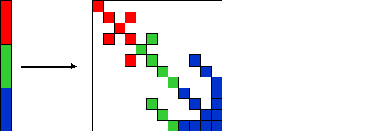
\includegraphics[width=9cm]{sparse-b}

(c)

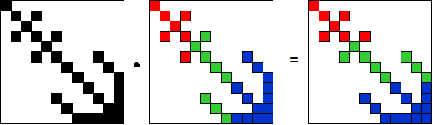
\includegraphics[width=10cm]{sparse-c}

(d)

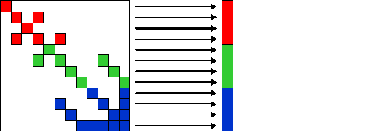
\includegraphics[width=9cm]{sparse-d}

\caption{\label{cap:SparseMatrix}Schematic representation of a numerical sparse
matrix-dense vector multiply.}

\end{figure}


The use of Global Array operations in implementing this operation
is described in more detail below. The original dense vector and final
product vector are assumed to be located in distributed 1D Global
Arrays with handles \texttt{g\_b} and \texttt{g\_c}, respectively.
The first step in performing the multiply operation is to create a
1D Global Array that is the same size as the original compressed matrix
VALUES array and has the same distribution across processors. Denoting
the handle of this array as \texttt{g\_tmp}, it can be filled with
the following sequence of operations
\begin{verbatim}
call~nga\_distribution(g\_j\_index,~me,~lo,~hi)~

call~nga\_access(g\_j\_index,~lo,~hi,~idx,~ld)~

call~nga\_access(g\_tmp,~lo,~hi,~id\_tmp,~ld)~

ld~=~hi~\textendash{}~lo~+~1~

call~nga\_gather(g\_b,~dbl\_mb(id\_tmp),int\_mb(idx),ld)~

call~nga\_release(g\_j\_index,~lo,~hi)~

call~nga\_release(g\_tmp,lo,hi)
\end{verbatim}
The first three lines find the location in memory of the local portions
of the J-VALUES vector and the \texttt{g\_tmp} array. These should
both correspond to the same values of \texttt{lo} and \texttt{hi}.
The \texttt{nga\_gather} operation then copies the values of \texttt{g\_b}
in the locations pointed to by the j values represented by the index
\texttt{idx} into the corresponding locations of the local portion
of \texttt{g\_tmp}. The remaining lines release access to the local
data. Although this operation can be expressed in only a few lines
of code, it is quite complicated in terms of how it manipulates data
and may be worth spending some additional time to understand how it
works.

The element-wise multiplication of the \texttt{g\_tmp} and \texttt{g\_values}
arrays can be trivially implemented with a single call to \texttt{ga\_elem\_multiply}(\texttt{g\_tmp},
\texttt{g\_values},\texttt{ g\_tmp}). Similarly, the sum across rows
in the \texttt{g\_tmp} array can be accomplished by calling \texttt{ga\_scan\_add}(\texttt{g\_tmp},
\texttt{g\_values}, \texttt{g\_mask}, \texttt{one}, \texttt{ntot},
\texttt{0}), where \texttt{ntot} is the total number of non-zero elements.
At this point the values of the product vector are located at the
elements just before the locations indicated by the g\_mask array.
To get these values back into an ordinary compressed vector, the g\_mask
vector is shifted to the left by one place, using the following code
fragment
\begin{verbatim}
call~nga\_distribution~(g\_mask,~me,~lo,~hi)~

call~nga\_access(g\_mask,~lo,~hi,~idx,~ld)~

ld~=~hi-lo~

isav~=~int\_mb(idx)~

do~i~=~1,~ld~

~~~int\_mb(idx~+~i~\textendash{}~1)~=~int\_mb(idx~+~i)~

end~do~

if~(lo.eq.1)~then~

~~~ldx~=~isize~

else~

~~~idx~=~lo-1~

endif~call~

nga\_release(g\_mask,~lo,~hi)~

call~ga\_sync~

call~nga\_put(g\_mask,~idx,~idx,~isav,~ld)~

call~g\_sync
\end{verbatim}
The results in \texttt{g\_tmp} can now be packed into the final results
vector \texttt{g\_c} using a single call to \texttt{ga\_pack}(\texttt{t\_tmp},
\texttt{g\_c}, \texttt{g\_mask}, \texttt{one}, \texttt{ntot}, \texttt{icnt}). 


\chapter{Restricted Arrays}

\include{\string"Section12-Restricted-Arrays\string"}

%\chapter{Appendix A - List of C Functions}

%\href{http://www.emsl.pnl.gov/docs/global/Capi.html}{Online listing of C functions. }

%\chapter{Appendix B - List of Fortran Functions}

%\href{http://www.emsl.pnl.gov/docs/global/GAapi.html}{Online listing of Fortran functions. }

\chapter{Appendix C - Global Arrays on Older Systems}

\label{Appendix_C}Global Arrays supports many computing platforms.
This appendix discusses those platforms, including older systems.

The web page \url{www.emsl.pnl.gov/docs/global/support.html} contains
updated information about using GA on different platforms. Please
refer to this page frequently for most recent updates and platform
information. 


\section{Platform and Library Dependencies }

The following platforms are supported by Global Arrays. 


\section{Supported Platforms}
\begin{itemize}
\item IBM SP, CRAY T3E/J90/SV1, SGI Origin, Fujitsu VX/VPP, Hitachi 
\item Cluster of workstations: Solaris, IRIX, AIX, HPUX, Digital/Tru64 Unix,
Linux, NT 
\item Standalone uni- or multi-processor workstations or servers 
\item Standalone uni- or multi-processor Windows NT workstations or servers
\end{itemize}
Older versions of GA supported some additional (now obsolete) platforms
such as: IPSC, KSR, PARAGON, DELTA, CONVEX. They are not supported
in the newer (>3.1) versions because we do not have access to these
systems. We recommend using GA 2.4 on these platforms.

For most of the platforms, there are two versions available: 32-bit
and 64-bit. This table specifies valid TARGET names for various supported
platforms. 

\begin{longtable}{|>{\centering}p{3cm}|c|>{\centering}p{3cm}|>{\centering}p{3cm}|}
\hline 
Platform & 32-bit TARGET name & 64-bit TARGET name & Remarks\tabularnewline
\hline
\endhead
\hline 
Sun Ultra & SOLARIS & SOLARIS64 & 64-bit version added in GA 3.1\tabularnewline
\hline 
IBM BlueGene/P &  & BGP & supported in GA 4.1 and later (Contact your BlueGene sys admin for
GA instalation). More info in support page...\tabularnewline
\hline 
IBM BlueGene/L &  & BGL & added in GA 4.0.2 (Contact your BlueGene sys admin for GA instalation).
More info in support page...\tabularnewline
\hline 
Cray XT3/XT4 &  & LINUX64 (or) CATAMOUNT & TARGET based on the OS in compute Nodes (Catamount/Linux). More info
and sample settings in support page...\tabularnewline
\hline 
IBM RS/6000 & IBM & IBM64 & 64-bit version added in GA 3.1\tabularnewline
\hline 
IBM SP & LAPI & LAPI64 & no support yet for user-space communication in the 64-bit mode by
IBM\tabularnewline
\hline 
Compaq/DEC alpha & not available & DECOSF & \tabularnewline
\hline 
HP pa-risc & HPUX & HPUX64 & 64-bit version added in GA 3.1\tabularnewline
\hline 
Linux (32-bit): x86, ultra, powerpc & LINUX & not available & \tabularnewline
\hline 
Linux (64-bit): ia64 (Itanium), x86\_64 (Opteron), ppc64, etc & not available & LINUX64 & \tabularnewline
\hline 
Linux alpha & not available & LINUX64 & 64-bit version added in GA 3.1; Compaq compilers rather than GNU required\tabularnewline
\hline 
Cray T3E & not available & CRAY-T3E & \tabularnewline
\hline 
Cray J90 & not available & CRAY-YMP & \tabularnewline
\hline 
Cray SV1 & not available & CRAY-SV1 & \tabularnewline
\hline 
Cray X1 & not available & CRAY-SV2 & In X1, by default, TARGET is defined by the operating system as cray-sv2\tabularnewline
\hline 
SGI IRIX mips & SGI\_N32, SGI & SGIFP & \tabularnewline
\hline 
Hitachi SR8000 & HITACHI & not available & \tabularnewline
\hline 
Fujitsu VPP systems & FUJITSU-VPP & FUJITSU-VPP64 & 64-bit version added in GA 3.\tabularnewline
\hline 
NEC SX series &  & NEC & \tabularnewline
\hline 
Apple & MACX & MACX64 & Running MAC X or higher\tabularnewline
\hline
\end{longtable}

To aid development of fully portable applications, in 64-bit mode
Fortran integer datatype is 64-bits. It is motivated by 1) the need
of applications to use very large data structures and 2) Fortran INTEGER{*}8
not being fully portable. The 64-bit representation of integer datatype
is accomplished by using the appropriate Fortran compiler flag.

Because of limited interest in heterogenous computing among known
GA users, the Global Arrays library \emph{still does not support heterogeonous
platforms}. This capability can be added if required by new applications. 


\section{Selection of the communication network for ARMCI }

Some cluster installations can be equipped with a high performance
network which offer instead, or in addition to TCP/IP some special
communication protocol, for example GM on Myrinet network. To achieve
high performance in Global Arrays, \href{http://www.emsl.pnl.gov/docs/parsoft/armci}{ARMCI}
must be built to use these protocols in its implementation of one-sided
communication. Starting with GA 3.1, this is accomplished by setting
an environment variable ARMCI\_NETWORK to specify the protocol to
be used. In addition, the it might be necessary to provide location
for the header files and library path corresponding to location of
s/w supporting the appropriate protocol API, see g/armci/config/makecoms.h
for details. 

\begin{tabular}{|c|c|>{\centering}p{3cm}|>{\centering}p{3cm}|}
\hline 
Network & Protocol Name & ARMCI\_NETWORK Setting & Supported Platforms\tabularnewline
\hline
\hline 
Ethernet & TCP/IP & SOCKETS (optional/default) & workstation clusters (32 and 64-bit)\tabularnewline
\hline 
Quadrics/QsNet & Elan3/Shmem & QUADRICS or ELAN3 & Linux (alpha,x86,IA64,..), Compaq \tabularnewline
\hline 
Quadrics/QsNet II & Elan4 & ELAN4 & Linux (32 and 64-bit) \tabularnewline
\hline 
Infiniband & OpenIB & OPENIB & Linux (32 and 64-bit). NOTE: This network is supported in GA versions>=4.1.
For more info see the \href{http://www.emsl.pnl.gov/docs/global/support.html}{Support}
page...\tabularnewline
\hline 
Infiniband & VAPI & MELLANOX & Linux (32 and 64-bit)\tabularnewline
\hline 
Myrinet & GM & GM & Linux (x86,ultra,IA64)\tabularnewline
\hline 
Giganet cLAN & VIA & VIA & Linux (32 and 64-bit)\tabularnewline
\hline 
 & MPI & MPI-SPAWN & Supported in GA 4.1 or higher. This network setting can be used on
any platform that has MPI-2 dynamic process management support. Using
this setting is recommended only if your network is not listed above.\tabularnewline
\hline
\end{tabular}

\emph{Other Platforms:} (More settings info for these platforms in
the\href{http://www.emsl.pnl.gov/docs/global/support.html}{Support}
page) 

\begin{tabular}{|c|c|c|}
\hline 
Platforms & Protocol Name & ARMCI\_NETWORK Setting\tabularnewline
\hline
\hline 
IBM BG/L & BGML & BGMLMPI \tabularnewline
\hline 
Cray XT3/XT4  & Shmem Portals  & CRAY-SHMEM PORTALS 2.1.3\tabularnewline
\hline
\end{tabular}


\section{Selection of the message-passing library }

As explained in Section \ref{sec:Initialization-and-Termination},
GA works with either MPI or TCGMSG message-passing libraries. That
means that GA applications can use either of these interfaces. Selection
of the message-passing library takes place when GA is built. Since
the TCGMSG library is small and compiles fast, it is included with
the GA distribution package and built on Unix workstations by default
so that the package can be built as fast and as convenientlly to the
user as possible. There are three possible configurations for running
GA with the message-passing libraries:
\begin{enumerate}
\item \textcolor{black}{\underbar{GA with MPI}} (\emph{recommended}): directly
with MPI. In this mode, GA program should contain MPI initialization
calls. 
\item \textcolor{black}{\underbar{GA with TCGMSG-MPI}} (MPI and TCGMSG emulation
library): TCGMSG-MPI implements functionality of TCGMSG using MPI.
In this mode, the message passing library is initialized using a TCGMSG
PBEGIN(F) call which internally references MPI\_Initialize. To enable
this mode, define the environmental variable USE\_MPI. 
\item \textcolor{black}{\underbar{GA with TCGMSG}}: directly with TCGMSG.
In this mode, GA program should contain TCGMSG initialization calls.
\end{enumerate}
For the MPI versions, the optional environmental variables MPI\_LIB
and MPI\_INCLUDE are used to point to the location of the MPI library
and include directories if they are not in the standard system location(s).
GA programs are started with the mechanism that any other MPI programs
use on the given platform.

The recent versions of MPICH (an MPI implementation from ANL/Mississippi
State) keep the MPI header files in more than one directory and provide
compiler wrappers that implicitly point to the appropriate header
files. One can :
\begin{itemize}
\item use MPI\_INCLUDE by expanding the string with another directory component
prefixed with \textquotedbl{}-I\textquotedbl{} (you are passing include
directory names as a part of compiler flags), or (starting with GA
3.1) separated by comma \textquotedbl{},\textquotedbl{} and withot
the prefix, OR 
\item use MPI aware compiler wrappers e.g., mpicc and mpif77 to build GA
right out of the box on UNIX workstations: \end{itemize}
\begin{lyxcode}
make~FC=mpif77~CC=mpicc~
\end{lyxcode}
One disadvantage of the second approach it that GA makefile in some
circumstances might be not able to determine which compiler (e.g.,
GNU or PGI) is called underneath by the MPICH compiler wrappers. Since
different compilers provide different Fortran/C interface, the package
might fail to build. This problem is most likely to occur on non-Linux
Unix systems with non-native compilers (e.g., gcc).

On Windows NT, the current version of GA was tested with WMPI, an
NT implementation derived from MPICH in Portugal. 


\section{Dependencies on other software }

In addition to the message-passing library, GA requires:
\begin{itemize}
\item \href{http://www.emsl.pnl.gov/docs/parsoft/ma/MAapi.html}{MA}MA (Memory
Allocator), a library for managment of local memory; 
\item \href{http://www.emsl.pnl.gov/docs/parsoft/armci}{ARMCI}, a one-sided
communication library that GA uses as its run-time system; 
\item BLAS library is required for the eigensolver and ga\_dgemm; 
\item LAPACK library is required for the eigensolver (a subset is included
with GA, which is built into \emph{liblinalg.a});
\end{itemize}
GA may also depend on other software depending on the functions being
used.
\begin{itemize}
\item GA eigensolver, ga\_diag, is a wrapper for the eigensolver from the
PEIGS library; (Please contact \href{mailto:fanngi@ornl.gov}{George Fann}about
PEIGS) 
\item SCALAPACK, PBBLAS, and BLACS libraries are required for \emph{ga\_lu\_solve,
ga\_cholesky, ga\_llt\_solve, ga\_spd\_invert, ga\_solve}. If these
libraries are not installed, the named operations will not be available. 
\item If one would like to generate trace information for GA calls, an additional
library \emph{libtrace.a} is required, and the -DGA\_TRACE define
flag should be specified for C and Fortran compilers.
\end{itemize}

\section{Writing GA Programs }

C programs that use Global Arrays should include files \emph{`global.h',
'ga.h', `macdecls.h'}. Fortran programs should include the files \emph{`mafdecls.fh',
`global.fh'}. Fortran source must be preprocessed as a part of compilation.

The GA program should look like:
\begin{itemize}
\item When GA runs with MPI\end{itemize}
\begin{lyxcode}
\textcolor{blue}{Fortran~}~~~~~~~~~~~~~~\textcolor{green}{C}

\textcolor{blue}{call~mpi\_init(..)~}~~~\textcolor{green}{MPI\_Init(..)~}~~~!~start~MPI~

\textcolor{blue}{call~ga\_initialize()}~\textcolor{green}{GA\_Initialize()~}!~start~global~arrays~

\textcolor{blue}{status~=~ma\_init(..)}~\textcolor{green}{MA\_Init(..)~}~~~~!~start~memory~allocator

\textcolor{blue}{....~do~work~~}~~~~~~~\textcolor{green}{....~do~work}

\textcolor{blue}{call~ga\_terminate()}~~\textcolor{green}{GA\_Terminate()~}~!~tidy~up~global~arrays~call

\textcolor{blue}{mpi\_finalize()}~~~~~~~\textcolor{green}{MPI\_Finalize()}~~!~tidy~up~MPI~~

\textcolor{blue}{stop}~~~~~~~~~~~~~~~~~~~~~~~~~~~~~~~~~!~exit~program\end{lyxcode}
\begin{itemize}
\item When GA runs with TCGMSG or TCGMSG-MPI\end{itemize}
\begin{lyxcode}
\textcolor{blue}{Fortran~C}

\textcolor{blue}{call~pbeginf()~}~~~~~~~~\textcolor{green}{PBEGIN\_(..)~}~~~~!~start~TCGMSG~

\textcolor{blue}{call~ga\_initialize()}~~~\textcolor{green}{GA\_Initialize()}~!~start~global~arrays~

\textcolor{blue}{status~=~ma\_init(..)}~~~\textcolor{green}{MA\_Init(..)}~~~~~!~start~memory~allocator

\textcolor{blue}{....~do~work~}~~~~~~~~~~~\textcolor{green}{....~do~work}

\textcolor{blue}{call~ga\_terminate()}~~~~\textcolor{green}{GA\_Terminate()~}~!~tidy~up~global~arrays~

\textcolor{blue}{call~pend()}~~~~~~~~~~~~\textcolor{green}{PEND\_()}~~~~~~~~~!~tidy~up~tcgmsg~

\textcolor{blue}{stop~}~~~~~~~~~~~~~~~~~~~~~~~~~~~~~~~~~~!~exit~program~
\end{lyxcode}
The \emph{ma\_init }call looks like :
\begin{lyxcode}
status~=~ma\_init(type,~stack\_size,~heap\_size)
\end{lyxcode}
and it basically just goes to the OS and gets \emph{stack\_size+heap\_size}
elements of size type. The amount of memory MA allocates need to be
sufficient for storing global arrays on some platforms. Please refer
to section \ref{sub:Memory-Allocation} for the details and information
on more advanced usage of MA in GA programs. 


\section{Building GA }

Use\emph{ GNU make} to build the GA library and application programs
on Unix and Microsoft nmake on Windows. The structure of the available
makefiles are
\begin{itemize}
\item GNUmakefile: Unix makefile 
\item MakeFile: Windows NT makefile 
\item config/makefile.h: definitions \& include symbols
\end{itemize}
The user must specify TARGET as an environment variable (setenv TARGET
TARGET\_name) or in the GNUmakefile or on the command line when calling
make. For example: 

(for IBM/SP platform)
\begin{lyxcode}
setenv~TARGET~LAPI~
\end{lyxcode}
(or) from the command line, 
\begin{lyxcode}
gmake~TARGET=LAPI
\end{lyxcode}
Valid TARGET\_name for various supported platforms can be found in
the above table. Valid TARGETs can also be listed by calling make
in the top level distribution directory on UNIX family of systems
when TARGET is not defined. On Windows, WIN32, CYGNUS and INTERIX
(previously known as OpenNT) are supported. 


\paragraph{Compiler Settings (optional): }

For various supported platforms, the default compilers and compiler
options are specified in config/makefile.h. One could change the predefined
default compilers and compiler flags in GA package either by specifying
them on the command line or in the file config/makefile.h. Note: editing
config/makefile.h for any platform requires extra care and is intended
for intermediate/advanced users.
\begin{itemize}
\item CC - name of the C compiler (e.g., gcc, cc, or ccc ) 
\item FC - name of the Fortran compiler (e.g., g77, f90, mpif77 or fort) 
\item COPT - optimization or debug flags for the C compiler (e.g., -g, -O3) 
\item FOPT - optimization or debug flags for the Fortran compiler (e.g.,
-g, -O1)
\end{itemize}
For example,
\begin{lyxcode}
gmake~FC=f90~CC=cc~FOPT=-O4~COPT=-g
\end{lyxcode}
Note that GA provides only Fortran-77 interfaces. To use and compile
with a Fortran 90 compiler, it has to support a subset of Fortran-77. 


\subsection{Unix Environment }

As mentioned in an earlier section, there are three possible configurations
for building GA.
\begin{enumerate}
\item \textcolor{black}{\underbar{GA with MPI}} (recommended): To build
GA directly with MPI, the user needs to define environmental variables
MPI\_LIB and MPI\_INCLUDE which should point to the location of the
MPI library and include directories. Additionally, the make/environmental
variable MSG\_COMMS must be defined as MSG\_COMMS = MPI. (In csh/tcsh,
setenv MSG\_COMMS MPI)
\item \textcolor{black}{\underbar{GA with TCGMSG-MPI}}: To build GA with
the TCGMSG-MPI, user needs to define environmental variables USE\_MPI,
MPI\_LIB and MPI\_INCLUDE which should point to the location of the
MPI library and include directories.


\emph{Example}: using csh/tcsh (assume using MPICH installed in /usr/local
on IBM workstation)
\begin{lyxcode}
setenv~USE\_MPI~y~

setenv~MPI\_LOC~/usr/local/mpich~

setenv~MPI\_LIB~\$MPI\_LOC/lib/rs6000/ch\_shmem~

setenv~MPI\_INCLUDE~\$MPI\_LOC/include
\end{lyxcode}
\item \textcolor{black}{\underbar{GA with TCGMSG}}: To build GA directly
with TCGMSG, the user must define the environmental variable MSG\_COMMS=TCGMSG.
Note: When MSG\_COMMS=TCGMSG, make sure to unset the environment variable
USE\_MPI (e.g. unsetenv USE\_MPI).
\end{enumerate}
After chosing the configuration, to build the GA library, type 
\begin{lyxcode}
make~
\end{lyxcode}
or 
\begin{lyxcode}
gmake
\end{lyxcode}
If the build is successful, a test program test.x will be created
in global/testing directory. Refer to the Section \textquotedbl{}Running
GA programs\textquotedbl{} on how to run this test.

To build an application based on GA located in g/global/testing, for
example, the application's name is app.c (or app.F, app.f), type 
\begin{lyxcode}
make~app.x~
\end{lyxcode}
or 
\begin{lyxcode}
gmake~app.x
\end{lyxcode}
Please refer to compiler flags in file g/config/makefile.h to make
sure that Fortran and C compiler flags are consistent with flags uses
to compile your application. This may be critical when Fortran compiler
flags are used to change the default length of the integer datatype.


\paragraph{Interface to ScaLAPACK}

GA interface routines to ScaLAPACK are only available, when GA is
build with MPI and ScaLAPACK. Before building GA, the user is required
to define the environment variables USE\_SCALAPACK or USE\_SCALAPACK\_I8
(for scalapack libraries compiled with 8-byte integers), and the location
of ScaLAPACK \& Co. libraries in the env variable SCALAPACK.

\emph{Example}: using csh/tcsh
\begin{lyxcode}
setenv~USE\_SCALAPACK~y~(or)~setenv~USE\_SCALAPACK\_I8~y~

setenv~SCALAPACK~'-L/msrc/proj/scalapack/LIB/rs6000~

~~~~~~~-lscalapack~-lpblas~-ltools~-lblacsF77cinit~-lblacs'~

setenv~USE\_MPI~y
\end{lyxcode}
Since there are certain interdependencies between blacs and blacsF77cinit,
some system might require specification of -lblacs twice to fix the
unresolved external symbols from these libs.


\paragraph{Installing GA C++ Bindings}

By default, GA C++ bindings are not built. GA++ is built only if GA\_C\_CORE
is defined as follows: 
\begin{lyxcode}
setenv~GA\_C\_CORE~y~

cd~GA\_HOME~

make~clean;~make~
\end{lyxcode}
(This will build GA with C core and C++ binding).


\paragraph{Using GA\_C\_CORE}

GA's internal core is implemented using Fortran and C. When GA\_C\_CORE
is set, core Fortran functionalites are replaced by their C counterparts
to eliminate the hassle involved in mixing Fortran and C with C++
bindings on certain platforms or for some compilers (like, missing
Fortran symols/libraries during the linking phase). NOTE: C and C++
compilers should be from the same family. GA\_C\_CORE doesnot support
mixing C and C++ compilers (e.g.using Intel compiler for C and GNU
compiler for C++). 
\begin{lyxcode}
make~FC=ifort~CC=icc~CXX=g++~(not~supported~if~GA\_C\_CORE~is~set)~

make~FC=ifort~CC=icc~CXX=icpc~(Intel~compiler~family~-~supported)
\end{lyxcode}

\subsection{Windows NT }

To buid GA on Windows NT, MS Power Fortran 4 or DEC Visual Fortran
5 or later, and MS Visual C 4 or later are needed. Other compilers
might need the default compilation flags modified. When commercial
Windows compilers are not available, one can choose to use CYGNUS
or INTERIX and build it as any other Unix box using GNU compilers.

First of all, one needs to set environment variables (same as in Unix
enviroment). GA needs to know where find the MPI include files and
libraries. To do this, select the Environment tab under the Control
Panel, then set the variables to point to the location of MPI, for
example for WMPI on disk D:
\begin{lyxcode}
set~MPI\_INCLUDE~as~d:\textbackslash{}Wmpi\textbackslash{}Include~

set~MPI\_LIB~as~d:\textbackslash{}Wmpi\textbackslash{}Console
\end{lyxcode}
Make sure that the dynamic link libraries required by the particular
implementation of MPI are copied to the appropriate location for the
system DLLs. For WMPI, copy VWMPI.dll to \textbackslash{}winnt.

In the top directory do,
\begin{lyxcode}
nmake
\end{lyxcode}
The GA test.exe program can be built in the g\textbackslash{}global\textbackslash{}testing
directory:
\begin{lyxcode}
nmake~test.exe
\end{lyxcode}
In addition, the HPVM package from UCSD offers the GA interface in
the NT/Myrinet cluster environment.

GA could be built on Windows 95/98. However, due to the DOS shell
limitations, the top level NTmakefile will not work. Therefore, each
library has to be made separately in its own directory. The environment
variables referring to MPI can be hardcoded in the NT makefiles.


\subsection{Writing and building new GA programs}

For small programs contained in a single file, the most convenient
approach is to put your program file into the g/global/testing directory.
\emph{The existing GNU make suffix rules would build an executable
with the \textquotedbl{}.x\textquotedbl{} suffix from any C or Fortran
source file}. You do not have to modify makefiles in g/global/testing
at all. For example, if your program is contained in myfile.c or myfile.F
and you place it in that directory, all you need to do to create an
executable called myfile.x is to type: 
\begin{lyxcode}
make~myfile.x
\end{lyxcode}
Windows nmake is not as powerful as GNU make - you would need to modify
the NT makefile.

This approach obviously is not feasible for large packages that contain
multiple source files and directories. In that case you need to provide
apropriate definitions in your makefile:
\begin{itemize}
\item to header files located in the include directory, g/include, where
all public header files are copied in the process of building GA 
\item add references to libglobal.a (Unix) global.lib (Windows) and libma.a
(Unix) ma.lib (Windows) in g/lib/\$(TARGET) and for the message-passing
libraries 
\item follow compilation flags for the GA test programs in GNU and Windows
makefiles g/config/makefile.h. The recommended approach is to include
g/config/makefile.h in your makefile.
\end{itemize}
Starting with GA 3.1, one could simplify linking of applications by
including g/armci/config/makecoms.h and g/armci/config/makemp.h that
define all the necessary platform specific libraries that are required
by GA. 2.4 


\section{Running GA Programs }

Assume the GA program app.x had already been built. To run it,

\textbf{\textcolor{black}{Running on shared memory systems and clusters}}\emph{:
}(i.e., network of workstations/linux clusters)

If the app.x is built based on MPI, run the program the same way as
any other MPI programs. 

\emph{Example}: to run on four processes on clusters, use 
\begin{lyxcode}
mpirun~-np~4~app.x
\end{lyxcode}
\emph{Example}: If you are using MPICH (or MPICH-like Implementations),
and mpirun requires a machinefile or hostfile, then run the GA program
same as any other MPI programs. \textit{\textcolor{black}{The only
change required is to make sure the hostnames are specified in a consecutive
manner in the machinefile}}. Not doing this will prevent SMP optimizations
and would lead to poor resource utilization.
\begin{lyxcode}
mpirun~-np~4~-machinefile~machines.txt~app.x
\end{lyxcode}
\emph{Contents of machines.txt}: (Let us say we have two 2-way SMP
nodes (host1 and host2, and correct formats for a 4-processor machinefile
is shown in the table below).

\begin{tabular}{|>{\centering}p{2cm}|>{\centering}p{2cm}|>{\raggedright}p{3cm}|}
\hline 
Correct & Correct & Incorrect\tabularnewline
\hline
\hline 
host1

host1

host2

host2 & host2

host2

host1

host1 & host1

host2

host1 (This is wrong, the same hosts should be specified together)

host2\tabularnewline
\hline
\end{tabular}

If app.x is built based on TCGMSG (not including, Fujitsu, Cray J90,
and Windows, because there are no native ports of TCGMSG), to execute
the program on Unix workstations/servers, one should use the 'parallel'
program (built in tcgmsg/ipcv4.0). After building the application,
a file called 'app.x.p' would also be generated (If there is not such
a file, make it: 
\begin{lyxcode}
make~app.x.p
\end{lyxcode}
This file can be edited to specify how many processors and tasks to
use, and how to load the executables. Make sure that 'parallel' is
accessible (you might copy it into your 'bin' directory). To execute,
type:
\begin{lyxcode}
parallel~app.x~\end{lyxcode}
\begin{enumerate}
\item On MPPs, such as Cray XT3/XT4, or IMB SPs, use the appropriate system
command to specify the number of processors, load and run the programs.
Example: 

\begin{itemize}
\item to run on IBM SP, run as any other parallel programs (i.e., using
\emph{poe}) 
\item to run on Cray XT3/XT4, use \emph{yod}.
\end{itemize}
\item On Microsoft NT, there is no support for TCGMSG, which means you can
only build your application based on MPI. Run the application program
the same way as any other MPI programs. For, WMPI you need to create
the .pg file. Example: \end{enumerate}
\begin{lyxcode}
R:\textbackslash{}nt\textbackslash{}g\textbackslash{}global\textbackslash{}testing>~start~/b~test.exe
\end{lyxcode}

\section{Building Intel Trace Analyzer (VAMPIR) Instrumented Global Arrays}


\subsection{Introduction}

The following topics are covered in this section.
\begin{itemize}
\item New functions needed for the instrumentation 
\item Build instructions 
\item Further information 
\item Known problems
\end{itemize}

\subsection{New Functions Needed for the Instrumentation}
\begin{itemize}
\item To instrument the GA three C-functions are defined (see g/ga\_vt.c): 
\item vampir\_symdef is defined to associate integer identifiers with user
defined states and activities. It handles any errors that might occur. 
\item vampir\_begin is defined to register entering a user defined state.
It uses a global counter called <vampirtrace\_level> to avoid tracing
the use of libraries within libraries. 
\item vampir\_end is defined to register leaving a user defined state.
\end{itemize}
The interfaces of these functions are defined below.
\begin{lyxcode}
void~\textcolor{blue}{vampir\_symdef}~(int~id,~char~{*}state,~char~{*}activity,~

~~~~~~~~~~~~~~~~~~~~char~{*}file,~int~line);~

void~\textcolor{blue}{vampir\_begin}~(int~id,~char~{*}file,~int~line);~

void~\textcolor{blue}{vampir\_end}~(int~id,~char~{*}file,~int~line);
\end{lyxcode}
In addition to these functions two functions are defined to initialise
and finalise MPI when needed. The use of MPI is required because Vampirtrace
uses it internally. The functions are
\begin{lyxcode}
void~\textcolor{blue}{vampir\_init}~(int~argc,~char~{*}{*}argv,~char~{*}file,~

~~~~~~~~~~~~~~~~~~int~line);~

void~\textcolor{blue}{vampir\_finalize}~(char~{*}file,~int~line);
\end{lyxcode}
If the cpp flag -DMPI is provided then these two functions will turn
into null functions. In that case the use of MPI within the GAs will
ensure that Vampirtrace will be initialised properly.

The values for <file> and <line> are substitute with \_\_FILE\_\_
and \_\_LINE\_\_ macros. On compilation the C-preprocessor replaces
these macros with the actual file name and line number. These values
are used to generate error messages if needed. These functions are
defined in the file g/ga\_vt.h.

For each of the instrumented libraries an initialisation routine must
be defined that sets the state and activity tables up.
\begin{itemize}
\item \emph{tcgmsg}: tcgmsg\_vampir\_init in g/tcgmsg/tcgmsg\_vampir.c.
This routine is called from within PBEGINF. 
\item \emph{tcgmsg-mpi}: tcgmsg\_vampir\_init in g/tcgmsg-mpi/tcgmsg\_vampir.c
called from ALT\_PBEGIN\_ in misc.c. 
\item \emph{armci}: armci\_vampir\_init in g/armci/src/armci\_vampir.c called
from ARMCI\_Init in armci.c. 
\item \emph{global}: ga\_vampir\_init in g/global/src/ga\_vampir.c called
from ga\_initialize\_ and ga\_initialize\_ltd\_ in global.armci.c
\end{itemize}

\subsection{Build Instructions }

To build GA with Vampir (now called, Intel Trace Analyzer) set the
environment variable GA\_USE\_VAMPIR.

e.g., \texttt{\textcolor{black}{setenv GA\_USE\_VAMPIR y}}

to compile the GAs including all the Vampirtrace instrumentation.
Further environment variables that are required are
\begin{lyxcode}
LIBVT~:~The~name~of~the~library,~normally~-lVT~which~

~~~~~~~~~~~~~is~the~default.~

VT\_LIB~:~The~path~to~the~library,~-L<library-path>~

~~~~~~~~~~~~~e.g.~setenv~VT\_LIB~/usr/local/vampir/lib~

VT\_INCLUDE:~The~path~to~the~include~file~VT.h,~

~~~~~~~~~~~~-I<include-path>.~e.g.~setenv~VT\_INCLUDE

~~~~~~~~~~~~/usr/local/vampir/include
\end{lyxcode}
On some platforms it may be necessary to set LIBMPI to -lpmpi to load
the MPI profile interfaces that vampirtrace needs.

There are no defaults for VT\_PATH and VT\_INCLUDE. Beyond this point
simply follow the GA make instructions.

\noun{Note: }that libVT.a should be loaded before mpi or pmpi otherwise
the vampirtracing will be ignored. 


\subsection{Further Information }

More information on using Intel Trace Analyzer can be found on the
Intel website at

\href{http://www.intel.com/software/products/cluster/tanalyzer/}{http://www.intel.com/software/products/cluster/tanalyzer/}

From this location Vampir and Vampirtrace can be downloaded for various
platforms including validation licenses if needed.


\subsection{Known Problems}
\begin{itemize}
\item Vampirtrace and LAM-MPI clash
\end{itemize}
In an attempt to produce traces while running with LAM-MPI the program
would always abort in MPI\_Init due to a segmentation violation. The
Pallas website does not mention LAM-MPI at all, but does explicitly
state that Vampirtrace does work with MPICH. Indeed the latter has
been confirmed in tests. Therefore it is not recommended to use the
Vampirtrace instrumentation with LAM-MPI. 

\end{document}
